% Template:     Informe/Reporte LaTeX
% Documento:    Archivo principal
% Versión:      6.8.2 (11/04/2020)
% Codificación: UTF-8
%
% Autor: Pablo Pizarro R.
%        Facultad de Ciencias Físicas y Matemáticas
%        Universidad de Chile
%        pablo@ppizarror.com
%
% Manual template: [https://latex.ppizarror.com/informe]
% Licencia MIT:    [https://opensource.org/licenses/MIT]

% CREACIÓN DEL DOCUMENTO
\documentclass[letterpaper,11pt]{article} % Articulo tamaño carta, 11pt

% INFORMACIÓN DEL DOCUMENTO
\def\titulodelinforme {Laboratorio 1}
\def\temaatratar {Leyes de Ohm y de Kirchhoff}

\def\autordeldocumento {Nombre del autor}
\def\nombredelcurso {Métodos Experimentales}
\def\codigodelcurso {FI2003}

\def\nombreuniversidad {Universidad de Chile}
\def\nombrefacultad {Facultad de Ciencias Físicas y Matemáticas}
\def\departamentouniversidad {Departamento de Física\\FI2003-10 Métodos Experimentales}
\def\imagendepartamento {departamentos/dfi}
\def\imagendepartamentoescala {0.2}
\def\localizacionuniversidad {Santiago, Chile}

% INTEGRANTES, PROFESORES Y FECHAS
\def\tablaintegrantes {
\begin{tabular}{ll}
	Integrantes:
	& \begin{tabular}[t]{l}
		Matías Méndez Zenteno  \\
		Juanpablo Ignacio Pinto Pérez
	\end{tabular} \\
	Profesor:
	& \begin{tabular}[t]{l}
		Sergio Godoy M.
	\end{tabular} \\
	Auxiliar:
	& \begin{tabular}[t]{l}
		Santiago Oñate Robles \\
		Vicente Sepulveda F.\\
		Paloma Vildoso P.
	\end{tabular} \\

	\multicolumn{2}{l}{} \\
	& \\
	\multicolumn{2}{l}{Fecha de realización: \today} \\
	\multicolumn{2}{l}{Fecha de entrega: \today} \\
	\multicolumn{2}{l}{\localizacionuniversidad}
\end{tabular}}{
}

% CONFIGURACIONES
% Template:     Informe/Reporte LaTeX
% Documento:    Configuraciones del template
% Versión:      6.8.2 (11/04/2020)
% Codificación: UTF-8
%
% Autor: Pablo Pizarro R.
%        Facultad de Ciencias Físicas y Matemáticas
%        Universidad de Chile
%        pablo@ppizarror.com
%
% Manual template: [https://latex.ppizarror.com/informe]
% Licencia MIT:    [https://opensource.org/licenses/MIT]

% CONFIGURACIONES GENERALES
\def\addemptypagetwosides {false}  % Añade pag en blanco al imprimir a 2 caras
\def\compilertype {pdf2latex}      % Compilador {pdf2latex,xelatex,lualatex}
\def\defaultinterline {1.0}        % Interlineado por defecto [pt]
\def\defaultnewlinesize {11}       % Tamaño del salto de línea [pt]
\def\documentlang {es-CL}          % Define el idioma del documento
\def\fontdocument {lmodern}        % Tipografía base, ver soportadas en manual
\def\fonttypewriter {tmodern}      % Tipografía de \texttt, ver manual online
\def\fonturl {tt}                  % Tipo de fuente url {tt,sf,rm,same}
\def\importtikz {false}            % Utilizar la librería tikz
\def\pointdecimal {true}           % N° decimales con punto en vez de coma
\def\predocpageromannumber {true}  % Pág. con número romano previo a inicio doc.
\def\predocpageromanupper {false}  % Páginas en número romano en mayúsculas
\def\predocresetpagenumber {true}  % Resetea número de la pag. tras el índice
\def\showlinenumbers {false}       % Muestra los números de línea del documento
\def\usespanishbabel {true}        % Español, desactivar para otros idiomas

% ESTILO PORTADA Y HEADER-FOOTER
\def\disablehfrightmark {false}    % Desactiva el rightmark del header-footer
\def\hfstyle {style1}              % Estilo header-footer (16 estilos)
\def\hfwidthcourse {0.35}          % Tamaño máximo del curso en header-footer
\def\hfwidthtitle {0.6}            % Tamaño máximo del título en header-footer
\def\hfwidthwrap {false}           % Activa el tamaño máximo en header-footer
\def\portraitstyle {style1}        % Estilo portada (20 estilos)

% CONFIGURACIÓN DE LAS LEYENDAS - CAPTION
\def\captionalignment {justified}  % Posición {centered,justified,left,right}
\def\captionlabelformat {simple}   % Formato leyenda {empty,simple,parens}
\def\captionlabelsep {colon}       % Sep. {none,colon,period,space,quad,newline}
\def\captionlessmarginimage {0.1}  % Margen sup/inf de fig. si no hay ley. [cm]
\def\captionlrmargin {2.0}         % Márgenes izq/der de la leyenda [cm]
\def\captionmarginmultimg {0.0}    % Margen izq/der leyendas múltiple img [cm]
\def\captionnumcode {arabic}       % N° código {arabic,alph,Alph,roman,Roman}
\def\captionnumequation {arabic}   % N° ecuaciones {arabic,alph,Alph,roman,Roman}
\def\captionnumfigure {arabic}     % N° figuras {arabic,alph,Alph,roman,Roman}
\def\captionnumsubfigure {alph}    % N° subfiguras {arabic,alph,Alph,roman,Roman}
\def\captionnumsubtable {alph}     % N° subtabla {arabic,alph,Alph,roman,Roman}
\def\captionnumtable {arabic}      % N° tabla {arabic,alph,Alph,roman,Roman}
\def\captiontbmarginfigure {9.35}  % Margen sup/inf de la leyenda en fig. [pt]
\def\captiontbmargintable {7.0}    % Margen sup/inf de la leyenda en tab. [pt]
\def\captiontextbold {false}       % Etiqueta (código,figura,tabla) en negrita
\def\captiontextsubnumbold {false} % N° subfigura/subtabla en negrita
\def\codecaptiontop {true}         % Leyenda arriba del código fuente
\def\figurecaptiontop {false}      % Leyenda arriba de las imágenes
\def\sectioncaptiondelimiter {.}   % Carácter delimitador n° objeto y sección
\def\showsectioncaptioncode {none} % N° sec. código {none,chap,(s/ss/sss/ssss)ec}
\def\showsectioncaptioneqn {none}  % N° sec. ecuación {none,chap,(s/ss/sss/ssss)ec}
\def\showsectioncaptionfig {none}  % N° sec. figuras {none,chap,(s/ss/sss/ssss)ec}
\def\showsectioncaptionmat {none}  % N° matemático {none,chap,(s/ss/sss/ssss)ec}
\def\showsectioncaptiontab {none}  % N° sec. tablas {none,chap,(s/ss/sss/ssss)ec}
\def\subcaptionlabelformat{parens} % Formato leyenda sub. {empty,simple,parens}
\def\subcaptionlabelsep {space}    % Sep. {none,colon,period,space,quad,newline}
\def\tablecaptiontop {true}        % Leyenda arriba de las tablas

% CONFIGURACIÓN DEL ÍNDICE
\def\addindextobookmarks {true}    % Añade el índice a los marcadores del pdf
\def\charafterobjectindex {.}      % Carácter después de n° figura,tabla,código
\def\charnumpageindex {.}          % Carácter número de página en índice
\def\indexdepth {4}                % Profundidad máxima del índice
\def\indexnewpagec {false}         % Nueva página en índice códigos fuente
\def\indexnewpagee {false}         % Nueva página en índice ecuaciones
\def\indexnewpagef {false}         % Nueva página en índice figuras
\def\indexnewpaget {false}         % Nueva página en índice tablas
\def\indexstyle {tfce}             % Estilo {f:figura,t:tabla,c:código,e:ecuación}
\def\indextitlemargin {11.4}       % Margen título índice \insertindextitle [pt]
\def\objectindexindent {false}     % Indenta la lista de objetos
\def\showappendixsecindex {false}  % Título de la sec. de anexos en el índice
\def\showindex {true}              % Muestra el índice
\def\showindexofcontents {true}    % Muestra la lista de contenidos

% ANEXO, CITAS, REFERENCIAS
\def\apaciterefnumber {false}      % Lista de referencias con números
\def\apaciterefnumberfinal {]}     % Caracter final números apacite
\def\apaciterefnumberinit {[}      % Caracter inicial números apacite
\def\apaciterefsep {9}             % Separación entre refs. {apacite} [pt]
\def\apacitestyle {apacite}        % Formato de ref. apacite {apa,ieeetr,etc..}
\def\appendixindepobjnum {true}    % Anexo usa n° objetos independientes
\def\bibtexrefsep {6}              % Separación entre refs. {bibtex} [pt]
\def\bibtexstyle {apa}             % Formato de ref. bibtex {apa,ieeetr,etc...}
\def\natbibnumbers {true}          % Forza el uso de números en la bibliografía
\def\natbibrefsep {6}              % Separación entre referencia {natbib} [pt]
\def\natbibrefstyle {ieeetr}       % Formato de ref. natbib {apa,ieeetr,etc...}
\def\natbibsquare {true}           % Usa [] o () en las numeraciones
\def\sectionappendixlastchar {.}   % Carácter entre n° de sec. anexo y título
\def\sectionrefenv {false}         % Las referencias se consideran como sección
\def\stylecitereferences {bibtex}  % Estilo cita/ref. {apacite,bibtex,natbib}
\def\twocolumnreferences {false}   % Referencias en dos columnas

% CONFIGURACIONES DE OBJETOS
\def\columnhspace {-0.4}           % Margen horizontal entre obj. \createcolumn
\def\columnsepwidth {2.1}          % Separación entre columnas [em]
\def\defaultimagefolder {img/}     % Carpeta raíz de las imágenes
\def\equationleftalign {false}     % Ecuaciones alineadas a la izquierda
\def\equationrestart {none}        % Reinicio n° {none,chap,(s/ss/sss/ssss)ec}
\def\footnotepagetoprule {false}   % Footnote en pag. tienen separador superior
\def\footnoterestart {none}        % N° footnote {none,chap,page,(s/ss/sss/ssss)ec}
\def\imagedefaultplacement {H}     % Posición por defecto de las imágenes
\def\marginalignbottom {-0.30}     % Margen inferior entorno align [cm]
\def\marginaligncaptbottom {0.05}  % Margen inferior entorno align caption[cm]
\def\marginaligncapttop {-0.60}    % Margen superior entorno align caption [cm]
\def\marginalignedbottom {-0.30}   % Margen inferior entorno aligned [cm]
\def\marginalignedcaptbottom {0.0} % Margen inferior entorno aligned caption[cm]
\def\marginalignedcapttop {-0.60}  % Margen superior entorno aligned caption[cm]
\def\marginalignedtop {-0.40}      % Margen superior entorno aligned [cm]
\def\marginaligntop {-0.40}        % Margen superior entorno align [cm]
\def\margineqncaptionbottom {0.0}  % Margen inferior caption ecuación [cm]
\def\margineqncaptiontop {-0.65}   % Margen superior caption ecuación [cm]
\def\margineqnindexbottom {-0.90}  % Margen inferior ecuaciones índice [cm]
\def\margineqnindextop {-0.25}     % Margen superior ecuaciones índice [cm]
\def\marginequationbottom {-0.15}  % Margen inferior ecuaciones [cm]
\def\marginequationtop {0.0}       % Margen superior ecuaciones [cm]
\def\marginfloatimages {-13.0}     % Margen sup. fig. insertimageleft/right [pt]
\def\marginfootnote {10.0}         % Margen derecho footnote [pt]
\def\margingatherbottom {-0.20}    % Margen inferior entorno gather [cm]
\def\margingathercaptbottom {0.05} % Margen inferior entorno gather caption [cm]
\def\margingathercapttop {-0.77}   % Margen superior entorno gather [cm]
\def\margingatheredbottom {-0.10}  % Margen inf. entorno gathered [cm]
\def\margingatheredcaptbottom{0.0} % Margen inf. entorno gathered caption [cm]
\def\margingatheredcapttop {-0.77} % Margen superior entorno gathered [cm]
\def\margingatheredtop {-0.40}     % Margen superior entorno gathered [cm]
\def\margingathertop {-0.40}       % Margen superior entorno gather [cm]
\def\marginimagebottom {-0.15}     % Margen inferior figura [cm]
\def\marginimagemultright {0.50}   % Margen derecho imágenes múltiples [cm]
\def\marginimagemulttop {-0.30}    % Margen superior imágenes múltiples [cm]
\def\marginimagetop {0.0}          % Margen superior figuras [cm]
\def\numberedequation {true}       % Ecuaciones con \insert... numeradas
\def\sourcecodefontf {\ttfamily}   % Tipo de letra código fuente
\def\sourcecodefonts {\small}      % Tamaño letra código fuente
\def\sourcecodenumbersep {6}       % Separación entre número línea y código [pt]
\def\sourcecodetabsize {3}         % Tamaño tabulación código fuente
\def\tabledefaultplacement {H}     % Posición por defecto de las tablas
\def\tablepaddingh {0.85}          % Espaciado horizontal de celda de las tablas
\def\tablepaddingv {1.05}          % Espaciado vertical de celda de las tablas
\def\tikzdefaultplacement {H}      % Posición por defecto de las figuras tikz

% CONFIGURACIÓN DE LOS TÍTULOS
\def\anumsecaddtocounter {false}   % Insertar títulos anum. aumenta n° de sec
\def\fontsizessstitle{\normalsize} % Tamaño sub-sub-subtítulos
\def\fontsizesubsubtitle {\large}  % Tamaño sub-subtítulos
\def\fontsizesubtitle {\Large}     % Tamaño subtítulos
\def\fontsizetitle {\LARGE}        % Tamaño títulos
\def\fontsizetitlei {\LARGE}       % Tamaño títulos en el índice
\def\showdotaftersnum {true}       % Punto al final de n° (s/ss/sss/ssss)ection
\def\stylessstitle {\bfseries}     % Estilo sub-sub-subtítulos
\def\stylesubsubtitle {\bfseries}  % Estilo sub-subtítulos
\def\stylesubtitle {\bfseries}     % Estilo subtítulos
\def\styletitle {\bfseries}        % Estilo títulos
\def\styletitlei {\bfseries}       % Estilo títulos en el índice

% CONFIGURACIÓN DE LOS COLORES DEL DOCUMENTO
\def\captioncolor {black}          % Color nombre objeto (código,figura,tabla)
\def\captiontextcolor {black}      % Color de la leyenda
\def\colorpage {white}             % Color de la página
\def\highlightcolor {yellow}       % Color del subrayado con \hl
\def\indextitlecolor {black}       % Color de los títulos del índice
\def\linenumbercolor {gray}        % Color del n° de línea (\showlinenumbers)
\def\linkcolor {black}             % Color de los links del documento
\def\maintextcolor {black}         % Color principal del texto
\def\numcitecolor {black}          % Color del n° de las referencias o citas
\def\portraittitlecolor {black}    % Color de los títulos de la portada
\def\showborderonlinks {false}     % Color de un link por un recuadro de color
\def\sourcecodebgcolor {lgray}     % Color de fondo del código fuente
\def\ssstitlecolor {black}         % Color de los sub-sub-subtítulos
\def\subsubtitlecolor {black}      % Color de los sub-subtítulos
\def\subtitlecolor {black}         % Color de los subtítulos
\def\tablelinecolor {black}        % Color de las líneas de las tablas
\def\tablerowfirstcolor {none}     % Primer color de celda de las tablas
\def\tablerowsecondcolor {gray!20} % Segundo color de celda de las tablas
\def\titlecolor {black}            % Color de los títulos
\def\urlcolor {magenta}            % Color de los enlaces web (\href,\url)

% MÁRGENES DE PÁGINA
\def\firstpagemargintop {3.8}      % Margen superior página portada [cm]
\def\pagemarginbottom {2.7}        % Margen inferior página [cm]
\def\pagemarginleft {2.54}         % Margen izquierdo página [cm]
\def\pagemarginright {2.54}        % Margen derecho página [cm]
\def\pagemargintop {3.0}           % Margen superior página [cm]

% OPCIONES DEL PDF COMPILADO
\def\cfgbookmarksopenlevel {1}     % Nivel marcadores en pdf (1:secciones)
\def\cfgpdfbookmarkopen {true}     % Expande marcadores del nivel configurado
\def\cfgpdfcenterwindow {true}     % Centra ventana del lector al abrir el pdf
\def\cfgpdfcopyright {}            % Establece el copyright del documento
\def\cfgpdfdisplaydoctitle {true}  % Muestra título del informe en visor
\def\cfgpdffitwindow {false}       % Ajusta la ventana del lector tamaño pdf
\def\cfgpdfkeywords {}             % Palabras clave del pdf
\def\cfgpdfmenubar {true}          % Muestra el menú del lector
\def\cfgpdfpagemode {OneColumn}    % Modo de página {OneColumn,SinglePage}
\def\cfgpdfpageview {FitH}         % {Fit,FitH,FitV,FitR,FitB,FitBH,FitBV}
\def\cfgpdfsecnumbookmarks {true}  % Número de la sec. en marcadores del pdf
\def\cfgpdftoolbar {true}          % Muestra barra de herramientas lector pdf
\def\cfgshowbookmarkmenu {false}   % Muestra menú marcadores al abrir el pdf
\def\pdfcompilecompression {9}     % Factor de compresión del pdf (0-9)
\def\pdfcompileobjcompression {2}  % Nivel compresión objetos del pdf (0-3)
\def\pdfcompileversion {7}         % Versión mínima del pdf compilado

% NOMBRE DE OBJETOS
\def\nameabstract {Resumen}           % Nombre del resumen-abstract
\def\nameappendixsection {Anexos}     % Nombre de los anexos
\def\namemathcol {Corolario}          % Nombre de los colorarios
\def\namemathdefn {Definición}        % Nombre de las definiciones
\def\namemathej {Ejemplo}             % Nombre de los ejemplos
\def\namemathlem {Lema}               % Nombre de los lemas
\def\namemathobs {Observación}        % Nombre de las observaciones
\def\namemathprp {Proposición}        % Nombre de las proposiciones
\def\namemaththeorem {Teorema}        % Nombre de los teoremas
\def\nameportraitpage {Portada}       % Etiqueta página de la portada
\def\namereferences {Referencias}     % Nombre de la sección de referencias
\def\nomchapter {Capítulo}            % Nombre de los capítulos
\def\nomltappendixsection {Anexo}     % Etiqueta sección en anexo/apéndices
\def\nomltcont {Índice de Contenidos} % Nombre del índice de contenidos
\def\nomlteqn {Índice de Ecuaciones}  % Nombre de la lista de ecuaciones
\def\nomltfigure {Índice de Figuras}  % Nombre de la lista de figuras
\def\nomltsrc {Índice de Códigos}     % Nombre de la lista de código
\def\nomlttable {Índice de Tablas}    % Nombre de la lista de tablas
\def\nomltwfigure {Figura}            % Etiqueta leyenda de las figuras
\def\nomltwsrc {Código}               % Etiqueta leyenda del código fuente
\def\nomltwtable {Tabla}              % Etiqueta leyenda de las tablas
\def\nomnpageof { de }                % Etiqueta página # de #


% IMPORTACIÓN DE LIBRERÍAS
% Template:     Informe/Reporte LaTeX
% Documento:    Importación de librerías
% Versión:      6.8.2 (11/04/2020)
% Codificación: UTF-8
%
% Autor: Pablo Pizarro R.
%        Facultad de Ciencias Físicas y Matemáticas
%        Universidad de Chile
%        pablo@ppizarror.com
%
% Manual template: [https://latex.ppizarror.com/informe]
% Licencia MIT:    [https://opensource.org/licenses/MIT]

\let\RE\Re
\let\IM\Im
\let\counterwithout\relax
\let\counterwithin\relax
\let\underbar\relax
\let\underline\relax
\def\unaccentedoperators{}
\def\decimalpoint{}
\def\bibname{}
\makeatletter
\def\underline#1{\relax\ifmmode\@@underline{#1}\else $\@@underline{\hbox{#1}}\m@th$\relax\fi}\def\underbar#1{\underline{\sbox\tw@{#1}\dp\tw@\z@\box\tw@}}
\makeatother
\usepackage{ifthen}
\ifthenelse{\equal{\usespanishbabel}{true}}{
	\usepackage[spanish,es-nosectiondot,es-lcroman,es-noquoting]{babel}}{
}
\usepackage{sectsty}
\ifthenelse{\equal{\compilertype}{pdf2latex}}{
	\usepackage[utf8]{inputenc}}{
}
\newcommand{\throwbadconfig}[4][]{
	\ifthenelse{\equal{#1}{noheader}}{
		\errmessage{LaTeX Warning: #4}
	}{
		\ifthenelse{\equal{#1}{noheader-nostop}}{
			\errmessage{LaTeX Warning: #4}
		}{
			\errmessage{LaTeX Warning: #2 \noexpand #3=#3. Valores esperados: #4}
		}
	}
	\ifthenelse{\equal{#1}{nostop}}{}{
		\ifthenelse{\equal{#1}{noheader-nostop}}{}{
			\stop
		}
	}
}
\ifthenelse{\equal{\equationleftalign}{true}}{
	\usepackage[fleqn]{amsmath}
}{
	\usepackage{amsmath}
}
\usepackage{amssymb}
\usepackage{amsthm}
\usepackage{array}
\usepackage{bigstrut}
\usepackage{bm}
\usepackage{booktabs}
\usepackage{caption}
\usepackage{changepage}
\usepackage{chngcntr}
\usepackage{color}
\usepackage{datetime}
\usepackage{floatpag}
\usepackage{floatrow}
\usepackage{framed}
\usepackage{gensymb}
\usepackage{graphicx}
\usepackage{lipsum}
\usepackage{listings}
\usepackage{longtable}
\usepackage{mathtools}
\usepackage{multicol}
\usepackage{needspace}
\usepackage{pdflscape}
\usepackage{pdfpages}
\usepackage{physics}
\usepackage{rotating}
\usepackage{selinput}
\usepackage{setspace}
\usepackage{soul}
\usepackage{subfig}
\usepackage{textcomp}
\usepackage{url}
\usepackage{wasysym}
\usepackage{wrapfig}
\usepackage{xspace}
\usepackage[makeroom]{cancel}
\usepackage[inline]{enumitem}
\usepackage[subfigure,titles]{tocloft}
\usepackage[figure,table,lstlisting]{totalcount}
\usepackage[normalem]{ulem}
\usepackage[dvipsnames,table,usenames]{xcolor}
\ifthenelse{\equal{\compilertype}{pdf2latex}}{
	\usepackage{listingsutf8}}{
}
\ifthenelse{\equal{\footnotepagetoprule}{true}}{
\usepackage[bottom,hang]{footmisc}
}{
	\usepackage[bottom,norule,hang]{footmisc}
}
\ifthenelse{\equal{\showdotaftersnum}{true}}{
	\usepackage{secdot}
	\sectiondot{subsection}
	\sectiondot{subsubsection}}{
}
\usepackage[pdfencoding=auto,psdextra]{hyperref}
\ifthenelse{\equal{\stylecitereferences}{natbib}}{
	\ifthenelse{\equal{\natbibrefstyle}{apa}}{
		\ifthenelse{\equal{\natbibsquare}{true}}{
			\usepackage[square]{natbib}
		}{
			\usepackage[round]{natbib}
		}
	}{
	\ifthenelse{\equal{\natbibrefstyle}{ieeetr}}{
		\ifthenelse{\equal{\natbibsquare}{true}}{
			\usepackage[square,numbers]{natbib}
		}{
			\usepackage[round,numbers]{natbib}
		}
	}{
	\ifthenelse{\equal{\natbibrefstyle}{unsrt}}{
		\ifthenelse{\equal{\natbibsquare}{true}}{
			\usepackage[square,numbers]{natbib}
		}{
			\usepackage[round,numbers]{natbib}
		}
	}{
	\ifthenelse{\equal{\natbibrefstyle}{abbrvnat}}{
		\ifthenelse{\equal{\natbibsquare}{true}}{
			\usepackage[square,numbers]{natbib}
		}{
			\usepackage[round,numbers]{natbib}
		}
	}{
		\ifthenelse{\equal{\natbibnumbers}{true}}{
			\ifthenelse{\equal{\natbibsquare}{true}}{
				\usepackage[square,numbers]{natbib}
			}{
				\usepackage[round,numbers]{natbib}
			}
		}{
			\ifthenelse{\equal{\natbibsquare}{true}}{
				\usepackage[square]{natbib}
			}{
				\usepackage[round]{natbib}
			}
		}
	}}}}
	\usepackage[nottoc,notlof,notlot]{tocbibind}
}{
\ifthenelse{\equal{\stylecitereferences}{apacite}}{
		\usepackage{apacite}
		\usepackage[nottoc,notlof,notlot]{tocbibind}
	}{
\ifthenelse{\equal{\stylecitereferences}{bibtex}}{
		}{}
	}
}
\ifthenelse{\equal{\showappendixsecindex}{true}}{
\usepackage[toc]{appendix}
}{
	\usepackage{appendix}
}
\ifthenelse{\equal{\importtikz}{true}}{
	\usepackage{tikz}}{
}
\ifthenelse{\equal{\compilertype}{lualatex}}{
	\usepackage[top=\pagemargintop cm,bottom=\pagemarginbottom cm,margin=\pagemarginleft cm]{geometry}
}{
	\usepackage{geometry}
}
\ifthenelse{\equal{\hfstyle}{style11}}{
	\usepackage{lastpage}}{}
\ifthenelse{\equal{\hfstyle}{style12}}{
	\usepackage{lastpage}}{}
\ifthenelse{\equal{\hfstyle}{style13}}{
	\usepackage{lastpage}}{}
\ifthenelse{\equal{\hfstyle}{style14}}{
	\usepackage{lastpage}}{
}
\usepackage{bookmark}
\usepackage{fancyhdr}
\usepackage{float}
\usepackage{hyperxmp}
\usepackage{multirow}
\usepackage{notoccite}
\usepackage{titlesec}
\ifthenelse{\equal{\fontdocument}{lmodern}}{
	\usepackage{lmodern}
}{
\ifthenelse{\equal{\fontdocument}{arial}}{
	\usepackage{helvet}
	\renewcommand{\familydefault}{\sfdefault}
}{
\ifthenelse{\equal{\fontdocument}{arial2}}{
	\usepackage{arial}
}{
\ifthenelse{\equal{\fontdocument}{times}}{
	\usepackage{mathptmx}
}{
\ifthenelse{\equal{\fontdocument}{helvet}}{
	\renewcommand{\familydefault}{\sfdefault}
	\usepackage[scaled=0.95]{helvet}
	\usepackage[helvet]{sfmath}
}{
\ifthenelse{\equal{\fontdocument}{alegreyasans}}{
	\usepackage[sfdefault]{AlegreyaSans}
	\renewcommand*\oldstylenums[1]{{\AlegreyaSansOsF #1}}
}{
\ifthenelse{\equal{\fontdocument}{opensans}}{
	\usepackage[default,scale=0.95]{opensans}
}{
\ifthenelse{\equal{\fontdocument}{mathpazo}}{
	\usepackage{mathpazo}
}{
\ifthenelse{\equal{\fontdocument}{accantis}}{
	\usepackage{accanthis}
}{
\ifthenelse{\equal{\fontdocument}{alegreya}}{
	\usepackage{Alegreya}
	\renewcommand*\oldstylenums[1]{{\AlegreyaOsF #1}}
}{
\ifthenelse{\equal{\fontdocument}{algolrevived}}{
	\usepackage{algolrevived}
}{
\ifthenelse{\equal{\fontdocument}{antiqua}}{
	\usepackage{antiqua}
}{
\ifthenelse{\equal{\fontdocument}{antpolt}}{
	\usepackage{antpolt}
}{
\ifthenelse{\equal{\fontdocument}{antpoltlight}}{
	\usepackage[light]{antpolt}
}{
\ifthenelse{\equal{\fontdocument}{anttor}}{
	\usepackage[math]{anttor}
}{
\ifthenelse{\equal{\fontdocument}{anttorcondensed}}{
	\usepackage[condensed,math]{anttor}
}{
\ifthenelse{\equal{\fontdocument}{anttorlight}}{
	\usepackage[light,math]{anttor}
}{
\ifthenelse{\equal{\fontdocument}{anttorlightcondensed}}{
	\usepackage[light,condensed,math]{anttor}
}{
\ifthenelse{\equal{\fontdocument}{arev}}{
	\usepackage{arev}
}{
\ifthenelse{\equal{\fontdocument}{arimo}}{
	\usepackage[sfdefault]{arimo}
	\renewcommand*\familydefault{\sfdefault}
}{
\ifthenelse{\equal{\fontdocument}{aurical}}{
	\usepackage{aurical}
}{
\ifthenelse{\equal{\fontdocument}{avant}}{
	\usepackage{avant}
}{
\ifthenelse{\equal{\fontdocument}{baskervald}}{
	\usepackage{baskervald}
}{
\ifthenelse{\equal{\fontdocument}{berasans}}{
	\usepackage[scaled]{berasans}
	\renewcommand*\familydefault{\sfdefault}
}{
\ifthenelse{\equal{\fontdocument}{beraserif}}{
	\usepackage{bera}
}{
\ifthenelse{\equal{\fontdocument}{biolinum}}{
	\usepackage{libertine}
	\renewcommand*\familydefault{\sfdefault}
}{
\ifthenelse{\equal{\fontdocument}{cabin}}{
	\usepackage[sfdefault]{cabin}
	\renewcommand*\familydefault{\sfdefault}
}{
\ifthenelse{\equal{\fontdocument}{cabincondensed}}{
	\usepackage[sfdefault,condensed]{cabin}
	\renewcommand*\familydefault{\sfdefault}
}{
\ifthenelse{\equal{\fontdocument}{cantarell}}{
	\usepackage[default]{cantarell}
}{
\ifthenelse{\equal{\fontdocument}{caladea}}{
	\usepackage{caladea}
}{
\ifthenelse{\equal{\fontdocument}{carlito}}{
	\usepackage[sfdefault]{carlito}
	\renewcommand*\familydefault{\sfdefault}
}{
\ifthenelse{\equal{\fontdocument}{chivolight}}{
	\usepackage[familydefault,light]{Chivo}
}{
\ifthenelse{\equal{\fontdocument}{chivoregular}}{
	\usepackage[familydefault,regular]{Chivo}
}{
\ifthenelse{\equal{\fontdocument}{clearsans}}{
	\usepackage[sfdefault]{ClearSans}
	\renewcommand*\familydefault{\sfdefault}
}{
\ifthenelse{\equal{\fontdocument}{comfortaa}}{
	\usepackage[default]{comfortaa}
}{
\ifthenelse{\equal{\fontdocument}{comicneue}}{
	\usepackage[default]{comicneue}
}{
\ifthenelse{\equal{\fontdocument}{comicneueangular}}{
	\usepackage[default,angular]{comicneue}
}{
\ifthenelse{\equal{\fontdocument}{crimson}}{
	\usepackage{crimson}
}{
\ifthenelse{\equal{\fontdocument}{cyklop}}{
	\usepackage{cyklop}
}{
\ifthenelse{\equal{\fontdocument}{dejavusans}}{
	\usepackage{DejaVuSans}
	\renewcommand*\familydefault{\sfdefault}
}{
\ifthenelse{\equal{\fontdocument}{dejavusanscondensed}}{
	\usepackage{DejaVuSansCondensed}
	\renewcommand*\familydefault{\sfdefault}
}{
\ifthenelse{\equal{\fontdocument}{droidsans}}{
	\usepackage[defaultsans]{droidsans}
	\renewcommand*\familydefault{\sfdefault}
}{
\ifthenelse{\equal{\fontdocument}{fetamont}}{
	\usepackage{fetamont}
	\renewcommand*\familydefault{\sfdefault}
}{
\ifthenelse{\equal{\fontdocument}{firasans}}{
	\usepackage[sfdefault]{FiraSans}
	\renewcommand*\familydefault{\sfdefault}
}{
\ifthenelse{\equal{\fontdocument}{iwona}}{
	\usepackage[math]{iwona}
}{
\ifthenelse{\equal{\fontdocument}{iwonacondensed}}{
	\usepackage[math]{iwona}
}{
\ifthenelse{\equal{\fontdocument}{iwonalight}}{
	\usepackage[light,math]{iwona}
}{
\ifthenelse{\equal{\fontdocument}{iwonalightcondensed}}{
	\usepackage[light,condensed,math]{iwona}
}{
\ifthenelse{\equal{\fontdocument}{kurier}}{
	\usepackage[math]{kurier}
}{
\ifthenelse{\equal{\fontdocument}{kuriercondensed}}{
	\usepackage[condensed,math]{kurier}
}{
\ifthenelse{\equal{\fontdocument}{kurierlight}}{
	\usepackage[light,math]{kurier}
}{
\ifthenelse{\equal{\fontdocument}{kurierlightcondensed}}{
	\usepackage[light,condensed,math]{kurier}
}{
\ifthenelse{\equal{\fontdocument}{lato}}{
	\usepackage[default]{lato}
}{
\ifthenelse{\equal{\fontdocument}{libris}}{
	\usepackage{libris}
	\renewcommand*\familydefault{\sfdefault}
}{
\ifthenelse{\equal{\fontdocument}{lxfonts}}{
	\usepackage{lxfonts}
}{
\ifthenelse{\equal{\fontdocument}{merriweather}}{
	\usepackage[sfdefault]{merriweather}
}{
\ifthenelse{\equal{\fontdocument}{merriweatherlight}}{
	\usepackage[sfdefault,light]{merriweather}
}{
\ifthenelse{\equal{\fontdocument}{mintspirit}}{
	\usepackage[default]{mintspirit}
}{
\ifthenelse{\equal{\fontdocument}{montserratalternatesextralight}}{
	\usepackage[defaultfam,extralight,tabular,lining,alternates]{montserrat}
	\renewcommand*\oldstylenums[1]{{\fontfamily{Montserrat-TOsF}\selectfont #1}}
}{
\ifthenelse{\equal{\fontdocument}{montserratalternatesregular}}{
	\usepackage[defaultfam,tabular,lining,alternates]{montserrat}
	\renewcommand*\oldstylenums[1]{{\fontfamily{Montserrat-TOsF}\selectfont #1}}
}{
\ifthenelse{\equal{\fontdocument}{montserratalternatesthin}}{
	\usepackage[defaultfam,thin,tabular,lining,alternates]{montserrat}
	\renewcommand*\oldstylenums[1]{{\fontfamily{Montserrat-TOsF}\selectfont #1}}
}{
\ifthenelse{\equal{\fontdocument}{montserratextralight}}{
	\usepackage[defaultfam,extralight,tabular,lining]{montserrat}
	\renewcommand*\oldstylenums[1]{{\fontfamily{Montserrat-TOsF}\selectfont #1}}
}{
\ifthenelse{\equal{\fontdocument}{montserratlight}}{
	\usepackage[defaultfam,light,tabular,lining]{montserrat}
	\renewcommand*\oldstylenums[1]{{\fontfamily{Montserrat-TOsF}\selectfont #1}}
}{
\ifthenelse{\equal{\fontdocument}{montserratregular}}{
	\usepackage[defaultfam,tabular,lining]{montserrat}
	\renewcommand*\oldstylenums[1]{{\fontfamily{Montserrat-TOsF}\selectfont #1}}
}{
\ifthenelse{\equal{\fontdocument}{montserratthin}}{
	\usepackage[defaultfam,thin,tabular,lining]{montserrat}
	\renewcommand*\oldstylenums[1]{{\fontfamily{Montserrat-TOsF}\selectfont #1}}
}{
\ifthenelse{\equal{\fontdocument}{nimbussans}}{
	\usepackage{nimbussans}
	\renewcommand*\familydefault{\sfdefault}
}{
\ifthenelse{\equal{\fontdocument}{noto}}{
	\usepackage[sfdefault]{noto}
	\renewcommand*\familydefault{\sfdefault}
}{
\ifthenelse{\equal{\fontdocument}{opensansserif}}{
	\usepackage[default,oldstyle,scale=0.95]{opensans}
}{
\ifthenelse{\equal{\fontdocument}{overlock}}{
	\usepackage[sfdefault]{overlock}
	\renewcommand*\familydefault{\sfdefault}
}{
\ifthenelse{\equal{\fontdocument}{paratype}}{
	\usepackage{paratype}
	\renewcommand*\familydefault{\sfdefault}
}{
\ifthenelse{\equal{\fontdocument}{paratypesanscaption}}{
	\usepackage{PTSansCaption}
	\renewcommand*\familydefault{\sfdefault}
}{
\ifthenelse{\equal{\fontdocument}{paratypesansnarrow}}{
	\usepackage{PTSansNarrow}
	\renewcommand*\familydefault{\sfdefault}
}{
\ifthenelse{\equal{\fontdocument}{quattrocento}}{
	\usepackage[sfdefault]{quattrocento}
}{
\ifthenelse{\equal{\fontdocument}{raleway}}{
	\usepackage[default]{raleway}
}{
\ifthenelse{\equal{\fontdocument}{roboto}}{
	\usepackage[sfdefault]{roboto}
}{
\ifthenelse{\equal{\fontdocument}{robotocondensed}}{
	\usepackage[sfdefault,condensed]{roboto}
}{
\ifthenelse{\equal{\fontdocument}{robotolight}}{
	\usepackage[sfdefault,light]{roboto}
}{
\ifthenelse{\equal{\fontdocument}{robotolightcondensed}}{
	\usepackage[sfdefault,light,condensed]{roboto}
}{
\ifthenelse{\equal{\fontdocument}{robotothin}}{
	\usepackage[sfdefault,thin]{roboto}
}{
\ifthenelse{\equal{\fontdocument}{rosario}}{
	\usepackage[familydefault]{Rosario}
}{
\ifthenelse{\equal{\fontdocument}{sourcesanspro}}{
	\usepackage[default]{sourcesanspro}
}{
\ifthenelse{\equal{\fontdocument}{uarial}}{
	\usepackage{uarial}
	\renewcommand*\familydefault{\sfdefault}
}{
\ifthenelse{\equal{\fontdocument}{ugq}}{
	\renewcommand*\sfdefault{ugq}
	\renewcommand*\familydefault{\sfdefault}
}{
\ifthenelse{\equal{\fontdocument}{universalis}}{
	\usepackage[sfdefault]{universalis}
}{
\ifthenelse{\equal{\fontdocument}{universaliscondensed}}{
	\usepackage[condensed,sfdefault]{universalis}
}{
\ifthenelse{\equal{\fontdocument}{venturis}}{
	\usepackage[lf]{venturis}
	\renewcommand*\familydefault{\sfdefault}
}{
	\throwbadconfig[nostop]{Fuente desconocida}{\fontdocument}{(Fuentes recomendadas) lmodern,arial,arial2,helvet,times,alegreyasans,mathpazo}
	\throwbadconfig[noheader-nostop]{Fuente desconocida}{\fontdocument}{(Fuentes adicionales) accantis,alegreya,algolrevived,antiqua,antpolt,antpoltlight,anttor,anttorcondensed,anttorlight,anttorlightcondensed,arev,arimo,aurical,avant,baskervald,berasans,beraserif,biolinum,cabin,cabincondensed,cantarell,caladea,carlito,chivolight,chivoregular,clearsans,comfortaa,comicneue,comicneueangular,crimson,cyklop,dejavusans,dejavusanscondensed,droidsans,firasans,iwona,iwonacondensed,iwonalight,iwonalightcondensed,kurier}
	\throwbadconfig[noheader-nostop]{Fuente desconocida}{\fontdocument}{kuriercondensed,kurierlight,kurierlightcondensed,lato,libris,lxfonts,merriweather,merriweatherlight,mintspirit,montserratalternatesextralight,montserratalternatesregular,montserratalternatesthin,montserratextralight,montserratlight,montserratregular,montserratthin,nimbussans,noto,opensansserif,overlock,paratype,paratypesanscaption,paratypesansnarrow,quattrocento,raleway,roboto,robotolight,robotolightcondensed,robotothin,rosario,sourcesanspro,uarial,ugq}
	\throwbadconfig[noheader]{Fuente desconocida}{\fontdocument}{universalis,universaliscondensed,venturis}
	}}}}}}}}}}}}}}}}}}}}}}}}}}}}}}}}}}}}}}}}}}}}}}}}}}}}}}}}}}}}}}}}}}}}}}}}}}}}}}}}}}}}}
}
\ifthenelse{\equal{\fonttypewriter}{tmodern}}{
	\renewcommand*\ttdefault{lmvtt}
}{
\ifthenelse{\equal{\fonttypewriter}{anonymouspro}}{
	\usepackage[ttdefault=true]{AnonymousPro}
}{
\ifthenelse{\equal{\fonttypewriter}{ascii}}{
	\usepackage{ascii}
	\let\SI\relax
}{
\ifthenelse{\equal{\fonttypewriter}{beramono}}{
	\usepackage[scaled]{beramono}
}{
\ifthenelse{\equal{\fonttypewriter}{cmpica}}{
	\usepackage{addfont}
	\addfont{OT1}{cmpica}{\pica}
	\addfont{OT1}{cmpicab}{\picab}
	\addfont{OT1}{cmpicati}{\picati}
	\renewcommand*\ttdefault{pica}
}{
\ifthenelse{\equal{\fonttypewriter}{courier}}{
	\usepackage{courier}
}{
\ifthenelse{\equal{\fonttypewriter}{dejavusansmono}}{
	\usepackage[scaled]{DejaVuSansMono}
}{
\ifthenelse{\equal{\fonttypewriter}{firamono}}{
	\usepackage[scale=0.85]{FiraMono}
}{
\ifthenelse{\equal{\fonttypewriter}{gomono}}{
	\usepackage[scale=0.85]{GoMono}
}{
\ifthenelse{\equal{\fonttypewriter}{inconsolata}}{
	\usepackage{inconsolata}
}{
\ifthenelse{\equal{\fonttypewriter}{nimbusmono}}{
	\usepackage{nimbusmono}
}{
\ifthenelse{\equal{\fonttypewriter}{newtxtt}}{
	\usepackage[zerostyle=d]{newtxtt}
}{
\ifthenelse{\equal{\fonttypewriter}{nimbusmono}}{
	\usepackage{nimbusmono}
}{
\ifthenelse{\equal{\fonttypewriter}{nimbusmononarrow}}{
	\usepackage{nimbusmononarrow}
}{
\ifthenelse{\equal{\fonttypewriter}{lcmtt}}{
	\renewcommand*\ttdefault{lcmtt}
}{
\ifthenelse{\equal{\fonttypewriter}{sourcecodepro}}{
	\usepackage[ttdefault=true,scale=0.85]{sourcecodepro}
}{
\ifthenelse{\equal{\fonttypewriter}{texgyrecursor}}{
	\usepackage{tgcursor}
}{
	\throwbadconfig{Fuente desconocida}{\fonttypewriter}{anonymouspro,ascii,beramono,
		cmpica,courier,dejavusansmono,firamono,gomono,inconsolata,kpmonospaced,lcmtt,
		newtxtt,nimbusmono,nimbusmononarrow,texgyrecursor,tmodern}
	}}}}}}}}}}}}}}}}
}
\usepackage[T1]{fontenc}
\ifthenelse{\equal{\showlinenumbers}{true}}{
	\usepackage[switch,columnwise,running]{lineno}}{
}
\usepackage{csquotes}
\ifthenelse{\equal{\compilertype}{pdf2latex}}{
	\inputencoding{utf8}}{
}



% IMPORTACIÓN DE FUNCIONES Y ENTORNOS
% Template:     Informe/Reporte LaTeX
% Documento:    Carga las funciones del template
% Versión:      6.8.2 (11/04/2020)
% Codificación: UTF-8
%
% Autor: Pablo Pizarro R.
%        Facultad de Ciencias Físicas y Matemáticas
%        Universidad de Chile
%        pablo@ppizarror.com
%
% Manual template: [https://latex.ppizarror.com/informe]
% Licencia MIT:    [https://opensource.org/licenses/MIT]

% Template:     Informe/Reporte LaTeX
% Documento:    Funciones del núcleo del template
% Versión:      6.8.2 (11/04/2020)
% Codificación: UTF-8
%
% Autor: Pablo Pizarro R.
%        Facultad de Ciencias Físicas y Matemáticas
%        Universidad de Chile
%        pablo@ppizarror.com
%
% Manual template: [https://latex.ppizarror.com/informe]
% Licencia MIT:    [https://opensource.org/licenses/MIT]

\def\GLOBALcaptiondefn {EMPTY-VAR}
\def\GLOBALcoretikzimported {false}
\def\GLOBALenvimageadded {false}
\def\GLOBALenvimageinitialized {false}
\def\GLOBALenvimagenewlinemarg {0.25}
\def\GLOBALsectionalph {false}
\def\GLOBALsectionanumenabled {false}
\def\GLOBALsubsectionanumenabled {false}
\def\GLOBALtablerowcolorindex {2}
\def\GLOBALtablerowcolorswitch {false}
\newcounter{templateEquations}
\newcounter{templateIndexEquations}
\newcounter{templateFigures}
\newcounter{templatePageCounter}
\newcounter{templateTables}
\newcounter{templateListings}
\newcounter{templateBookmarksLevelPrev}
\setcounter{templateBookmarksLevelPrev}{\cfgbookmarksopenlevel}
\addtocounter{templateBookmarksLevelPrev}{-1}
\newcounter{chapter}
\let\latex\LaTeX
\newcommand{\throwerror}[2]{
	\errmessage{LaTeX Error: \noexpand#1 #2 (linea \the\inputlineno)}
	\stop
}
\newcommand{\throwwarning}[1]{
	\errmessage{LaTeX Warning: #1 (linea \the\inputlineno)}
}
\newcommand{\throwbadconfigondoc}[3]{
	\errmessage{#1 \noexpand #2=#2. Valores esperados: #3}
	\stop
}
\newcommand{\checkvardefined}[1]{
	\ifthenelse{\isundefined{#1}}{
		\errmessage{LaTeX Warning: Variable \noexpand#1 no definida}
		\stop}{
	}
}
\newcommand{\checkextravarexist}[2]{
	\ifthenelse{\isundefined{#1}}{
		\errmessage{LaTeX Warning: Variable \noexpand#1 no definida}
		\ifx\hfuzz#2\hfuzz
			\errmessage{LaTeX Warning: Defina la variable en el bloque de INFORMACION DEL DOCUMENTO al comienzo del archivo principal del template}
		\else
			\errmessage{LaTeX Warning: #2}
		\fi}{
	}
}
\newcommand{\emptyvarerr}[3]{
	\ifx\hfuzz#2\hfuzz
		\errmessage{LaTeX Warning: \noexpand#1 #3 (linea \the\inputlineno)}
	\fi
}
\newcommand{\setcaptionmargincm}[1]{
	\captionsetup{margin=#1cm}
}
\newcommand{\setpagemargincm}[4]{
	\ifthenelse{\equal{\compilertype}{lualatex}}{
	}{
		\newgeometry{left=#1cm, top=#2cm, right=#3cm, bottom=#4cm}
	}
}
\newcommand{\setindexcaption}[1]{\def\GLOBALcaptiondefn{#1}}
\newcommand{\resetindexcaption}{\def\GLOBALcaptiondefn{EMPTY-VAR}}
\newcommand{\changemargin}[2]{
	\emptyvarerr{\changemargin}{#1}{Margen izquierdo no definido}
	\emptyvarerr{\changemargin}{#2}{Margen derecho no definido}
	\list{}{\rightmargin#2\leftmargin#1}\item[]
}
\let\endchangemargin=\endlist
\newcommand{\coreimporttikz}{
	\ifthenelse{\equal{\GLOBALcoretikzimported}{false}}{
		\ifthenelse{\equal{\importtikz}{false}}{
			\usepackage{tikz}}{
		}
		\def\GLOBALcoretikzimported{true}
		}{
	}
}
\newcommand{\bgtemplatetestimg}{
	\definecolor{c040302}{RGB}{4, 3, 2}
	\definecolor{cb26929}{RGB}{178,105, 41}
	\definecolor{cfa943c}{RGB}{250, 148, 60}
	\definecolor{cfdc594}{RGB}{253, 197, 148}
	\begin{tikzpicture}[y=1.0pt, x=1.0pt, yscale=-1, xscale=1, inner sep=0pt, outer sep=0pt, opacity=0.1]
	\path[fill=cfdc594](46.3187,318.2550)..controls(46.0737,317.5650)and
	(45.7487,314.0750)..(45.5987,310.5)--(45.3247,304)--(37.8247,303.5)--(30.3247,303)--(29.8247,295.5)-- (29.3247,288)--(21.8247,287.5)--(14.3247,287)--(13.8247,271.5)--(13.3247,256)--(5.8247,255.5)-- (-1.6753,255)--(-1.6753,206.5)--(-1.6753,158)--(5.8247,157.5)--(13.3247,157)--(13.8247,141.5)-- (14.3247,126)--(21.8247,125.5)--(29.3247,125)--(29.8247,109.5)--(30.3247,94)--(37.8247,93.5)-- (45.3247,93)--(45.8247,69.5)--(46.3247,46)--(53.8247,45.5)--(61.3247,45)--(61.8247,29.5)-- (62.3247,14)--(69.8247,13.5)--(77.3247,13)--(77.8247,5.5)--(78.3247,-2)--(94.8247,-2)-- (111.3247,-2)--(111.8247,5.5)--(112.3247,13)--(119.8247,13.5)--(127.3247,14)--(127.8247,21.5)-- (128.3247,29)--(166.8247,29)--(205.3247,29)--(205.8247,21.5)--(206.3247,14)--(213.8247,13.5)-- (221.3247,13)--(221.8247,5.5)--(222.3247,-2)--(230.8247,-2)--(239.3247,-2)--(239.8247,5.5)-- (240.3247,13)--(247.8247,13.5)--(255.3247,14)--(255.8247,21.5)--(256.3247,29)--(263.8247,29.5)-- (271.3247,30)--(271.8247,45.5)--(272.3247,61)--(279.8247,61.5)--(287.3247,62)--(287.8247,85.5)-- (288.3247,109)--(295.8247,109.5)--(303.3247,110)--(303.8247,133.5)--(304.3247,157)--(311.8247,157.5)-- (319.3247,158)--(319.3247,198.5)--(319.3247,239)--(311.8247,239.5)--(304.3247,240)--(303.8247,255.5)-- (303.3247,271)--(295.8247,271.5)--(288.3247,272)--(287.8247,279.5)--(287.3247,287)--(279.8247,287.5)-- (272.3247,288)--(271.8247,295.5)--(271.3247,303)--(263.8247,303.5)--(256.3247,304)--(255.8247,311.5)-- (255.3247,319)--(151.0447,319.2550)..controls(68.1357,319.4570)and (46.6737,319.2530)..(46.3187,318.2550)--cycle(173.8247,142.5)-- (173.8247,127.5)--(166.8247,127.5)--(159.8247,127.5)-- (159.8247,142.5)--(159.8247,157.5)--(166.8247,157.5)-- (173.8247,157.5)--cycle(269.8247,126.5)--(269.8247,111.5)-- (262.8247,111.5)--(255.8247,111.5)--(255.8247,126.5)-- (255.8247,141.5)--(262.8247,141.5)--(269.8247,141.5)--cycle; \path[fill=cfa943c](47.3187,317.2550)..controls(47.0737,316.5650)and (46.7487,313.0750)..(46.5987,309.5)--(46.3247,303)--(38.8247,302.5)--(31.3247,302)--(30.8247,294.5)-- (30.3247,287)--(22.8247,286.5)--(15.3247,286)--(14.8247,270.5)--(14.3247,255)--(6.8247,254.5)-- (-0.6753,254)--(-0.6753,206.5)--(-0.6753,159)--(6.8247,158.5)--(14.3247,158)--(14.8247,142.5)-- (15.3247,127)--(22.8247,126.5)--(30.3247,126)--(30.8247,110.5)--(31.3247,95)--(38.8247,94.5)-- (46.3247,94)--(46.8247,70.5)--(47.3247,47)--(54.8247,46.5)--(62.3247,46)--(62.8247,30.5)-- (63.3247,15)--(70.8247,14.5)--(78.3247,14)--(78.8247,6.5)--(79.3247,-1)--(94.8247,-1)-- (110.3247,-1)--(110.8247,6.5)--(111.3247,14)--(118.8247,14.5)--(126.3247,15)--(126.8247,22.5)-- (127.3247,30)--(166.8247,30)--(206.3247,30)--(206.8247,22.5)--(207.3247,15)--(214.8247,14.5)-- (222.3247,14)--(222.8247,6.5)--(223.3247,-1)--(230.8247,-1)--(238.3247,-1)--(238.8247,6.5)-- (239.3247,14)--(246.8247,14.5)--(254.3247,15)--(254.8247,22.5)--(255.3247,30)--(262.8247,30.5)-- (270.3247,31)--(270.8247,46.5)--(271.3247,62)--(278.8247,62.5)--(286.3247,63)--(286.8247,86.5)-- (287.3247,110)--(294.8247,110.5)--(302.3247,111)--(302.8247,134.5)--(303.3247,158)--(310.8247,158.5)-- (318.3247,159)--(318.3247,198.5)--(318.3247,238)--(310.8247,238.5)--(303.3247,239)--(302.8247,254.5)-- (302.3247,270)--(294.8247,270.5)--(287.3247,271)--(286.8247,278.5)--(286.3247,286)--(278.8247,286.5)-- (271.3247,287)--(270.8247,294.5)--(270.3247,302)--(262.8247,302.5)--(255.3247,303)--(254.8247,310.5)-- (254.3247,318)--(151.0447,318.2550)..controls(68.9357,318.4570)and (47.6737,318.2520)..(47.3187,317.2550)--cycle(253.8247,294.70).. controls(253.8247,290.7440)and(254.3267,287.3980)..(255.0247,286.70).. controls(255.7227,286.0020)and(259.0687,285.5)..(263.0247,285.5)-- (269.8247,285.5)--(269.8247,278.70)..controls(269.8247,274.7440)and (270.3267,271.3980)..(271.0247,270.70)..controls(271.7227,270.0020)and (275.0687,269.5)..(279.0247,269.5)--(285.8247,269.5)-- (285.8247,254.70)..controls(285.8247,244.5220)and(286.1997,239.5250).. (287.0247,238.70)..controls(287.7227,238.0020)and(291.0687,237.5).. (295.0247,237.5)--(301.8247,237.5)--(301.8247,206)-- (301.8247,174.5)--(294.8247,174.5)--(287.8247,174.5)-- (287.8247,189.80)..controls(287.8247,200.3670)and(287.4537,205.4710).. (286.6247,206.30)..controls(285.9267,206.9980)and(282.5807,207.5).. (278.6247,207.5)--(271.8247,207.5)--(271.8247,214.30)..controls (271.8247,218.2560)and(271.3227,221.6020)..(270.6247,222.30)..controls (269.9267,222.9980)and(266.5807,223.5)..(262.6247,223.5)-- (255.8247,223.5)--(255.8247,230.3780)..controls(255.8247,234.9380)and (255.3687,237.6340)..(254.4727,238.3780)..controls(252.4847,240.0280)and (176.6787,239.9540)..(175.0247,238.30)..controls(174.3337,237.6090)and (173.8247,234.30)..(173.8247,230.5)..controls(173.8247,226.70)and (174.3337,223.3910)..(175.0247,222.70)..controls(175.9167,221.8080)and (186.1807,221.5)..(215.0247,221.5)--(253.8247,221.5)-- (253.8247,214.5)--(253.8247,207.5)--(249.0747,207.3720)..controls (246.4627,207.3020)and(235.9997,206.9640)..(225.8247,206.6220)-- (207.3247,206)--(206.8247,198.5)--(206.3247,191)--(190.8247,190.5)--(175.3247,190)--(174.8247,182.5)-- (174.3247,175)--(134.8247,175)--(95.3247,175)--(94.8247,182.5)--(94.3247,190)--(86.8247,190.5)-- (79.3247,191)--(79.3247,222.5)--(79.3247,254)--(86.8247,254.5)--(94.3247,255)--(94.8247,270.5)-- (95.3247,286)--(102.8247,286.5)--(110.3247,287)-- (110.6187,294.2500)--(110.9127,301.5)--(182.3687,301.5)-- (253.8247,301.5)--cycle(174.6247,158.30)..controls (176.4747,156.4500)and(176.2867,128.1290)..(174.4147,126.5750)..controls (173.5527,125.8600)and(170.3467,125.5210)..(166.1647,125.7030)-- (159.3247,126)--(159.0477,141.4580)..controls(158.8957,149.9600)and (158.9937,157.4970)..(159.2667,158.2080)..controls(159.9187,159.9070)and (172.9397,159.9850)..(174.6257,158.30)--cycle(270.6247,142.30).. controls(272.4747,140.4500)and(272.2867,112.1290)..(270.4147,110.5750).. controls(269.5527,109.8600)and(266.3467,109.5210)..(262.1647,109.7030)-- (255.3247,110)--(255.0477,125.4580)..controls(254.8957,133.9600)and (254.9937,141.4970)..(255.2667,142.2080)..controls(255.9187,143.9070)and (268.9397,143.9850)..(270.6257,142.30)--cycle(78.8247,86.5)-- (79.3247,79)--(86.8247,78.5)--(94.3247,78)--(94.8247,70.5)--(95.3247,63)--(102.8247,62.5)-- (110.3247,62)--(110.8247,54.5)--(111.3247,47)-- (118.5747,46.7060)--(125.8247,46.4120)--(125.8247,38.9560)-- (125.8247,31.5)--(119.0247,31.5)..controls(115.0687,31.5)and (111.7227,30.9980)..(111.0247,30.30)..controls(110.3267,29.6020)and (109.8247,26.2560)..(109.8247,22.30)--(109.8247,15.5)-- (94.8247,15.5)--(79.8247,15.5)--(79.8247,30.30)..controls (79.8247,40.4780)and(79.4497,45.4750)..(78.6247,46.30)..controls (77.9267,46.9980)and(74.5807,47.5)..(70.6247,47.5)-- (63.8247,47.5)--(63.8247,71.0440)--(63.8247,94.5880)-- (71.0747,94.2940)--(78.3247,94)--cycle(253.8247,39)-- (253.8247,31.5)--(247.0247,31.5)..controls(243.0687,31.5)and (239.7227,30.9980)..(239.0247,30.30)..controls(238.3267,29.6020)and (237.8247,26.2560)..(237.8247,22.30)--(237.8247,15.5)-- (230.8247,15.5)--(223.8247,15.5)--(223.8247,22.30)..controls (223.8247,26.2560)and(223.3227,29.6020)..(222.6247,30.30)..controls (221.9267,30.9980)and(218.5807,31.5)..(214.6247,31.5)-- (207.8247,31.5)--(207.8247,39)--(207.8247,46.5)-- (230.8247,46.5)--(253.8247,46.5)--cycle; \path[fill=cb26929](47.3187,317.2550)..controls(47.0737,316.5650)and (46.7487,313.0750)..(46.5987,309.5)--(46.3247,303)--(38.8247,302.5)--(31.3247,302)--(30.8247,294.5)-- (30.3247,287)--(22.8247,286.5)--(15.3247,286)--(14.8247,270.5)--(14.3247,255)--(6.8247,254.5)-- (-0.6753,254)--(-0.6753,206.5)--(-0.6753,159)--(6.8247,158.5)--(14.3247,158)--(14.8247,142.5)-- (15.3247,127)--(22.8247,126.5)--(30.3247,126)--(30.8247,110.5)--(31.3247,95)--(38.8247,94.5)-- (46.3247,94)--(46.8247,70.5)--(47.3247,47)--(54.8247,46.5)--(62.3247,46)--(62.8247,30.5)-- (63.3247,15)--(70.8247,14.5)--(78.3247,14)--(78.8247,6.5)--(79.3247,-1)--(94.8247,-1)-- (110.3247,-1)--(110.8247,6.5)--(111.3247,14)--(118.8247,14.5)--(126.3247,15)--(126.8247,22.5)-- (127.3247,30)--(166.8247,30)--(206.3247,30)--(206.8247,22.5)--(207.3247,15)--(214.8247,14.5)-- (222.3247,14)--(222.8247,6.5)--(223.3247,-1)--(230.8247,-1)--(238.3247,-1)--(238.8247,6.5)-- (239.3247,14)--(246.8247,14.5)--(254.3247,15)--(254.8247,22.5)--(255.3247,30)--(262.8247,30.5)-- (270.3247,31)--(270.8247,46.5)--(271.3247,62)--(278.8247,62.5)--(286.3247,63)--(286.8247,86.5)-- (287.3247,110)--(294.8247,110.5)--(302.3247,111)--(302.8247,134.5)--(303.3247,158)--(310.8247,158.5)-- (318.3247,159)--(318.3247,198.5)--(318.3247,238)--(310.8247,238.5)--(303.3247,239)--(302.8247,254.5)-- (302.3247,270)--(294.8247,270.5)--(287.3247,271)--(286.8247,278.5)--(286.3247,286)--(278.8247,286.5)-- (271.3247,287)--(270.8247,294.5)--(270.3247,302)--(262.8247,302.5)--(255.3247,303)--(254.8247,310.5)-- (254.3247,318)--(151.0447,318.2550)..controls(68.9357,318.4570)and (47.6737,318.2520)..(47.3187,317.2550)--cycle(253.8247,294.70).. controls(253.8247,290.7440)and(254.3267,287.3980)..(255.0247,286.70).. controls(255.7227,286.0020)and(259.0687,285.5)..(263.0247,285.5)-- (269.8247,285.5)--(269.8247,278.70)..controls(269.8247,274.7440)and (270.3267,271.3980)..(271.0247,270.70)..controls(271.7227,270.0020)and (275.0687,269.5)..(279.0247,269.5)--(285.8247,269.5)-- (285.8247,254.70)..controls(285.8247,244.5220)and(286.1997,239.5250).. (287.0247,238.70)..controls(287.7227,238.0020)and(291.0717,237.5).. (295.0367,237.5)--(301.8487,237.5)--(301.5867,198.7500)-- (301.3247,160)--(294.8247,160)--(288.3247,160)-- (288.0547,182.4210)..controls(287.8807,196.9060)and(287.3947,205.3120).. (286.6827,206.1710)..controls(285.9607,207.0410)and(283.2017,207.5).. (278.7027,207.5)--(271.8247,207.5)--(271.8247,214.30)..controls (271.8247,218.2560)and(271.3227,221.6020)..(270.6247,222.30)..controls (269.9267,222.9980)and(266.5807,223.5)..(262.6247,223.5)-- (255.8247,223.5)--(255.8247,230.3780)..controls(255.8247,234.9380)and (255.3687,237.6340)..(254.4727,238.3780)..controls(252.4847,240.0280)and (176.6787,239.9540)..(175.0247,238.30)..controls(174.3337,237.6090)and (173.8247,234.30)..(173.8247,230.5)..controls(173.8247,226.70)and (174.3337,223.3910)..(175.0247,222.70)..controls(175.9167,221.8080)and (186.1807,221.5)..(215.0247,221.5)--(253.8247,221.5)-- (253.8247,214.5)--(253.8247,207.5)--(247.0747,207.4850)..controls (243.3627,207.4770)and(239.7747,207.1200)..(239.1027,206.6930)..controls (238.2507,206.1520)and(237.7967,201.3880)..(237.6027,190.9580)-- (237.3247,176)--(229.8247,175.5)--(222.3247,175)--(222.3247,166.5)--(222.3247,158)--(253.8247,157.5)-- (285.3247,157)--(285.3247,134.5)--(285.3247,112)--(277.8247,111.5)--(270.3247,111)--(269.8247,87.5)-- (269.3247,64)--(261.8247,63.5)--(254.3247,63)-- (254.0497,47.2500)--(253.7737,31.5)--(246.9987,31.5)..controls (243.0637,31.5)and(239.7217,30.9970)..(239.0247,30.30)..controls (238.3267,29.6020)and(237.8247,26.2560)..(237.8247,22.30)-- (237.8247,15.5)--(230.8247,15.5)--(223.8247,15.5)-- (223.8247,22.30)..controls(223.8247,26.2560)and(223.3227,29.6020).. (222.6247,30.30)..controls(221.9277,30.9970)and(218.5897,31.5).. (214.6667,31.5)--(207.9087,31.5)--(207.6167,39.2500)-- (207.3247,47)--(166.8247,47)--(126.3247,47)-- (126.0327,39.2500)--(125.7407,31.5)--(118.9827,31.5)..controls (115.0597,31.5)and(111.7217,30.9970)..(111.0247,30.30)..controls (110.3267,29.6020)and(109.8247,26.2560)..(109.8247,22.30)-- (109.8247,15.5)--(94.8247,15.5)--(79.8247,15.5)-- (79.8247,30.30)..controls(79.8247,40.4780)and(79.4497,45.4750).. (78.6247,46.30)..controls(77.9277,46.9970)and(74.5847,47.5).. (70.6427,47.5)--(63.8607,47.5)--(63.5927,71.2500)-- (63.3247,95)--(55.8247,95.5)--(48.3247,96)--(47.8247,111.5)--(47.3247,127)--(39.8247,127.5)-- (32.3247,128)--(31.8247,143.5)--(31.3247,159)--(23.8247,159.5)--(16.3247,160)--(16.3247,175)-- (16.3247,190)--(23.3247,190.5)--(30.3247,191)--(30.8247,198.5)--(31.3247,206)--(38.8247,206.5)-- (46.3247,207)--(46.8247,214.5)--(47.3247,222)--(62.8247,222.5)--(78.3247,223)--(78.8247,238.5)-- (79.3247,254)--(86.8247,254.5)--(94.3247,255)--(94.8247,270.5)--(95.3247,286)--(102.8247,286.5)-- (110.3247,287)--(110.6187,294.2500)--(110.9127,301.5)-- (182.3687,301.5)--(253.8247,301.5)--cycle(126.2657,158.2080).. controls(125.9927,157.4970)and(125.8947,149.9600)..(126.0467,141.4580)-- (126.3247,126)--(142.5747,125.7250)--(158.8247,125.4500)-- (158.8247,142.4750)--(158.8247,159.5)--(142.7937,159.5)..controls (130.6137,159.5)and(126.6437,159.1900)..(126.2667,158.2080)-- cycle(222.2657,142.2080)..controls(221.9927,141.4970)and (221.8947,133.9600)..(222.0467,125.4580)--(222.3247,110)-- (238.5747,109.7250)--(254.8247,109.4500)--(254.8247,126.4750)-- (254.8247,143.5)--(238.7937,143.5)..controls(226.6137,143.5)and (222.6437,143.1900)..(222.2667,142.2080)--cycle; \path[fill=c040302](46.3247,303)--(79.0747,303.0080)..controls (95.9877,303.0120)and(142.2457,303.1250)..(181.8707,303.2580)-- (253.9167,303.5)--(253.6207,310.2500)--(253.3247,317)-- (151.0447,317.2550)..controls(65.3137,317.4680)and(48.6807,317.2880).. (48.2407,316.1430)..controls(46.9629,307.2110)and(46.3247,303).. (46.3247,303)--cycle(32.2567,300.1840)..controls(31.9597,299.4100) and(31.8537,296.1260)..(32.0207,292.8880)--(32.3247,287)-- (39.3247,287)--(46.3247,287)--(46.3247,294)-- (46.3247,301)--(39.5607,301.2960)..controls(34.4617,301.5190)and (32.6637,301.2460)..(32.2567,300.1840)--cycle(255.8247,294.5460)-- (255.8247,287.5)--(262.8707,287.5)--(269.9167,287.5)-- (269.6207,294.2500)--(269.3247,301)--(262.5747,301.2960)-- (255.8247,301.5920)--cycle(16.2817,284.2480)..controls(15.9977,283.5090) and(15.8917,276.6260)..(16.0457,268.9520)--(16.3247,255)-- (23.3247,255)--(30.3247,255)--(30.3247,270)-- (30.3247,285)--(23.5607,285.2960)..controls(18.6047,285.5130)and (16.6587,285.2330)..(16.2807,284.2480)--cycle(271.8247,278.5460)-- (271.8247,271.5)--(278.8707,271.5)--(285.9167,271.5)-- (285.6207,278.2500)--(285.3247,285)--(278.5747,285.2960)-- (271.8247,285.5920)--cycle(287.8247,254.5460)--(287.8247,239.5)-- (294.8517,239.5)--(301.8787,239.5)--(301.6017,254.2500)-- (301.3247,269)--(294.5747,269.2960)--(287.8247,269.5920)-- cycle(0.3007,252.2960)..controls(0.0267,251.5830)and(-0.0793,230.5250).. (0.0637,205.5)--(0.3247,160)--(6.9587,159.7070)-- (13.5927,159.4140)--(14.2807,190.7070)..controls(14.6597,207.9180)and (14.8247,228.9750)..(14.6467,237.5)--(14.3247,253)-- (7.5607,253.2960)..controls(2.7217,253.5080)and(0.6557,253.2230).. (0.2997,252.2960)--cycle(175.8247,230.5)--(175.8247,223.5)-- (214.8247,223.5)--(253.8247,223.5)--(253.8247,230.5)-- (253.8247,237.5)--(214.8247,237.5)--(175.8247,237.5)-- cycle(303.8247,198.5)--(303.8247,159.4090)--(310.5747,159.7050)-- (317.3247,160.0010)--(317.3247,198.5010)--(317.3247,237.0010)-- (310.5747,237.2970)--(303.8247,237.5930)--cycle(255.8247,214.70).. controls(255.8247,210.7440)and(255.3227,207.3980)..(254.6247,206.70).. controls(253.9267,206.0020)and(250.5807,205.5)..(246.6247,205.5)-- (239.8247,205.5)--(239.8247,190.70)..controls(239.8247,180.5220)and (239.4497,175.5250)..(238.6247,174.70)..controls(237.9267,174.0020)and (234.5807,173.5)..(230.6247,173.5)--(223.8247,173.5)-- (223.8247,166.5)--(223.8247,159.5)--(254.8247,159.5)-- (285.8247,159.5)--(285.8247,182.5)--(285.8247,205.5)-- (279.0247,205.5)..controls(275.0687,205.5)and(271.7227,206.0020).. (271.0247,206.70)..controls(270.3267,207.3980)and(269.8247,210.7440).. (269.8247,214.70)--(269.8247,221.5)--(262.8247,221.5)-- (255.8247,221.5)--cycle(16.0477,142.7500)--(16.3247,128)-- (23.0747,127.7040)--(29.8247,127.4090)--(29.8247,142.4540)-- (29.8247,157.5)--(22.7977,157.5)--(15.7717,157.5)-- cycle(127.8247,142.5)--(127.8247,127.5)--(142.8247,127.5)-- (157.8247,127.5)--(157.8247,142.5)--(157.8247,157.5)-- (142.8247,157.5)--(127.8247,157.5)--cycle(287.8247,134.4540)-- (287.8247,111.4080)--(294.5747,111.7040)--(301.3247,112)-- (301.5937,134.7500)--(301.8627,157.5)--(294.8437,157.5)-- (287.8247,157.5)--cycle(223.8247,126.5)--(223.8247,111.5)-- (238.8247,111.5)--(253.8247,111.5)--(253.8247,126.5)-- (253.8247,141.5)--(238.8247,141.5)--(223.8247,141.5)-- cycle(32.0477,110.7500)--(32.3247,96)--(39.0747,95.7040)-- (45.8247,95.4090)--(45.8247,110.4540)--(45.8247,125.5)-- (38.7977,125.5)--(31.7717,125.5)--cycle(271.8247,86.4540)-- (271.8247,63.4090)--(278.5747,63.7050)--(285.3247,64.0010)-- (285.5937,86.7510)--(285.8627,109.5010)--(278.8437,109.5010)-- (271.8247,109.5010)--cycle(48.0557,70.7500)--(48.3247,48)-- (55.0747,47.7040)--(61.8247,47.4090)--(61.8247,70.4540)-- (61.8247,93.5)--(54.8057,93.5)--(47.7867,93.5)-- cycle(255.8247,46.4540)--(255.8247,31.4090)--(262.5747,31.7050)-- (269.3247,32.0010)--(269.6017,46.7510)--(269.8787,61.5010)-- (262.8517,61.5010)--(255.8247,61.5010)--cycle(64.0477,30.7500)-- (64.3247,16)--(71.0747,15.7040)--(77.8247,15.4090)--(77.8247,30.4540)--(77.8247,45.5)--(70.7977,45.5)-- (63.7707,45.5)--cycle(127.8247,38.5)--(127.8247,31.5)--(166.8247,31.5)--(205.8247,31.5)--(205.8247,38.5)-- (205.8247,45.5)--(166.8247,45.5)--(127.8247,45.5)-- cycle(111.8247,22.4540)--(111.8247,15.4080)--(118.5747,15.7040)-- (125.3247,16)--(125.6207,22.7500)--(125.9167,29.5)-- (118.8707,29.5)--(111.8247,29.5)--cycle(208.0287,22.7500)-- (208.3247,16)--(215.0747,15.7040)--(221.8247,15.4090)-- (221.8247,22.4540)--(221.8247,29.5)--(214.7787,29.5)-- (207.7327,29.5)--cycle(239.8247,22.4540)--(239.8247,15.4080)-- (246.5747,15.7040)--(253.3247,16)--(253.6207,22.7500)-- (253.9167,29.5)--(246.8707,29.5)--(239.8247,29.5)--cycle(80.0287,6.7500)--(80.3247,0)--(94.8247,0)-- (109.3247,0)--(109.6207,6.7500)--(109.9167,13.5)--(94.8247,13.5)--(79.7337,13.5)--cycle(224.0287,6.7500)-- (224.3247,0)--(230.8247,0)--(237.3247,0)--(237.6207,6.7500)--(237.9167,13.5)--(230.8247,13.5)-- (223.7337,13.5)--cycle;
	\end{tikzpicture}
}
\def\bgtemplatetestcode {d0g3}
\newcommand{\checkonlyonenvimage}{\ifthenelse{\equal{\GLOBALenvimageinitialized}{true}}{}{\throwwarning{Funciones \noexpand\addimage o \noexpand\addimageboxed no pueden usarse fuera del entorno \noexpand\images}\stop}}
\newcommand{\checkoutsideenvimage}{
	\ifthenelse{\equal{\GLOBALenvimageinitialized}{true}}{
		\throwwarning{Esta funcion solo puede usarse fuera del entorno \noexpand\images}
		\stop}{
	}
}

% Template:     Informe/Reporte LaTeX
% Documento:    Funciones matemáticas
% Versión:      6.8.2 (11/04/2020)
% Codificación: UTF-8
%
% Autor: Pablo Pizarro R.
%        Facultad de Ciencias Físicas y Matemáticas
%        Universidad de Chile
%        pablo@ppizarror.com
%
% Manual template: [https://latex.ppizarror.com/informe]
% Licencia MIT:    [https://opensource.org/licenses/MIT]

\newcommand{\lpow}[2]{
	\ensuremath{{#1}_{#2}}
}
\newcommand{\pow}[2]{
	\ensuremath{{#1}^{#2}}
}
\newcommand{\aasin}[1][]{
	\ifx\hfuzz#1\hfuzz
		\ensuremath{\sin^{-1}#1}
	\else
		\ensuremath{{\sin}^{-1}}
	\fi
}
\newcommand{\aacos}[1][]{
	\ifx\hfuzz#1\hfuzz
		\ensuremath{\cos^{-1}#1}
	\else
		\ensuremath{\cos^{-1}}
	\fi
}
\newcommand{\aatan}[1][]{
	\ifx\hfuzz#1\hfuzz
		\ensuremath{\tan^{-1}#1}
	\else
		\ensuremath{\tan^{-1}}
	\fi
}
\newcommand{\aacsc}[1][]{
	\ifx\hfuzz#1\hfuzz
		\ensuremath{\csc^{-1}#1}
	\else
		\ensuremath{\csc^{-1}}
	\fi
}
\newcommand{\aasec}[1][]{
	\ifx\hfuzz#1\hfuzz
		\ensuremath{\sec^{-1}#1}
	\else
		\ensuremath{\sec^{-1}}
	\fi
}
\newcommand{\aacot}[1][]{
	\ifx\hfuzz#1\hfuzz
		\ensuremath{\cot^{-1}#1}
	\else
		\ensuremath{\cot^{-1}}
	\fi
}
\newcommand{\fracpartial}[2]{
	\ensuremath{\pdv{#1}{#2}}
}
\newcommand{\fracdpartial}[2]{
	\ensuremath{\pdv[2]{#1}{#2}}
}
\newcommand{\fracnpartial}[3]{
	\ensuremath{\pdv[#3]{#1}{#2}}
}
\newcommand{\fracderivat}[2]{
	\ensuremath{\dv{#1}{#2}}
}
\newcommand{\fracdderivat}[2]{
	\ensuremath{\dv[2]{#1}{#2}}
}
\newcommand{\fracnderivat}[3]{
	\ensuremath{\dv[#3]{#1}{#2}}
}
\newcommand{\topequal}[2]{
	\ensuremath{\overbrace{#1}^{\mathclap{#2}}}
}
\newcommand{\underequal}[2]{
	\ensuremath{\underbrace{#1}_{\mathclap{#2}}}
}
\newcommand{\topsequal}[2]{
	\ensuremath{\overbracket{#1}^{\mathclap{#2}}}
}
\newcommand{\undersequal}[2]{
	\ensuremath{\underbracket{#1}_{\mathclap{#2}}}
}
\newcommand{\bigp}[1]{
	\ensuremath{\big(#1\big)}
}
\newcommand{\biggp}[1]{
	\ensuremath{\bigg(#1\bigg)}
}
\newcommand{\bigc}[1]{
	\ensuremath{\big[#1\big]}
}
\newcommand{\biggc}[1]{
	\ensuremath{\bigg[#1\bigg]}
}
\newcommand{\bigb}[1]{
	\ensuremath{\big\{#1\big\}}
}
\newcommand{\biggb}[1]{
	\ensuremath{\bigg\{#1\bigg\}}
}
\newcommand{\divexp}{
	\ensuremath{\rm{div}\ }
}
\newcommand{\Autexp}{
	\ensuremath{\rm{Aut}}
}
\newcommand{\Diffexp}{
	\ensuremath{\rm{Diff}}
}
\newcommand{\Imexp}{
	\ensuremath{\rm{Im}}
}
\newcommand{\Imzexp}{
	\ensuremath{\rm{Im}(z)}
}
\newcommand{\Reexp}{
	\ensuremath{\rm{Re}}
}
\newcommand{\Rezexp}{
	\ensuremath{\rm{Re}(z)}
}
\newcommand{\A}{\mathcal{A}}
\let\oldC=\C
\renewcommand{\C}{\mathbb{C}}
\newcommand{\D}{\mathbb{D}}
\newcommand{\E}{\mathbb{E}}
\newcommand{\F}{\mathcal{F}}
\let\oldG=\G
\renewcommand{\G}{\mathcal{G}}
\let\oldH=\H
\renewcommand{\H}{\mathcal{H}}
\newcommand{\K}{\mathcal{K}}
\let\oldL=\L
\renewcommand{\L}{\mathcal{L}}
\newcommand{\M}{\mathcal{M}}
\newcommand{\N}{\mathbb{N}}
\let\oldP=\P
\renewcommand{\P}{\mathbb{P}}
\newcommand{\Q}{\mathbb{Q}}
\newcommand{\R}{\mathbb{R}}
\let\oldS=\S
\renewcommand{\S}{\mathcal{S}}
\newcommand{\T}{\mathcal{T}}
\newcommand{\Z}{\mathbb{Z}}
\newcommand{\1}{\mathbf{1}}
\newcommand{\overbar}[1]{\mkern 1.5mu\overline{\mkern-1.5mu#1\mkern-1.5mu}\mkern 1.5mu}
\makeatletter
	\renewenvironment{proof}[1][\proofname] {\par\pushQED{\qed}\normalfont\topsep6\p@\@plus6\p@\relax\trivlist\item[\hskip\labelsep\scshape\footnotesize#1\@addpunct{.}]\ignorespaces}{\popQED\endtrivlist\@endpefalse}
\makeatother

% Template:     Informe/Reporte LaTeX
% Documento:    Funciones para insertar ecuaciones
% Versión:      6.8.2 (11/04/2020)
% Codificación: UTF-8
%
% Autor: Pablo Pizarro R.
%        Facultad de Ciencias Físicas y Matemáticas
%        Universidad de Chile
%        pablo@ppizarror.com
%
% Manual template: [https://latex.ppizarror.com/informe]
% Licencia MIT:    [https://opensource.org/licenses/MIT]

\newcommand{\equationresize}[2]{
	\emptyvarerr{\equationresize}{#1}{Dimension no definida}
	\emptyvarerr{\equationresize}{#2}{Ecuacion a redimensionar no definida}
	\resizebox{#1\textwidth}{!}{$#2$}
}
\newcommand{\insertindexequation}[3][]{
	\emptyvarerr{\insertindexequation}{#2}{Ecuacion no definida}
	\emptyvarerr{\insertindexequation}{#3}{Leyenda no definida}
	\vspace{\margineqnindextop cm}
	\begin{align}
		\text{#1} \ensuremath{#2}
	\end{align}
	\vspace{\margineqnindexbottom cm}
	\myindexequations{#3}
	\begin{changemargin}{\captionlrmargin cm}{\captionlrmargin cm}
		\centering \textcolor{\captiontextcolor}{\textit{#3}}
	\end{changemargin}
	\addtocounter{templateIndexEquations}{1}
}
\newcommand{\insertequation}[2][]{
	\emptyvarerr{\insertequation}{#2}{Ecuacion no definida}
	\ifthenelse{\equal{\numberedequation}{true}}{
		\vspace{\marginequationtop cm}
		\begin{equation}
			\text{#1} #2
		\end{equation}
		\vspace{\marginequationbottom cm}
	}{
		\ifx\hfuzz#1\hfuzz
		\else
			\throwwarning{Label invalido en ecuacion sin numero}
		\fi
		\insertequationanum{#2}
	}
}
\newcommand{\insertequationanum}[1]{
	\emptyvarerr{\insertequationanum}{#1}{Ecuacion no definida}
	\vspace{\marginequationtop cm}
	\begin{equation*}
		\ensuremath{#1}
	\end{equation*}
	\vspace{\marginequationbottom cm}
}
\newcommand{\insertequationleft}[2][]{
	\emptyvarerr{\insertequationleft}{#2}{Ecuacion no definida}
	\ifthenelse{\equal{\numberedequation}{true}}{
		\vspace{\marginequationtop cm}
		\vspace{-\baselineskip}
		\begin{equation}
			\hfilneg \text{#1} #2 \hspace{10000pt minus 1fil}
		\end{equation}
		\vspace{\marginequationbottom cm}
	}{
		\ifx\hfuzz#1\hfuzz
		\else
			\throwwarning{Label invalido en ecuacion sin numero}
		\fi
		\insertequationleftanum{#2}
	}
}
\newcommand{\insertequationleftanum}[1]{
	\emptyvarerr{\insertequationleftanum}{#1}{Ecuacion no definida}
	\vspace{\marginequationtop cm}
	\vspace{-\baselineskip}
	\begin{equation*}
		\hfilneg \ensuremath{#1} \hspace{10000pt minus 1fil}
	\end{equation*}
	\vspace{\marginequationbottom cm}
}
\newcommand{\insertequationright}[2][]{
	\emptyvarerr{\insertequationright}{#2}{Ecuacion no definida}
	\ifthenelse{\equal{\numberedequation}{true}}{
		\vspace{\marginequationtop cm}
		\vspace{-\baselineskip}
		\begin{equation}
			\hspace{10000pt minus 1fil} \text{#1} #2 \hfilneg
		\end{equation}
		\vspace{\marginequationbottom cm}
	}{
		\ifx\hfuzz#1\hfuzz
		\else
			\throwwarning{Label invalido en ecuacion sin numero}
		\fi
		\insertequationrightanum{#2}
	}
}
\newcommand{\insertequationrightanum}[1]{
	\emptyvarerr{\insertequationrightanum}{#1}{Ecuacion no definida}
	\vspace{\marginequationtop cm}
	\vspace{-\baselineskip}
	\begin{equation*}
		\hspace{10000pt minus 1fil} \ensuremath{#1} \hfilneg
	\end{equation*}
	\vspace{\marginequationbottom cm}
}
\newcommand{\insertequationcaptioned}[3][]{
	\emptyvarerr{\insertequationcaptioned}{#2}{Ecuacion no definida}
	\ifx\hfuzz#3\hfuzz
		\insertequation[#1]{#2}
	\else
		\ifthenelse{\equal{\numberedequation}{true}}{
			\vspace{\marginequationtop cm}
			\begin{equation}
				\text{#1} #2
			\end{equation}
			\vspace{\margineqncaptiontop cm}
			\begin{changemargin}{\captionlrmargin cm}{\captionlrmargin cm}
				\centering \textcolor{\captiontextcolor}{#3}
				\vspace{\margineqncaptionbottom cm}
			\end{changemargin}
			\vspace{\margineqncaptionbottom cm}
		}{
			\ifx\hfuzz#1\hfuzz
			\else
				\throwwarning{Label invalido en ecuacion sin numero}
			\fi
			\insertequationcaptionedanum{#2}{#3}
		}
	\fi
}
\newcommand{\insertequationcaptionedanum}[2]{
	\emptyvarerr{\insertequationcaptionedanum}{#1}{Ecuacion no definida}
	\ifx\hfuzz#2\hfuzz
		\insertequationanum{#1}
	\else
		\vspace{\marginequationtop cm}
		\begin{equation*}
			\ensuremath{#1}
		\end{equation*}
		\vspace{\margineqncaptiontop cm}
		\begin{changemargin}{\captionlrmargin cm}{\captionlrmargin cm}
			\centering \textcolor{\captiontextcolor}{#2}
			\vspace{\margineqncaptionbottom cm}
		\end{changemargin}
		\vspace{\margineqncaptionbottom cm}
	\fi
}
\newcommand{\insertgather}[1]{
	\emptyvarerr{\insertgather}{#1}{Ecuacion no definida}
	\ifthenelse{\equal{\numberedequation}{true}}{
		\vspace{\margingathertop cm}
		\begin{gather}
			\ensuremath{#1}
		\end{gather}
		\vspace{\margingatherbottom cm}
	}{
		\insertgatheranum{#1}
	}
}
\newcommand{\insertgatheranum}[1]{
	\emptyvarerr{\insertgatheranum}{#1}{Ecuacion no definida}
	\vspace{\margingathertop cm}
	\begin{gather*}
		\ensuremath{#1}
	\end{gather*}
	\vspace{\margingatherbottom cm}
}
\newcommand{\insertgathercaptioned}[2]{
	\emptyvarerr{\insertgathercaptioned}{#1}{Ecuacion no definida}
	\ifx\hfuzz#2\hfuzz
		\insertgather{#1}
	\else
		\ifthenelse{\equal{\numberedequation}{true}}{
			\vspace{\margingathertop cm}
			\begin{gather}
				\ensuremath{#1}
			\end{gather}
			\vspace{\margingathercapttop cm}
			\begin{changemargin}{\captionlrmargin cm}{\captionlrmargin cm}
				\centering \textcolor{\captiontextcolor}{#2}
				\vspace{\margingathercaptbottom cm}
			\end{changemargin}
			\vspace{\margingathercaptbottom cm}
		}{
			\insertgathercaptionedanum{#1}{#2}
		}
	\fi
}
\newcommand{\insertgathercaptionedanum}[2]{
	\emptyvarerr{\insertgathercaptionedanum}{#1}{Ecuacion no definida}
	\ifx\hfuzz#2\hfuzz
		\insertgatheranum{#1}
	\else
		\vspace{\margingathertop cm}
		\begin{gather*}
			\ensuremath{#1}
		\end{gather*}
		\vspace{\margingathercapttop cm}
		\begin{changemargin}{\captionlrmargin cm}{\captionlrmargin cm}
			\centering \textcolor{\captiontextcolor}{#2}
			\vspace{\margingathercaptbottom cm}
		\end{changemargin}
		\vspace{\margingathercaptbottom cm}
	\fi
}
\newcommand{\insertgathered}[2][]{
	\emptyvarerr{\insertgathered}{#2}{Ecuacion no definida}
	\ifthenelse{\equal{\numberedequation}{true}}{
		\vspace{\marginequationtop cm}
		\begin{equation}
			\begin{gathered}
				\text{#1} \ensuremath{#2}
			\end{gathered}
		\end{equation}
		\vspace{\margingatheredbottom cm}
	}{
		\ifx\hfuzz#1\hfuzz
		\else
			\throwwarning{Label invalido en ecuacion (gathered) sin numero}
		\fi
\vspace{\margingatheredtop cm}
		\begin{gather*}
			\ensuremath{#2}
		\end{gather*}
		\vspace{\margingatheredbottom cm}
	}
}
\newcommand{\insertgatheredanum}[1]{
	\emptyvarerr{\insertgatheredanum}{#1}{Ecuacion no definida}
	\vspace{\margingatheredtop cm}
	\begin{gather*}
		\ensuremath{#1}
	\end{gather*}
	\vspace{\margingatheredbottom cm}
}
\newcommand{\insertgatheredcaptioned}[3][]{
	\emptyvarerr{\insertgatheredcaptioned}{#2}{Ecuacion no definida}
	\ifx\hfuzz#3\hfuzz
		\insertgathered[#1]{#2}
	\else
		\ifthenelse{\equal{\numberedequation}{true}}{
			\vspace{\marginequationtop cm}
			\begin{equation}
				\begin{gathered}
					\text{#1} \ensuremath{#2}
				\end{gathered}
			\end{equation}
			\vspace{\margingatheredcapttop cm}
			\begin{changemargin}{\captionlrmargin cm}{\captionlrmargin cm}
				\centering \textcolor{\captiontextcolor}{#3}
				\vspace{\margingatheredcaptbottom cm}
			\end{changemargin}
			\vspace{\margingatheredcaptbottom cm}
		}{
			\ifx\hfuzz#1\hfuzz
			\else
				\throwwarning{Label invalido en ecuacion (gathered) sin numero}
			\fi
			\insertgatheredcaptionedanum{#2}{#3}
		}
		\fi
}
\newcommand{\insertgatheredcaptionedanum}[2]{
	\emptyvarerr{\insertgatheredcaptionedanum}{#1}{Ecuacion no definida}
	\ifx\hfuzz#2\hfuzz
		\insertgatheredanum{#1}
	\else
		\vspace{\margingatheredtop cm}
		\begin{gather*}
			\ensuremath{#1}
		\end{gather*}
		\vspace{\margingatheredcapttop cm}
		\begin{changemargin}{\captionlrmargin cm}{\captionlrmargin cm}
			\centering \textcolor{\captiontextcolor}{#2}
			\vspace{\margingatheredcaptbottom cm}
		\end{changemargin}
		\vspace{\margingathercaptbottom cm}
	\fi
}
\newcommand{\insertalign}[1]{
	\emptyvarerr{\insertalign}{#1}{Ecuacion no definida}
	\ifthenelse{\equal{\numberedequation}{true}}{
		\vspace{\marginaligntop cm}
		\begin{align}
			\ensuremath{#1}
		\end{align}
		\vspace{\marginalignbottom cm}
	}{
		\insertalignanum{#1}
	}
}
\newcommand{\insertalignanum}[1]{
	\emptyvarerr{\insertalignanum}{#1}{Ecuacion no definida}
	\vspace{\marginaligntop cm}
	\begin{align*}
		\ensuremath{#1}
	\end{align*}
	\vspace{\marginalignbottom cm}
}
\newcommand{\insertaligncaptioned}[2]{
	\emptyvarerr{\insertaligncaptioned}{#1}{Ecuacion no definida}
	\ifx\hfuzz#2\hfuzz
		\insertalign{#1}
	\else
		\ifthenelse{\equal{\numberedequation}{true}}{
			\vspace{\marginaligntop cm}
			\begin{align}
				\ensuremath{#1}
			\end{align}
			\vspace{\marginaligncapttop cm}
			\begin{changemargin}{\captionlrmargin cm}{\captionlrmargin cm}
				\centering \textcolor{\captiontextcolor}{#2}
				\vspace{\marginaligncaptbottom cm}
			\end{changemargin}
			\vspace{\marginaligncaptbottom cm}
		}{
			\insertaligncaptionedanum{#1}{#2}
		}
	\fi
}
\newcommand{\insertaligncaptionedanum}[2]{
	\emptyvarerr{\insertaligncaptioned}{#1}{Ecuacion no definida}
	\ifx\hfuzz#2\hfuzz
		\insertalignanum{#1}
	\else
		\vspace{\marginaligntop cm}
		\begin{align*}
			\ensuremath{#1}
		\end{align*}
		\vspace{\marginaligncapttop cm}
		\begin{changemargin}{\captionlrmargin cm}{\captionlrmargin cm}
			\centering \textcolor{\captiontextcolor}{#2}
			\vspace{\marginaligncaptbottom cm}
		\end{changemargin}
		\vspace{\marginaligncaptbottom cm}
	\fi
}
\newcommand{\insertaligned}[2][]{
	\emptyvarerr{\insertaligned}{#2}{Ecuacion no definida}
	\ifthenelse{\equal{\numberedequation}{true}}{
		\vspace{\marginequationtop cm}
		\begin{equation}
			\begin{aligned}
				\text{#1} \ensuremath{#2}
			\end{aligned}
		\end{equation}
		\vspace{\marginalignedbottom cm}
	}{
		\ifx\hfuzz#1\hfuzz
		\else
			\throwwarning{Label invalido en ecuacion (aligned) sin numero}
		\fi
		\insertalignedanum{#2}
	}
}
\newcommand{\insertalignedanum}[1]{
	\emptyvarerr{\insertalignedanum}{#1}{Ecuacion no definida}
	\vspace{\marginalignedtop cm}
	\begin{align*}
		\ensuremath{#1}
	\end{align*}
	\vspace{\marginalignedbottom cm}
}
\newcommand{\insertalignedcaptioned}[3][]{
	\emptyvarerr{\insertalignedcaptioned}{#2}{Ecuacion no definida}
	\ifx\hfuzz#3\hfuzz
		\insertaligned[#1]{#2}
	\else
		\ifthenelse{\equal{\numberedequation}{true}}{
			\vspace{\marginequationtop cm}
			\begin{equation}
				\begin{aligned}
					\text{#1} \ensuremath{#2}
				\end{aligned}
			\end{equation}
			\vspace{\marginalignedcapttop cm}
			\begin{changemargin}{\captionlrmargin cm}{\captionlrmargin cm}
				\centering \textcolor{\captiontextcolor}{#3}
				\vspace{\marginalignedcaptbottom cm}
			\end{changemargin}
			\vspace{\marginalignedcaptbottom cm}
		}{
			\ifx\hfuzz#1\hfuzz
			\else
				\throwwarning{Label invalido en ecuacion (aligned) sin numero}
			\fi
			\insertalignedcaptionedanum{#2}{#3}
		}
	\fi
}
\newcommand{\insertalignedcaptionedanum}[2]{
	\emptyvarerr{\insertalignedcaptioned}{#1}{Ecuacion no definida}
	\ifx\hfuzz#2\hfuzz
		\insertalignedanum{#1}
	\else
		\vspace{\marginequationtop cm}
		\begin{equation}
			\begin{aligned}
				\ensuremath{#1}
			\end{aligned}
		\end{equation}
		\vspace{\marginalignedcapttop cm}
		\begin{changemargin}{\captionlrmargin cm}{\captionlrmargin cm}
			\centering \textcolor{\captiontextcolor}{#2}
			\vspace{\marginalignedcaptbottom cm}
		\end{changemargin}
		\vspace{\marginalignedcaptbottom cm}
	\fi
}

% Template:     Informe/Reporte LaTeX
% Documento:    Funciones para insertar imágenes
% Versión:      6.8.2 (11/04/2020)
% Codificación: UTF-8
%
% Autor: Pablo Pizarro R.
%        Facultad de Ciencias Físicas y Matemáticas
%        Universidad de Chile
%        pablo@ppizarror.com
%
% Manual template: [https://latex.ppizarror.com/informe]
% Licencia MIT:    [https://opensource.org/licenses/MIT]

\newcommand{\addimage}[3]{\addimageboxed{#1}{#2}{0}{#3}}
\newcommand{\addimageboxed}[4]{\checkonlyonenvimage\begingroup\setlength{\fboxsep}{0 pt}\setlength{\fboxrule}{#3 pt}\ifthenelse{\equal{\GLOBALenvimageadded}{true}}{\hspace{\marginimagemultright cm}\hspace{-0.125cm}}{}\subfloat[#4]{\fbox{\includegraphics[#2]{#1}}}\endgroup\ifthenelse{\equal{\GLOBALenvimageadded}{true}}{}{\def\GLOBALenvimageadded {true}}}
\newcommand{\imagesnewline}{\checkonlyonenvimage\def\GLOBALenvimageadded {false}\\\hspace{\GLOBALenvimagenewlinemarg cm}}
\newcommand{\imageshspace}[1]{\checkonlyonenvimage\def\GLOBALenvimageadded {false}\hspace{#1}}
\newcommand{\imagesvspace}[1]{\checkonlyonenvimage\def\GLOBALenvimageadded {false}~ \\ \vspace*{#1}}
\newcommand{\insertimage}[4][]{
	\insertimageboxed[#1]{#2}{#3}{0}{#4}
}
\newcommand{\insertimageboxed}[5][]{
	\emptyvarerr{\insertimageboxed}{#2}{Direccion de la imagen no definida}
	\emptyvarerr{\insertimageboxed}{#3}{Parametros de la imagen no definidos}
	\emptyvarerr{\insertimageboxed}{#4}{Ancho de la linea no definido}
	\checkoutsideenvimage
	\vspace{\marginimagetop cm}
	\begin{figure}[H]
		\begingroup
			\setlength{\fboxsep}{0 pt}
			\setlength{\fboxrule}{#4 pt}
			\centering
			\fbox{\includegraphics[#3]{#2}}
		\endgroup
		\ifx\hfuzz#5\hfuzz
			\vspace{\captionlessmarginimage cm}
		\else
			\hspace{0cm}
			\ifthenelse{\equal{\GLOBALcaptiondefn}{EMPTY-VAR}}{
				\caption{#5 #1}
			}{
				\caption[\GLOBALcaptiondefn]{#5 #1}
			}
		\fi
	\end{figure}
	\vspace{\marginimagebottom cm}
	\resetindexcaption
}
\newcommand{\inserttableimage}[2]{\inserttableimageboxed{#1}{#2}{0}}
\newcommand{\inserttableimageboxed}[3]{\emptyvarerr{\inserttableimageboxed}{#1}{Direccion de la imagen no definida}\emptyvarerr{\inserttableimageboxed}{#2}{Parametros de la imagen no definidos}\emptyvarerr{\inserttableimageboxed}{#3}{Ancho de la linea no definido}\checkoutsideenvimage\begingroup\setlength{\fboxsep}{0 pt}\setlength{\fboxrule}{#3 pt}\raisebox{-1\totalheight}{\fbox{\includegraphics[#2]{#1}}}\endgroup\resetindexcaption}
\newcommand{\insertimageleft}[4][]{
	\insertimageleftboxed[#1]{#2}{#3}{0}{#4}
}
\newcommand{\insertimageleftboxed}[5][]{
	\emptyvarerr{\insertimageleftboxed}{#2}{Direccion de la imagen no definida}
	\emptyvarerr{\insertimageleftboxed}{#3}{Ancho de la imagen no definido}
	\emptyvarerr{\insertimageleftboxed}{#4}{Ancho de la linea no definido}
	\checkoutsideenvimage
	~
	\vspace{-\baselineskip}
	\par
	\begin{wrapfigure}{l}{#3\textwidth}
		\setcaptionmargincm{0}
		\ifthenelse{\equal{\figurecaptiontop}{true}}{}{
			\vspace{\marginfloatimages pt}
		}
		\begingroup
			\setlength{\fboxsep}{0 pt}
			\setlength{\fboxrule}{#4 pt}
			\centering
			\fbox{\includegraphics[width=\linewidth]{#2}}
		\endgroup
		\ifx\hfuzz#5\hfuzz
			\vspace{\captionlessmarginimage cm}
		\else
			\ifthenelse{\equal{\GLOBALcaptiondefn}{EMPTY-VAR}}{
				\caption{#5 #1}
			}{
				\caption[\GLOBALcaptiondefn]{#5 #1}
			}
		\fi
	\end{wrapfigure}
	\setcaptionmargincm{\captionlrmargin}
	\resetindexcaption
}
\newcommand{\insertimageleftline}[5][]{
	\insertimageleftlineboxed[#1]{#2}{#3}{0}{#4}{#5}
}
\newcommand{\insertimageleftlineboxed}[6][]{
	\emptyvarerr{\insertimageleftlineboxed}{#2}{Direccion de la imagen no definida}
	\emptyvarerr{\insertimageleftlineboxed}{#3}{Ancho de la imagen no definido}
	\emptyvarerr{\insertimageleftlineboxed}{#4}{Ancho de la linea no definido}
	\emptyvarerr{\insertimageleftlineboxed}{#5}{Altura en lineas de la imagen flotante izquierda no definida}
	\checkoutsideenvimage
	~
	\vspace{-\baselineskip}
	\par
	\begin{wrapfigure}[#5]{l}{#3\textwidth}
		\setcaptionmargincm{0}
		\ifthenelse{\equal{\figurecaptiontop}{true}}{}{
			\vspace{\marginfloatimages pt}}
		\begingroup
			\setlength{\fboxsep}{0 pt}
			\setlength{\fboxrule}{#4 pt}
			\centering
			\fbox{\includegraphics[width=\linewidth]{#2}}
		\endgroup
		\ifx\hfuzz#6\hfuzz
			\vspace{\captionlessmarginimage cm}
		\else
			\ifthenelse{\equal{\GLOBALcaptiondefn}{EMPTY-VAR}}{
				\caption{#6 #1}
			}{
				\caption[\GLOBALcaptiondefn]{#6 #1}
			}
		\fi
	\end{wrapfigure}
	\setcaptionmargincm{\captionlrmargin}
	\resetindexcaption
}
\newcommand{\insertimageright}[4][]{
	\insertimagerightboxed[#1]{#2}{#3}{0}{#4}
}
\newcommand{\insertimagerightboxed}[5][]{
	\emptyvarerr{\insertimagerightboxed}{#2}{Direccion de la imagen no definida}
	\emptyvarerr{\insertimagerightboxed}{#3}{Ancho de la imagen no defindo}
	\emptyvarerr{\insertimagerightboxed}{#4}{Ancho de la linea no definido}
	\checkoutsideenvimage
	~
	\vspace{-\baselineskip}
	\par
	\begin{wrapfigure}{r}{#3\textwidth}
		\setcaptionmargincm{0}
		\ifthenelse{\equal{\figurecaptiontop}{true}}{}{
			\vspace{\marginfloatimages pt}
		}
		\begingroup
			\setlength{\fboxsep}{0 pt}
			\setlength{\fboxrule}{#4 pt}
			\centering
			\fbox{\includegraphics[width=\linewidth]{#2}}
		\endgroup
		\ifx\hfuzz#5\hfuzz
			\vspace{\captionlessmarginimage cm}
		\else
			\ifthenelse{\equal{\GLOBALcaptiondefn}{EMPTY-VAR}}{
				\caption{#5 #1}
			}{
				\caption[\GLOBALcaptiondefn]{#5 #1}
			}
		\fi
	\end{wrapfigure}
	\setcaptionmargincm{\captionlrmargin}
	\resetindexcaption
}
\newcommand{\insertimagerightline}[5][]{
	\insertimagerightlineboxed[#1]{#2}{#3}{0}{#4}{#5}
}
\newcommand{\insertimagerightlineboxed}[6][]{
	\emptyvarerr{\insertimagerightlineboxed}{#2}{Direccion de la imagen no definida}
	\emptyvarerr{\insertimagerightlineboxed}{#3}{Ancho de la imagen no defindo}
	\emptyvarerr{\insertimagerightlineboxed}{#4}{Ancho de la linea no definido}
	\emptyvarerr{\insertimagerightlineboxed}{#5}{Altura en lineas de la imagen flotante derecha no definida}
	\checkoutsideenvimage
	~
	\vspace{-\baselineskip}
	\par
	\begin{wrapfigure}[#5]{r}{#3\textwidth}
		\setcaptionmargincm{0}
		\ifthenelse{\equal{\figurecaptiontop}{true}}{}{
			\vspace{\marginfloatimages pt}
		}
		\begingroup
			\setlength{\fboxsep}{0 pt}
			\setlength{\fboxrule}{#4 pt}
			\centering
			\fbox{\includegraphics[width=\linewidth]{#2}}
		\endgroup
		\ifx\hfuzz#6\hfuzz
			\vspace{\captionlessmarginimage cm}
		\else
			\ifthenelse{\equal{\GLOBALcaptiondefn}{EMPTY-VAR}}{
				\caption{#6 #1}
			}{
				\caption[\GLOBALcaptiondefn]{#6 #1}
			}
		\fi
	\end{wrapfigure}
	\setcaptionmargincm{\captionlrmargin}
	\resetindexcaption
}
\newcommand{\insertimageleftp}[5][]{
	\xspace~\\
	\vspace{-2\baselineskip}
	\par
	\insertimageleftboxedp[#1]{#2}{#3}{#4}{0}{#5}
}
\newcommand{\insertimageleftboxedp}[6][]{
	\emptyvarerr{\insertimageleftboxedp}{#2}{Direccion de la imagen no definida}
	\emptyvarerr{\insertimageleftboxedp}{#3}{Ancho del objeto no definido}
	\emptyvarerr{\insertimageleftboxedp}{#4}{Propiedades de la imagen no defindos}
	\emptyvarerr{\insertimageleftboxedp}{#5}{Ancho de la linea no definido}
	\checkoutsideenvimage
	~
	\vspace{-\baselineskip}
	\par
	\begin{wrapfigure}{l}{#3}
		\setcaptionmargincm{0}
		\ifthenelse{\equal{\figurecaptiontop}{true}}{}{
			\vspace{\marginfloatimages pt}
		}
		\begingroup
			\setlength{\fboxsep}{0 pt}
			\setlength{\fboxrule}{#5 pt}
			\centering
			\fbox{\includegraphics[#4]{#2}}
		\endgroup
		\ifx\hfuzz#6\hfuzz
			\vspace{\captionlessmarginimage cm}
		\else
			\ifthenelse{\equal{\GLOBALcaptiondefn}{EMPTY-VAR}}{
				\caption{#6 #1}
			}{
				\caption[\GLOBALcaptiondefn]{#6 #1}
			}
		\fi
	\end{wrapfigure}
	\setcaptionmargincm{\captionlrmargin}
	\resetindexcaption
}
\newcommand{\insertimageleftlinep}[6][]{
	\insertimageleftlineboxedp[#1]{#2}{#3}{#4}{0}{#5}{#6}
}
\newcommand{\insertimageleftlineboxedp}[7][]{
	\emptyvarerr{\insertimageleftlineboxedp}{#2}{Direccion de la imagen no definida}
	\emptyvarerr{\insertimageleftlineboxedp}{#3}{Ancho del objeto no definido}
	\emptyvarerr{\insertimageleftlineboxedp}{#4}{Propiedades de la imagen no definidos}
	\emptyvarerr{\insertimageleftlineboxedp}{#5}{Ancho de la linea no definido}
	\emptyvarerr{\insertimageleftlineboxedp}{#6}{Altura en lineas de la imagen flotante izquierda no definida}
	\checkoutsideenvimage
	~
	\vspace{-\baselineskip}
	\par
	\begin{wrapfigure}[#6]{l}{#3}
		\setcaptionmargincm{0}
		\ifthenelse{\equal{\figurecaptiontop}{true}}{}{
			\vspace{\marginfloatimages pt}
		}
		\begingroup
			\setlength{\fboxsep}{0 pt}
			\setlength{\fboxrule}{#5 pt}
			\centering
			\fbox{\includegraphics[#4]{#2}}
		\endgroup
		\ifx\hfuzz#7\hfuzz
			\vspace{\captionlessmarginimage cm}
		\else
			\ifthenelse{\equal{\GLOBALcaptiondefn}{EMPTY-VAR}}{
				\caption{#7 #1}
			}{
				\caption[\GLOBALcaptiondefn]{#7 #1}
			}
		\fi
	\end{wrapfigure}
	\setcaptionmargincm{\captionlrmargin}
	\resetindexcaption
}
\newcommand{\insertimagerightp}[5][]{
	\xspace~\\
	\vspace{-2\baselineskip}
	\par
	\insertimagerightboxedp[#1]{#2}{#3}{#4}{0}{#5}
}
\newcommand{\insertimagerightboxedp}[6][]{
	\emptyvarerr{\insertimagerightboxedp}{#2}{Direccion de la imagen no definida}
	\emptyvarerr{\insertimagerightboxedp}{#3}{Ancho del objeto no definido}
	\emptyvarerr{\insertimagerightboxedp}{#4}{Propiedades de la imagen no definidos}
	\emptyvarerr{\insertimagerightboxedp}{#5}{Ancho de la linea no definido}
	\checkoutsideenvimage
	~
	\vspace{-\baselineskip}
	\par
	\begin{wrapfigure}{r}{#3}
		\setcaptionmargincm{0}
		\ifthenelse{\equal{\figurecaptiontop}{true}}{}{
			\vspace{\marginfloatimages pt}
		}
		\begingroup
			\setlength{\fboxsep}{0 pt}
			\setlength{\fboxrule}{#5 pt}
			\centering
			\fbox{\includegraphics[#4]{#2}}
		\endgroup
		\ifx\hfuzz#6\hfuzz
			\vspace{\captionlessmarginimage cm}
		\else
			\ifthenelse{\equal{\GLOBALcaptiondefn}{EMPTY-VAR}}{
				\caption{#6 #1}
			}{
				\caption[\GLOBALcaptiondefn]{#6 #1}
			}
		\fi
	\end{wrapfigure}
	\setcaptionmargincm{\captionlrmargin}
	\resetindexcaption
}
\newcommand{\insertimagerightlinep}[6][]{
	\insertimagerightlineboxedp[#1]{#2}{#3}{#4}{0}{#5}{#6}
}
\newcommand{\insertimagerightlineboxedp}[7][]{
	\emptyvarerr{\insertimagerightlineboxedp}{#2}{Direccion de la imagen no definida}
	\emptyvarerr{\insertimagerightlineboxedp}{#3}{Ancho del objeto no definido}
	\emptyvarerr{\insertimagerightlineboxedp}{#4}{Propiedades de la imagen no definidos}
	\emptyvarerr{\insertimagerightlineboxedp}{#5}{Ancho de la linea no definido}
	\emptyvarerr{\insertimagerightlineboxedp}{#6}{Altura en lineas de la imagen flotante derecha no definida}
	\checkoutsideenvimage
	~
	\vspace{-\baselineskip}
	\par
	\begin{wrapfigure}[#6]{r}{#3}
		\setcaptionmargincm{0}
		\ifthenelse{\equal{\figurecaptiontop}{true}}{}{
			\vspace{\marginfloatimages pt}
		}
		\begingroup
			\setlength{\fboxsep}{0 pt}
			\setlength{\fboxrule}{#5 pt}
			\centering
			\fbox{\includegraphics[#4]{#2}}
		\endgroup
		\ifx\hfuzz#7\hfuzz
			\vspace{\captionlessmarginimage cm}
		\else
			\ifthenelse{\equal{\GLOBALcaptiondefn}{EMPTY-VAR}}{
				\caption{#7 #1}
			}{
				\caption[\GLOBALcaptiondefn]{#7 #1}
			}
		\fi
	\end{wrapfigure}
	\setcaptionmargincm{\captionlrmargin}
	\resetindexcaption
}
\makeatletter
\define@key{Gin}{resolution}{\pdfimageresolution=#1\relax}
\makeatother

% Template:     Informe/Reporte LaTeX
% Documento:    Funciones para insertar títulos
% Versión:      6.8.2 (11/04/2020)
% Codificación: UTF-8
%
% Autor: Pablo Pizarro R.
%        Facultad de Ciencias Físicas y Matemáticas
%        Universidad de Chile
%        pablo@ppizarror.com
%
% Manual template: [https://latex.ppizarror.com/informe]
% Licencia MIT:    [https://opensource.org/licenses/MIT]

\pretocmd{\chapter}{
\ifthenelse{\equal{\showsectioncaptioncode}{chap}}{
		\addtocounter{templateListings}{\value{lstlisting}}
		\setcounter{lstlisting}{0}
	}{}
\ifthenelse{\equal{\showsectioncaptioneqn}{chap}}{
		\addtocounter{templateEquations}{\value{equation}}
		\setcounter{equation}{0}
	}{}
\ifthenelse{\equal{\equationrestart}{chap}}{
		\addtocounter{templateEquations}{\value{equation}}
		\setcounter{equation}{0}
	}{}
\ifthenelse{\equal{\showsectioncaptionfig}{chap}}{
		\addtocounter{templateFigures}{\value{figure}}
		\setcounter{figure}{0}
	}{}
\ifthenelse{\equal{\showsectioncaptiontab}{chap}}{
		\addtocounter{templateTables}{\value{table}}
		\setcounter{table}{0}
	}{}
}{}{}
\pretocmd{\section}{
\ifthenelse{\equal{\showsectioncaptioncode}{sec}}{
		\addtocounter{templateListings}{\value{lstlisting}}
		\setcounter{lstlisting}{0}
	}{}
\ifthenelse{\equal{\showsectioncaptioneqn}{sec}}{
		\addtocounter{templateEquations}{\value{equation}}
		\setcounter{equation}{0}
	}{}
\ifthenelse{\equal{\equationrestart}{sec}}{
		\addtocounter{templateEquations}{\value{equation}}
		\setcounter{equation}{0}
	}{}
\ifthenelse{\equal{\showsectioncaptionfig}{sec}}{
		\addtocounter{templateFigures}{\value{figure}}
		\setcounter{figure}{0}
	}{}
\ifthenelse{\equal{\showsectioncaptiontab}{sec}}{
		\addtocounter{templateTables}{\value{table}}
		\setcounter{table}{0}
	}{}
	\ifthenelse{\equal{\GLOBALsectionalph}{true}}{
		\renewcommand{\thesubsection}{\Alph{section}.\arabic{subsection}}
	}{
		\renewcommand{\thesubsection}{\arabic{section}.\arabic{subsection}}
	}
	\def\GLOBALsectionanumenabled{false}
	\def\GLOBALsubsectionanumenabled{false}
}{}{}
\pretocmd{\subsection}{
\ifthenelse{\equal{\showsectioncaptioncode}{ssec}}{
		\addtocounter{templateListings}{\value{lstlisting}}
		\setcounter{lstlisting}{0}
	}{}
\ifthenelse{\equal{\showsectioncaptioneqn}{ssec}}{
		\addtocounter{templateEquations}{\value{equation}}
		\setcounter{equation}{0}
	}{}
\ifthenelse{\equal{\equationrestart}{ssec}}{
		\addtocounter{templateEquations}{\value{equation}}
		\setcounter{equation}{0}
	}{}
\ifthenelse{\equal{\showsectioncaptionfig}{ssec}}{
		\addtocounter{templateFigures}{\value{figure}}
		\setcounter{figure}{0}
	}{}
\ifthenelse{\equal{\showsectioncaptiontab}{ssec}}{
		\addtocounter{templateTables}{\value{table}}
		\setcounter{table}{0}
	}{}
	\ifthenelse{\equal{\GLOBALsectionanumenabled}{true}}{
		\renewcommand{\thesubsubsection}{\arabic{subsection}.\arabic{subsubsection}}
	}{
		\ifthenelse{\equal{\GLOBALsectionalph}{true}}{
			\renewcommand{\thesubsubsection}{\Alph{section}.\arabic{subsection}.\arabic{subsubsection}}
		}{
			\renewcommand{\thesubsubsection}{\arabic{section}.\arabic{subsection}.\arabic{subsubsection}}
		}
	}
	\def\GLOBALsubsectionanumenabled{false}
}{}{}
\pretocmd{\subsubsection}{
\ifthenelse{\equal{\showsectioncaptioncode}{sssec}}{
		\addtocounter{templateListings}{\value{lstlisting}}
		\setcounter{lstlisting}{0}
	}{}
\ifthenelse{\equal{\showsectioncaptioneqn}{sssec}}{
		\addtocounter{templateEquations}{\value{equation}}
		\setcounter{equation}{0}
	}{}
\ifthenelse{\equal{\equationrestart}{sssec}}{
		\addtocounter{templateEquations}{\value{equation}}
		\setcounter{equation}{0}
	}{}
\ifthenelse{\equal{\showsectioncaptionfig}{sssec}}{
		\addtocounter{templateFigures}{\value{figure}}
		\setcounter{figure}{0}
	}{}
\ifthenelse{\equal{\showsectioncaptiontab}{sssec}}{
		\addtocounter{templateTables}{\value{table}}
		\setcounter{table}{0}
	}{}
	\ifthenelse{\equal{\GLOBALsubsectionanumenabled}{true}}{
		\renewcommand{\thesubsubsubsection}{\arabic{subsubsection}.\arabic{subsubsubsection}}
	}{
		\ifthenelse{\equal{\GLOBALsectionanumenabled}{true}}{
			\ifthenelse{\equal{\showdotaftersnum}{true}}{
				\renewcommand{\thesubsubsubsection}{\arabic{subsection}.\arabic{subsubsection}.\arabic{subsubsubsection}.}
			}{
				\renewcommand{\thesubsubsubsection}{\arabic{subsection}.\arabic{subsubsection}.\arabic{subsubsubsection}}
			}
		}{
			\ifthenelse{\equal{\showdotaftersnum}{true}}{
				\ifthenelse{\equal{\GLOBALsectionalph}{true}}{
					\renewcommand{\thesubsubsubsection}{\Alph{section}.\arabic{subsection}.\arabic{subsubsection}.\arabic{subsubsubsection}.}	
				}{
					\renewcommand{\thesubsubsubsection}{\arabic{section}.\arabic{subsection}.\arabic{subsubsection}.\arabic{subsubsubsection}.}
				}
			}{
				\ifthenelse{\equal{\GLOBALsectionalph}{true}}{
					\renewcommand{\thesubsubsubsection}{\Alph{section}.\arabic{subsection}.\arabic{subsubsection}.\arabic{subsubsubsection}}
				}{
					\renewcommand{\thesubsubsubsection}{\arabic{section}.\arabic{subsection}.\arabic{subsubsection}.\arabic{subsubsubsection}}
				}
			}
		}
	}
}{}{}
\pretocmd{\subsubsubsection}{
\ifthenelse{\equal{\showsectioncaptioncode}{ssssec}}{
		\addtocounter{templateListings}{\value{lstlisting}}
		\setcounter{lstlisting}{0}
	}{}
\ifthenelse{\equal{\showsectioncaptioneqn}{ssssec}}{
		\addtocounter{templateEquations}{\value{equation}}
		\setcounter{equation}{0}
	}{}
\ifthenelse{\equal{\equationrestart}{ssssec}}{
		\addtocounter{templateEquations}{\value{equation}}
		\setcounter{equation}{0}
	}{}
\ifthenelse{\equal{\showsectioncaptionfig}{ssssec}}{
		\addtocounter{templateFigures}{\value{figure}}
		\setcounter{figure}{0}
	}{}
\ifthenelse{\equal{\showsectioncaptiontab}{ssssec}}{
		\addtocounter{templateTables}{\value{table}}
		\setcounter{table}{0}
	}{}
}{}{}
\newcommand{\sectionanum}[1]{
	\emptyvarerr{\sectionanum}{#1}{Titulo no definido}
	\phantomsection
	\needspace{3\baselineskip}
	\section*{#1}
	\addcontentsline{toc}{section}{#1}
	\ifthenelse{\equal{\anumsecaddtocounter}{true}}{\stepcounter{section}}{}
	\changeheadertitle{#1}
	\setcounter{subsection}{0}
	\renewcommand{\thesubsection}{\arabic{subsection}}
	\def\GLOBALsectionanumenabled{true}
}
\newcommand{\sectionanumnoi}[1]{
	\emptyvarerr{\sectionanumnoi}{#1}{Titulo no definido}
	\phantomsection
	\needspace{3\baselineskip}
	\section*{#1}
	\ifthenelse{\equal{\anumsecaddtocounter}{true}}{\stepcounter{section}}{}
	\changeheadertitle{#1}
	\setcounter{subsection}{0}
	\renewcommand{\thesubsection}{\arabic{subsection}}
	\def\GLOBALsectionanumenabled{true}
}
\newcommand{\sectionanumheadless}[1]{
	\emptyvarerr{\sectionanumnoheadless}{#1}{Titulo no definido}
	\section*{#1}
	\addcontentsline{toc}{section}{#1}
	\ifthenelse{\equal{\anumsecaddtocounter}{true}}{\stepcounter{section}}{}
	\setcounter{subsection}{0}
	\renewcommand{\thesubsection}{\arabic{subsection}}
	\def\GLOBALsectionanumenabled{true}
}
\newcommand{\sectionanumnoiheadless}[1]{
	\emptyvarerr{\sectionanumnoi}{#1}{Titulo no definido}
	\section*{#1}
	\ifthenelse{\equal{\anumsecaddtocounter}{true}}{\stepcounter{section}}{}
	\setcounter{subsection}{0}
	\renewcommand{\thesubsection}{\arabic{subsection}}
	\def\GLOBALsectionanumenabled{true}
}
\newcommand{\subsectionanum}[1]{
	\emptyvarerr{\subsectionanum}{#1}{Subtitulo no definido}
	\subsection*{#1}
	\addcontentsline{toc}{subsection}{#1}
	\ifthenelse{\equal{\anumsecaddtocounter}{true}}{\stepcounter{subsection}}{}
	\setcounter{subsubsection}{0}
	\renewcommand{\thesubsubsection}{\arabic{subsubsection}}
	\def\GLOBALsubsectionanumenabled{true}
}
\newcommand{\subsectionanumnoi}[1]{
	\emptyvarerr{\subsectionanumnoi}{#1}{Subtitulo no definido}
	\subsection*{#1}
	\ifthenelse{\equal{\anumsecaddtocounter}{true}}{\stepcounter{subsection}}{}
	\setcounter{subsubsection}{0}
	\renewcommand{\thesubsubsection}{\arabic{subsubsection}}
	\def\GLOBALsubsectionanumenabled{true}
}
\newcommand{\subsubsectionanum}[1]{
	\emptyvarerr{\subsubsectionanum}{#1}{Sub-subtitulo no definido}
	\subsubsection*{#1}
	\addcontentsline{toc}{subsubsection}{#1}
	\ifthenelse{\equal{\anumsecaddtocounter}{true}}{\stepcounter{subsubsection}}{}
	\setcounter{subsubsubsection}{0}
	\ifthenelse{\equal{\showdotaftersnum}{true}}{
		\renewcommand{\thesubsubsubsection}{\arabic{subsubsubsection}.}
	}{
		\renewcommand{\thesubsubsubsection}{\arabic{subsubsubsection}}
	}
}
\newcommand{\subsubsectionanumnoi}[1]{
	\emptyvarerr{\subsubsectionanumnoi}{#1}{Sub-subtitulo no definido}
	\subsubsection*{#1}
	\ifthenelse{\equal{\anumsecaddtocounter}{true}}{\stepcounter{subsubsection}}{}
	\setcounter{subsubsubsection}{0}
	\ifthenelse{\equal{\showdotaftersnum}{true}}{
		\renewcommand{\thesubsubsubsection}{\arabic{subsubsubsection}.}
	}{
		\renewcommand{\thesubsubsubsection}{\arabic{subsubsubsection}}
	}
}
\newcommand{\subsubsubsectionanum}[1]{
	\emptyvarerr{\subsubsubsectionanum}{#1}{Sub-sub-subtitulo no definido}
	\subsubsubsection*{#1}
	\addcontentsline{toc}{subsubsubsection}{#1}
	\ifthenelse{\equal{\anumsecaddtocounter}{true}}{\stepcounter{subsubsubsection}}{}
}
\newcommand{\subsubsubsectionanumnoi}[1]{
	\emptyvarerr{\subsubsubsectionanumnoi}{#1}{Sub-sub-subtitulo no definido}
	\subsubsection*{#1}
	\ifthenelse{\equal{\anumsecaddtocounter}{true}}{\stepcounter{subsubsubsection}}{}
}
\newcommand{\changeheadertitle}[1]{
	\emptyvarerr{\changeheadertitle}{#1}{Titulo no definido}
	\markboth{#1}{}
}
\newcommand{\clearheadertitle}{
	\markboth{}{}
}
\newcommand{\insertindextitle}[2][]{
	\emptyvarerr{\insertindextitle}{#2}{Titulo no definido}
	\ifx\hfuzz#1\hfuzz
		\addtocontents{toc}{\protect\addvspace{\indextitlemargin pt}}
	\else
		\addtocontents{toc}{\protect\addvspace{#1 pt}}
	\fi
	\addtocontents{toc}{\noindent\hyperref[swpn]{\textbf{#2}}}
}
\newcommand{\insertindextitlepage}[2][]{
	\emptyvarerr{\insertindextitlepage}{#2}{Titulo no definido}
	\ifx\hfuzz#1\hfuzz
		\addtocontents{toc}{\protect\addvspace{\indextitlemargin pt}}
	\else
		\addtocontents{toc}{\protect\addvspace{#1 pt}}
	\fi
	\addcontentsline{toc}{section}{#2}
}
\newcommand{\createhiddensection}[2][]{
	\changeheadertitle{#2}
	\insertindextitlepage[#1]{#2}
}
\newcommand{\newchapter}[1]{
	\emptyvarerr{\newchapter}{#1}{Titulo no definido}
	\newpage
	\stepcounter{section}
	\phantomsection
	\needspace{3\baselineskip}
	\vspace* {3cm}
	\noindent {\huge{\textbf{\nomchapter\ \thesection}}} \\
	\vspace* {0.5cm} \\
	\noindent {\Huge{\textbf{#1}}} \\
	\vspace {0.5cm} \\
	\addcontentsline{toc}{section}{\protect\numberline{\thesection}#1}
	\markboth{#1}{}
}

% Template:     Informe/Reporte LaTeX
% Documento:    Funciones para insertar elementos
% Versión:      6.8.2 (11/04/2020)
% Codificación: UTF-8
%
% Autor: Pablo Pizarro R.
%        Facultad de Ciencias Físicas y Matemáticas
%        Universidad de Chile
%        pablo@ppizarror.com
%
% Manual template: [https://latex.ppizarror.com/informe]
% Licencia MIT:    [https://opensource.org/licenses/MIT]

\newcommand{\newp}{\hbadness=10000 \vspace{\defaultnewlinesize pt} \par}
\newcommand{\newpar}[1]{\hbadness=10000 #1 \newp}
\newcommand{\newparnl}[1]{#1 \par}
\newcommand{\itemresize}[2]{
	\emptyvarerr{\itemresize}{#1}{Tamano del nuevo objeto no definido}
	\emptyvarerr{\itemresize}{#2}{Objeto a redimensionar no definido}
	\resizebox{#1\textwidth}{!}{#2}
}
\newcommand{\insertemptypage}{
	\newpage
	\setcounter{templatePageCounter}{\thepage}
	\pagenumbering{gobble}
	\null
	\thispagestyle{empty}
	\newpage
	\pagenumbering{arabic}
	\setcounter{page}{\thetemplatePageCounter}
}
\newcommand{\insertblankpage}{
	\newpage
	\null
	\newpage
}
\newcommand{\includehfpdf}[2][]{
	\includepdf[pagecommand={\pagestyle{fancy}},#1]{#2}
}
\newcommand{\includefullhfpdf}[2][]{
	\includepdf[pages=-,pagecommand={\pagestyle{fancy}},#1]{#2}
}
\newcommand{\quotes}[1]{\enquote*{#1}}
\newcommand{\scite}[1]{\textsuperscript{\cite{#1}}}
\newcommand{\hreftext}[1]{\ifthenelse{\equal{\fonturl}{same}}{#1}{\ifthenelse{\equal{\fonturl}{tt}}{\texttt{#1}}{\ifthenelse{\equal{\fonturl}{rm}}{\textrm{#1}}{\ifthenelse{\equal{\fonturl}{sf}}{\textsf{#1}}{}}}}}
\newcommand{\insertemail}[1]{\href{mailto:#1}{\hreftext{#1}}}
\newcommand{\insertphone}[1]{\href{tel:#1}{\hreftext{#1}}}
\newcommand{\restartequation}{\setcounter{equation}{0}}
\newcommand{\disablecaptionmargin}{\setcaptionmargincm{0}}
\newcommand{\resetcaptionmargin}{\setcaptionmargincm{\captionlrmargin}}
\newcommand{\settablerowcolors}[1]{
	\emptyvarerr{\settablerowcolors}{#1}{Posicion de fila no definida}
	\ifthenelse{\equal{\GLOBALtablerowcolorswitch}{false}}{
		\ifthenelse{\equal{\tablerowfirstcolor}{none}}{
			\ifthenelse{\equal{\tablerowsecondcolor}{none}}{
				\rowcolors{#1}{}{}
			}{
				\rowcolors{#1}{\tablerowsecondcolor}{}
			}
		}{
			\ifthenelse{\equal{\tablerowsecondcolor}{none}}{
				\rowcolors{#1}{}{\tablerowfirstcolor}
			}{
				\rowcolors{#1}{\tablerowsecondcolor}{\tablerowfirstcolor}
			}
		}
	}{
		\ifthenelse{\equal{\tablerowfirstcolor}{none}}{
			\ifthenelse{\equal{\tablerowsecondcolor}{none}}{
				\rowcolors{#1}{}{}
			}{
				\rowcolors{#1}{}{\tablerowsecondcolor}
			}
		}{
			\ifthenelse{\equal{\tablerowsecondcolor}{none}}{
				\rowcolors{#1}{\tablerowfirstcolor}{}
			}{
				\rowcolors{#1}{\tablerowfirstcolor}{\tablerowsecondcolor}
			}
		}
	}
	\def\GLOBALtablerowcolorindex{#1}
}
\newcommand{\settablerowcolorslast}{
	\ifthenelse{\equal{\GLOBALtablerowcolorswitch}{false}}{
		\ifthenelse{\equal{\tablerowfirstcolor}{none}}{
			\ifthenelse{\equal{\tablerowsecondcolor}{none}}{
				\rowcolors{\GLOBALtablerowcolorindex}{}{}
			}{
				\rowcolors{\GLOBALtablerowcolorindex}{\tablerowsecondcolor}{}
			}
		}{
			\ifthenelse{\equal{\tablerowsecondcolor}{none}}{
				\rowcolors{\GLOBALtablerowcolorindex}{}{\tablerowfirstcolor}
			}{
				\rowcolors{\GLOBALtablerowcolorindex}{\tablerowsecondcolor}{\tablerowfirstcolor}
			}
		}
	}{
		\ifthenelse{\equal{\tablerowfirstcolor}{none}}{
			\ifthenelse{\equal{\tablerowsecondcolor}{none}}{
				\rowcolors{\GLOBALtablerowcolorindex}{}{}
			}{
				\rowcolors{\GLOBALtablerowcolorindex}{}{\tablerowsecondcolor}
			}
		}{
			\ifthenelse{\equal{\tablerowsecondcolor}{none}}{
				\rowcolors{\GLOBALtablerowcolorindex}{\tablerowfirstcolor}{}
			}{
				\rowcolors{\GLOBALtablerowcolorindex}{\tablerowfirstcolor}{\tablerowsecondcolor}
			}
		}
	}
}
\newcommand{\enabletablerowcolor}[1][]{
	\ifx\hfuzz#1\hfuzz
		\settablerowcolors{2}
	\else
		\settablerowcolors{#1}
	\fi
}
\newcommand{\disabletablerowcolor}{\rowcolors{2}{}{}}
\newcommand{\switchtablerowcolors}{
	\ifthenelse{\equal{\GLOBALtablerowcolorswitch}{false}}{
		\def\GLOBALtablerowcolorswitch{true}
	}{
		\def\GLOBALtablerowcolorswitch{false}
	}
	\settablerowcolorslast
}

% Template:     Informe/Reporte LaTeX
% Documento:    Definición de entornos
% Versión:      6.8.2 (11/04/2020)
% Codificación: UTF-8
%
% Autor: Pablo Pizarro R.
%        Facultad de Ciencias Físicas y Matemáticas
%        Universidad de Chile
%        pablo@ppizarror.com
%
% Manual template: [https://latex.ppizarror.com/informe]
% Licencia MIT:    [https://opensource.org/licenses/MIT]

\newenvironment{references}{
\ifthenelse{\equal{\stylecitereferences}{bibtex}}{
	}{
		\throwerror{\references}{Solo se puede usar entorno references con estilo citas \noexpand\stylecitereferences=bibtex}
	}
	\begingroup
\ifthenelse{\equal{\sectionrefenv}{true}}{
		\section{\namereferences}
	}{
		\sectionanum{\namereferences}
	}
	\renewcommand{\section}[2]{}
\begin{thebibliography}{}
	}
	{
	\end{thebibliography}
\endgroup
}
\newenvironment{anexo}{
\begingroup
	\clearpage
	\phantomsection
\changeheadertitle{\nomltappendixsection}
\def\GLOBALsectionalph{true}
	\bookmarksetup{
		numbered={true},
		openlevel={\thetemplateBookmarksLevelPrev}
	}
	\appendixtitleon
	\appendixtitletocon
	\bookmarksetupnext{level=part}
\begin{appendices}
		\ifthenelse{\equal{\showappendixsecindex}{true}}{}{
\pdfbookmark{\nameappendixsection}{contents}
		}
		\ifthenelse{\equal{\appendixindepobjnum}{true}}{
			\counterwithin{equation}{section}
			\counterwithin{figure}{section}
			\counterwithin{lstlisting}{section}
			\counterwithin{table}{section}}{
		}
	}{
	\end{appendices}
\def\GLOBALsectionalph{false}
\bookmarksetupnext{level={\thetemplateBookmarksLevelPrev}}
	\bookmarksetup{
		numbered={\cfgpdfsecnumbookmarks},
		openlevel={\cfgbookmarksopenlevel}
	}
	\endgroup
}
\newcommand{\coreinitsourcecodep}[4]{
	\emptyvarerr{sourcecodep}{#2}{Estilo no definido}
	\checkvalidsourcecodestyle{#2}
	\ifthenelse{\equal{\showlinenumbers}{true}}{
		\rightlinenumbers}{
	}
	\lstset{
		backgroundcolor=\color{\sourcecodebgcolor}
	}
	\ifthenelse{\equal{\codecaptiontop}{true}}{
		\ifx\hfuzz#4\hfuzz
			\ifx\hfuzz#3\hfuzz
				\lstset{
					style=#2
				}
			\else
				\lstset{
					style=#2,
					#3
				}
			\fi
		\else
			\ifx\hfuzz#3\hfuzz
				\lstset{
					caption={#4 #1},
					captionpos=t,
					style=#2
				}
			\else
				\lstset{
					caption={#4 #1},
					captionpos=t,
					style=#2,
					#3
				}
			\fi
		\fi
	}{
		\ifx\hfuzz#4\hfuzz
			\ifx\hfuzz#3\hfuzz
				\lstset{
					style=#2
				}
			\else
				\lstset{
					style=#2,
					#3
				}
			\fi
		\else
			\ifx\hfuzz#3\hfuzz
				\lstset{
					caption={#4 #1},
					captionpos=b,
					style=#2
				}
			\else
				\lstset{
					caption={#4 #1},
					captionpos=b,
					style=#2,
					#3
				}
			\fi
		\fi	
	}
}
\lstnewenvironment{sourcecodep}[4][]{
	\coreinitsourcecodep{#1}{#2}{#3}{#4}
}{
	\ifthenelse{\equal{\showlinenumbers}{true}}{
		\leftlinenumbers}{
	}
}
\newcommand{\importsourcecodep}[5][]{
	\coreinitsourcecodep{#1}{#2}{#3}{#5}
	\inputlisting{#4}
	\ifthenelse{\equal{\showlinenumbers}{true}}{
		\leftlinenumbers}{
	}
}
\newcommand{\coreinitsourcecode}[3]{
	\emptyvarerr{\equationresize}{#2}{Estilo no definido}
	\checkvalidsourcecodestyle{#2}
	\ifthenelse{\equal{\showlinenumbers}{true}}{
		\rightlinenumbers}{
	}
	\lstset{
		backgroundcolor=\color{\sourcecodebgcolor}
	}
	\ifthenelse{\equal{\codecaptiontop}{true}}{
		\ifx\hfuzz#3\hfuzz
			\lstset{
				style=#2
			}
		\else
			\lstset{
				style=#2,
				caption={#3 #1},
				captionpos=t
			}
		\fi
	}{
		\ifx\hfuzz#3\hfuzz
			\lstset{
				style=#2
			}
		\else
			\lstset{
				style=#2,
				caption={#3 #1},
				captionpos=b
			}
		\fi
	}
}
\lstnewenvironment{sourcecode}[3][]{
	\coreinitsourcecode{#1}{#2}{#3}
}{
	\ifthenelse{\equal{\showlinenumbers}{true}}{
		\leftlinenumbers}{
	}
}
\newcommand{\importsourcecode}[4][]{
	\coreinitsourcecode{#1}{#2}{#4}
	\lstinputlisting{#3}
	\ifthenelse{\equal{\showlinenumbers}{true}}{
		\leftlinenumbers}{
	}
}
\newenvironment{itemizebf}[1][]{
	\begin{itemize}[font=\bfseries,#1]
	}{
	\end{itemize}
}
\newenvironment{enumeratebf}[1][]{
	\begin{enumerate}[font=\bfseries,#1]
	}{
	\end{enumerate}
}
\newenvironment{resumen}{
	\sectionfont{\color{\titlecolor} \fontsizetitle \styletitle \selectfont}
	\sectionanumnoiheadless{\nameabstract}}{
}
\newenvironment{images}[2][]{
	\def\envimageslabelvar {#1}
	\def\envimagescaptionvar {#2}
	\def\GLOBALenvimageinitialized {true}
	\def\GLOBALenvimageadded {false}
	\vspace{\marginimagetop cm}
	\captionsetup{margin=\captionmarginmultimg cm}
	\begin{figure}[H] \centering
		\vspace{\marginimagemulttop cm}
		}{
		\setcaptionmargincm{\captionlrmargin}
\ifthenelse{\equal{\envimagescaptionvar}{}}{
			\vspace{\captionlessmarginimage cm}
		}{
			\caption{\envimagescaptionvar\envimageslabelvar}
		}
	\end{figure}
	\setcaptionmargincm{\captionlrmargin}
	\vspace{\marginimagebottom cm}
	\def\GLOBALenvimageinitialized {false}
}



% IMPORTACIÓN DE ESTILOS
% Template:     Informe/Reporte LaTeX
% Documento:    Carga las funciones del template
% Versión:      6.8.2 (11/04/2020)
% Codificación: UTF-8
%
% Autor: Pablo Pizarro R.
%        Facultad de Ciencias Físicas y Matemáticas
%        Universidad de Chile
%        pablo@ppizarror.com
%
% Manual template: [https://latex.ppizarror.com/informe]
% Licencia MIT:    [https://opensource.org/licenses/MIT]

% Template:     Informe/Reporte LaTeX
% Documento:    Funciones del núcleo del template
% Versión:      6.8.2 (11/04/2020)
% Codificación: UTF-8
%
% Autor: Pablo Pizarro R.
%        Facultad de Ciencias Físicas y Matemáticas
%        Universidad de Chile
%        pablo@ppizarror.com
%
% Manual template: [https://latex.ppizarror.com/informe]
% Licencia MIT:    [https://opensource.org/licenses/MIT]

\def\GLOBALcaptiondefn {EMPTY-VAR}
\def\GLOBALcoretikzimported {false}
\def\GLOBALenvimageadded {false}
\def\GLOBALenvimageinitialized {false}
\def\GLOBALenvimagenewlinemarg {0.25}
\def\GLOBALsectionalph {false}
\def\GLOBALsectionanumenabled {false}
\def\GLOBALsubsectionanumenabled {false}
\def\GLOBALtablerowcolorindex {2}
\def\GLOBALtablerowcolorswitch {false}
\newcounter{templateEquations}
\newcounter{templateIndexEquations}
\newcounter{templateFigures}
\newcounter{templatePageCounter}
\newcounter{templateTables}
\newcounter{templateListings}
\newcounter{templateBookmarksLevelPrev}
\setcounter{templateBookmarksLevelPrev}{\cfgbookmarksopenlevel}
\addtocounter{templateBookmarksLevelPrev}{-1}
\newcounter{chapter}
\let\latex\LaTeX
\newcommand{\throwerror}[2]{
	\errmessage{LaTeX Error: \noexpand#1 #2 (linea \the\inputlineno)}
	\stop
}
\newcommand{\throwwarning}[1]{
	\errmessage{LaTeX Warning: #1 (linea \the\inputlineno)}
}
\newcommand{\throwbadconfigondoc}[3]{
	\errmessage{#1 \noexpand #2=#2. Valores esperados: #3}
	\stop
}
\newcommand{\checkvardefined}[1]{
	\ifthenelse{\isundefined{#1}}{
		\errmessage{LaTeX Warning: Variable \noexpand#1 no definida}
		\stop}{
	}
}
\newcommand{\checkextravarexist}[2]{
	\ifthenelse{\isundefined{#1}}{
		\errmessage{LaTeX Warning: Variable \noexpand#1 no definida}
		\ifx\hfuzz#2\hfuzz
			\errmessage{LaTeX Warning: Defina la variable en el bloque de INFORMACION DEL DOCUMENTO al comienzo del archivo principal del template}
		\else
			\errmessage{LaTeX Warning: #2}
		\fi}{
	}
}
\newcommand{\emptyvarerr}[3]{
	\ifx\hfuzz#2\hfuzz
		\errmessage{LaTeX Warning: \noexpand#1 #3 (linea \the\inputlineno)}
	\fi
}
\newcommand{\setcaptionmargincm}[1]{
	\captionsetup{margin=#1cm}
}
\newcommand{\setpagemargincm}[4]{
	\ifthenelse{\equal{\compilertype}{lualatex}}{
	}{
		\newgeometry{left=#1cm, top=#2cm, right=#3cm, bottom=#4cm}
	}
}
\newcommand{\setindexcaption}[1]{\def\GLOBALcaptiondefn{#1}}
\newcommand{\resetindexcaption}{\def\GLOBALcaptiondefn{EMPTY-VAR}}
\newcommand{\changemargin}[2]{
	\emptyvarerr{\changemargin}{#1}{Margen izquierdo no definido}
	\emptyvarerr{\changemargin}{#2}{Margen derecho no definido}
	\list{}{\rightmargin#2\leftmargin#1}\item[]
}
\let\endchangemargin=\endlist
\newcommand{\coreimporttikz}{
	\ifthenelse{\equal{\GLOBALcoretikzimported}{false}}{
		\ifthenelse{\equal{\importtikz}{false}}{
			\usepackage{tikz}}{
		}
		\def\GLOBALcoretikzimported{true}
		}{
	}
}
\newcommand{\bgtemplatetestimg}{
	\definecolor{c040302}{RGB}{4, 3, 2}
	\definecolor{cb26929}{RGB}{178,105, 41}
	\definecolor{cfa943c}{RGB}{250, 148, 60}
	\definecolor{cfdc594}{RGB}{253, 197, 148}
	\begin{tikzpicture}[y=1.0pt, x=1.0pt, yscale=-1, xscale=1, inner sep=0pt, outer sep=0pt, opacity=0.1]
	\path[fill=cfdc594](46.3187,318.2550)..controls(46.0737,317.5650)and
	(45.7487,314.0750)..(45.5987,310.5)--(45.3247,304)--(37.8247,303.5)--(30.3247,303)--(29.8247,295.5)-- (29.3247,288)--(21.8247,287.5)--(14.3247,287)--(13.8247,271.5)--(13.3247,256)--(5.8247,255.5)-- (-1.6753,255)--(-1.6753,206.5)--(-1.6753,158)--(5.8247,157.5)--(13.3247,157)--(13.8247,141.5)-- (14.3247,126)--(21.8247,125.5)--(29.3247,125)--(29.8247,109.5)--(30.3247,94)--(37.8247,93.5)-- (45.3247,93)--(45.8247,69.5)--(46.3247,46)--(53.8247,45.5)--(61.3247,45)--(61.8247,29.5)-- (62.3247,14)--(69.8247,13.5)--(77.3247,13)--(77.8247,5.5)--(78.3247,-2)--(94.8247,-2)-- (111.3247,-2)--(111.8247,5.5)--(112.3247,13)--(119.8247,13.5)--(127.3247,14)--(127.8247,21.5)-- (128.3247,29)--(166.8247,29)--(205.3247,29)--(205.8247,21.5)--(206.3247,14)--(213.8247,13.5)-- (221.3247,13)--(221.8247,5.5)--(222.3247,-2)--(230.8247,-2)--(239.3247,-2)--(239.8247,5.5)-- (240.3247,13)--(247.8247,13.5)--(255.3247,14)--(255.8247,21.5)--(256.3247,29)--(263.8247,29.5)-- (271.3247,30)--(271.8247,45.5)--(272.3247,61)--(279.8247,61.5)--(287.3247,62)--(287.8247,85.5)-- (288.3247,109)--(295.8247,109.5)--(303.3247,110)--(303.8247,133.5)--(304.3247,157)--(311.8247,157.5)-- (319.3247,158)--(319.3247,198.5)--(319.3247,239)--(311.8247,239.5)--(304.3247,240)--(303.8247,255.5)-- (303.3247,271)--(295.8247,271.5)--(288.3247,272)--(287.8247,279.5)--(287.3247,287)--(279.8247,287.5)-- (272.3247,288)--(271.8247,295.5)--(271.3247,303)--(263.8247,303.5)--(256.3247,304)--(255.8247,311.5)-- (255.3247,319)--(151.0447,319.2550)..controls(68.1357,319.4570)and (46.6737,319.2530)..(46.3187,318.2550)--cycle(173.8247,142.5)-- (173.8247,127.5)--(166.8247,127.5)--(159.8247,127.5)-- (159.8247,142.5)--(159.8247,157.5)--(166.8247,157.5)-- (173.8247,157.5)--cycle(269.8247,126.5)--(269.8247,111.5)-- (262.8247,111.5)--(255.8247,111.5)--(255.8247,126.5)-- (255.8247,141.5)--(262.8247,141.5)--(269.8247,141.5)--cycle; \path[fill=cfa943c](47.3187,317.2550)..controls(47.0737,316.5650)and (46.7487,313.0750)..(46.5987,309.5)--(46.3247,303)--(38.8247,302.5)--(31.3247,302)--(30.8247,294.5)-- (30.3247,287)--(22.8247,286.5)--(15.3247,286)--(14.8247,270.5)--(14.3247,255)--(6.8247,254.5)-- (-0.6753,254)--(-0.6753,206.5)--(-0.6753,159)--(6.8247,158.5)--(14.3247,158)--(14.8247,142.5)-- (15.3247,127)--(22.8247,126.5)--(30.3247,126)--(30.8247,110.5)--(31.3247,95)--(38.8247,94.5)-- (46.3247,94)--(46.8247,70.5)--(47.3247,47)--(54.8247,46.5)--(62.3247,46)--(62.8247,30.5)-- (63.3247,15)--(70.8247,14.5)--(78.3247,14)--(78.8247,6.5)--(79.3247,-1)--(94.8247,-1)-- (110.3247,-1)--(110.8247,6.5)--(111.3247,14)--(118.8247,14.5)--(126.3247,15)--(126.8247,22.5)-- (127.3247,30)--(166.8247,30)--(206.3247,30)--(206.8247,22.5)--(207.3247,15)--(214.8247,14.5)-- (222.3247,14)--(222.8247,6.5)--(223.3247,-1)--(230.8247,-1)--(238.3247,-1)--(238.8247,6.5)-- (239.3247,14)--(246.8247,14.5)--(254.3247,15)--(254.8247,22.5)--(255.3247,30)--(262.8247,30.5)-- (270.3247,31)--(270.8247,46.5)--(271.3247,62)--(278.8247,62.5)--(286.3247,63)--(286.8247,86.5)-- (287.3247,110)--(294.8247,110.5)--(302.3247,111)--(302.8247,134.5)--(303.3247,158)--(310.8247,158.5)-- (318.3247,159)--(318.3247,198.5)--(318.3247,238)--(310.8247,238.5)--(303.3247,239)--(302.8247,254.5)-- (302.3247,270)--(294.8247,270.5)--(287.3247,271)--(286.8247,278.5)--(286.3247,286)--(278.8247,286.5)-- (271.3247,287)--(270.8247,294.5)--(270.3247,302)--(262.8247,302.5)--(255.3247,303)--(254.8247,310.5)-- (254.3247,318)--(151.0447,318.2550)..controls(68.9357,318.4570)and (47.6737,318.2520)..(47.3187,317.2550)--cycle(253.8247,294.70).. controls(253.8247,290.7440)and(254.3267,287.3980)..(255.0247,286.70).. controls(255.7227,286.0020)and(259.0687,285.5)..(263.0247,285.5)-- (269.8247,285.5)--(269.8247,278.70)..controls(269.8247,274.7440)and (270.3267,271.3980)..(271.0247,270.70)..controls(271.7227,270.0020)and (275.0687,269.5)..(279.0247,269.5)--(285.8247,269.5)-- (285.8247,254.70)..controls(285.8247,244.5220)and(286.1997,239.5250).. (287.0247,238.70)..controls(287.7227,238.0020)and(291.0687,237.5).. (295.0247,237.5)--(301.8247,237.5)--(301.8247,206)-- (301.8247,174.5)--(294.8247,174.5)--(287.8247,174.5)-- (287.8247,189.80)..controls(287.8247,200.3670)and(287.4537,205.4710).. (286.6247,206.30)..controls(285.9267,206.9980)and(282.5807,207.5).. (278.6247,207.5)--(271.8247,207.5)--(271.8247,214.30)..controls (271.8247,218.2560)and(271.3227,221.6020)..(270.6247,222.30)..controls (269.9267,222.9980)and(266.5807,223.5)..(262.6247,223.5)-- (255.8247,223.5)--(255.8247,230.3780)..controls(255.8247,234.9380)and (255.3687,237.6340)..(254.4727,238.3780)..controls(252.4847,240.0280)and (176.6787,239.9540)..(175.0247,238.30)..controls(174.3337,237.6090)and (173.8247,234.30)..(173.8247,230.5)..controls(173.8247,226.70)and (174.3337,223.3910)..(175.0247,222.70)..controls(175.9167,221.8080)and (186.1807,221.5)..(215.0247,221.5)--(253.8247,221.5)-- (253.8247,214.5)--(253.8247,207.5)--(249.0747,207.3720)..controls (246.4627,207.3020)and(235.9997,206.9640)..(225.8247,206.6220)-- (207.3247,206)--(206.8247,198.5)--(206.3247,191)--(190.8247,190.5)--(175.3247,190)--(174.8247,182.5)-- (174.3247,175)--(134.8247,175)--(95.3247,175)--(94.8247,182.5)--(94.3247,190)--(86.8247,190.5)-- (79.3247,191)--(79.3247,222.5)--(79.3247,254)--(86.8247,254.5)--(94.3247,255)--(94.8247,270.5)-- (95.3247,286)--(102.8247,286.5)--(110.3247,287)-- (110.6187,294.2500)--(110.9127,301.5)--(182.3687,301.5)-- (253.8247,301.5)--cycle(174.6247,158.30)..controls (176.4747,156.4500)and(176.2867,128.1290)..(174.4147,126.5750)..controls (173.5527,125.8600)and(170.3467,125.5210)..(166.1647,125.7030)-- (159.3247,126)--(159.0477,141.4580)..controls(158.8957,149.9600)and (158.9937,157.4970)..(159.2667,158.2080)..controls(159.9187,159.9070)and (172.9397,159.9850)..(174.6257,158.30)--cycle(270.6247,142.30).. controls(272.4747,140.4500)and(272.2867,112.1290)..(270.4147,110.5750).. controls(269.5527,109.8600)and(266.3467,109.5210)..(262.1647,109.7030)-- (255.3247,110)--(255.0477,125.4580)..controls(254.8957,133.9600)and (254.9937,141.4970)..(255.2667,142.2080)..controls(255.9187,143.9070)and (268.9397,143.9850)..(270.6257,142.30)--cycle(78.8247,86.5)-- (79.3247,79)--(86.8247,78.5)--(94.3247,78)--(94.8247,70.5)--(95.3247,63)--(102.8247,62.5)-- (110.3247,62)--(110.8247,54.5)--(111.3247,47)-- (118.5747,46.7060)--(125.8247,46.4120)--(125.8247,38.9560)-- (125.8247,31.5)--(119.0247,31.5)..controls(115.0687,31.5)and (111.7227,30.9980)..(111.0247,30.30)..controls(110.3267,29.6020)and (109.8247,26.2560)..(109.8247,22.30)--(109.8247,15.5)-- (94.8247,15.5)--(79.8247,15.5)--(79.8247,30.30)..controls (79.8247,40.4780)and(79.4497,45.4750)..(78.6247,46.30)..controls (77.9267,46.9980)and(74.5807,47.5)..(70.6247,47.5)-- (63.8247,47.5)--(63.8247,71.0440)--(63.8247,94.5880)-- (71.0747,94.2940)--(78.3247,94)--cycle(253.8247,39)-- (253.8247,31.5)--(247.0247,31.5)..controls(243.0687,31.5)and (239.7227,30.9980)..(239.0247,30.30)..controls(238.3267,29.6020)and (237.8247,26.2560)..(237.8247,22.30)--(237.8247,15.5)-- (230.8247,15.5)--(223.8247,15.5)--(223.8247,22.30)..controls (223.8247,26.2560)and(223.3227,29.6020)..(222.6247,30.30)..controls (221.9267,30.9980)and(218.5807,31.5)..(214.6247,31.5)-- (207.8247,31.5)--(207.8247,39)--(207.8247,46.5)-- (230.8247,46.5)--(253.8247,46.5)--cycle; \path[fill=cb26929](47.3187,317.2550)..controls(47.0737,316.5650)and (46.7487,313.0750)..(46.5987,309.5)--(46.3247,303)--(38.8247,302.5)--(31.3247,302)--(30.8247,294.5)-- (30.3247,287)--(22.8247,286.5)--(15.3247,286)--(14.8247,270.5)--(14.3247,255)--(6.8247,254.5)-- (-0.6753,254)--(-0.6753,206.5)--(-0.6753,159)--(6.8247,158.5)--(14.3247,158)--(14.8247,142.5)-- (15.3247,127)--(22.8247,126.5)--(30.3247,126)--(30.8247,110.5)--(31.3247,95)--(38.8247,94.5)-- (46.3247,94)--(46.8247,70.5)--(47.3247,47)--(54.8247,46.5)--(62.3247,46)--(62.8247,30.5)-- (63.3247,15)--(70.8247,14.5)--(78.3247,14)--(78.8247,6.5)--(79.3247,-1)--(94.8247,-1)-- (110.3247,-1)--(110.8247,6.5)--(111.3247,14)--(118.8247,14.5)--(126.3247,15)--(126.8247,22.5)-- (127.3247,30)--(166.8247,30)--(206.3247,30)--(206.8247,22.5)--(207.3247,15)--(214.8247,14.5)-- (222.3247,14)--(222.8247,6.5)--(223.3247,-1)--(230.8247,-1)--(238.3247,-1)--(238.8247,6.5)-- (239.3247,14)--(246.8247,14.5)--(254.3247,15)--(254.8247,22.5)--(255.3247,30)--(262.8247,30.5)-- (270.3247,31)--(270.8247,46.5)--(271.3247,62)--(278.8247,62.5)--(286.3247,63)--(286.8247,86.5)-- (287.3247,110)--(294.8247,110.5)--(302.3247,111)--(302.8247,134.5)--(303.3247,158)--(310.8247,158.5)-- (318.3247,159)--(318.3247,198.5)--(318.3247,238)--(310.8247,238.5)--(303.3247,239)--(302.8247,254.5)-- (302.3247,270)--(294.8247,270.5)--(287.3247,271)--(286.8247,278.5)--(286.3247,286)--(278.8247,286.5)-- (271.3247,287)--(270.8247,294.5)--(270.3247,302)--(262.8247,302.5)--(255.3247,303)--(254.8247,310.5)-- (254.3247,318)--(151.0447,318.2550)..controls(68.9357,318.4570)and (47.6737,318.2520)..(47.3187,317.2550)--cycle(253.8247,294.70).. controls(253.8247,290.7440)and(254.3267,287.3980)..(255.0247,286.70).. controls(255.7227,286.0020)and(259.0687,285.5)..(263.0247,285.5)-- (269.8247,285.5)--(269.8247,278.70)..controls(269.8247,274.7440)and (270.3267,271.3980)..(271.0247,270.70)..controls(271.7227,270.0020)and (275.0687,269.5)..(279.0247,269.5)--(285.8247,269.5)-- (285.8247,254.70)..controls(285.8247,244.5220)and(286.1997,239.5250).. (287.0247,238.70)..controls(287.7227,238.0020)and(291.0717,237.5).. (295.0367,237.5)--(301.8487,237.5)--(301.5867,198.7500)-- (301.3247,160)--(294.8247,160)--(288.3247,160)-- (288.0547,182.4210)..controls(287.8807,196.9060)and(287.3947,205.3120).. (286.6827,206.1710)..controls(285.9607,207.0410)and(283.2017,207.5).. (278.7027,207.5)--(271.8247,207.5)--(271.8247,214.30)..controls (271.8247,218.2560)and(271.3227,221.6020)..(270.6247,222.30)..controls (269.9267,222.9980)and(266.5807,223.5)..(262.6247,223.5)-- (255.8247,223.5)--(255.8247,230.3780)..controls(255.8247,234.9380)and (255.3687,237.6340)..(254.4727,238.3780)..controls(252.4847,240.0280)and (176.6787,239.9540)..(175.0247,238.30)..controls(174.3337,237.6090)and (173.8247,234.30)..(173.8247,230.5)..controls(173.8247,226.70)and (174.3337,223.3910)..(175.0247,222.70)..controls(175.9167,221.8080)and (186.1807,221.5)..(215.0247,221.5)--(253.8247,221.5)-- (253.8247,214.5)--(253.8247,207.5)--(247.0747,207.4850)..controls (243.3627,207.4770)and(239.7747,207.1200)..(239.1027,206.6930)..controls (238.2507,206.1520)and(237.7967,201.3880)..(237.6027,190.9580)-- (237.3247,176)--(229.8247,175.5)--(222.3247,175)--(222.3247,166.5)--(222.3247,158)--(253.8247,157.5)-- (285.3247,157)--(285.3247,134.5)--(285.3247,112)--(277.8247,111.5)--(270.3247,111)--(269.8247,87.5)-- (269.3247,64)--(261.8247,63.5)--(254.3247,63)-- (254.0497,47.2500)--(253.7737,31.5)--(246.9987,31.5)..controls (243.0637,31.5)and(239.7217,30.9970)..(239.0247,30.30)..controls (238.3267,29.6020)and(237.8247,26.2560)..(237.8247,22.30)-- (237.8247,15.5)--(230.8247,15.5)--(223.8247,15.5)-- (223.8247,22.30)..controls(223.8247,26.2560)and(223.3227,29.6020).. (222.6247,30.30)..controls(221.9277,30.9970)and(218.5897,31.5).. (214.6667,31.5)--(207.9087,31.5)--(207.6167,39.2500)-- (207.3247,47)--(166.8247,47)--(126.3247,47)-- (126.0327,39.2500)--(125.7407,31.5)--(118.9827,31.5)..controls (115.0597,31.5)and(111.7217,30.9970)..(111.0247,30.30)..controls (110.3267,29.6020)and(109.8247,26.2560)..(109.8247,22.30)-- (109.8247,15.5)--(94.8247,15.5)--(79.8247,15.5)-- (79.8247,30.30)..controls(79.8247,40.4780)and(79.4497,45.4750).. (78.6247,46.30)..controls(77.9277,46.9970)and(74.5847,47.5).. (70.6427,47.5)--(63.8607,47.5)--(63.5927,71.2500)-- (63.3247,95)--(55.8247,95.5)--(48.3247,96)--(47.8247,111.5)--(47.3247,127)--(39.8247,127.5)-- (32.3247,128)--(31.8247,143.5)--(31.3247,159)--(23.8247,159.5)--(16.3247,160)--(16.3247,175)-- (16.3247,190)--(23.3247,190.5)--(30.3247,191)--(30.8247,198.5)--(31.3247,206)--(38.8247,206.5)-- (46.3247,207)--(46.8247,214.5)--(47.3247,222)--(62.8247,222.5)--(78.3247,223)--(78.8247,238.5)-- (79.3247,254)--(86.8247,254.5)--(94.3247,255)--(94.8247,270.5)--(95.3247,286)--(102.8247,286.5)-- (110.3247,287)--(110.6187,294.2500)--(110.9127,301.5)-- (182.3687,301.5)--(253.8247,301.5)--cycle(126.2657,158.2080).. controls(125.9927,157.4970)and(125.8947,149.9600)..(126.0467,141.4580)-- (126.3247,126)--(142.5747,125.7250)--(158.8247,125.4500)-- (158.8247,142.4750)--(158.8247,159.5)--(142.7937,159.5)..controls (130.6137,159.5)and(126.6437,159.1900)..(126.2667,158.2080)-- cycle(222.2657,142.2080)..controls(221.9927,141.4970)and (221.8947,133.9600)..(222.0467,125.4580)--(222.3247,110)-- (238.5747,109.7250)--(254.8247,109.4500)--(254.8247,126.4750)-- (254.8247,143.5)--(238.7937,143.5)..controls(226.6137,143.5)and (222.6437,143.1900)..(222.2667,142.2080)--cycle; \path[fill=c040302](46.3247,303)--(79.0747,303.0080)..controls (95.9877,303.0120)and(142.2457,303.1250)..(181.8707,303.2580)-- (253.9167,303.5)--(253.6207,310.2500)--(253.3247,317)-- (151.0447,317.2550)..controls(65.3137,317.4680)and(48.6807,317.2880).. (48.2407,316.1430)..controls(46.9629,307.2110)and(46.3247,303).. (46.3247,303)--cycle(32.2567,300.1840)..controls(31.9597,299.4100) and(31.8537,296.1260)..(32.0207,292.8880)--(32.3247,287)-- (39.3247,287)--(46.3247,287)--(46.3247,294)-- (46.3247,301)--(39.5607,301.2960)..controls(34.4617,301.5190)and (32.6637,301.2460)..(32.2567,300.1840)--cycle(255.8247,294.5460)-- (255.8247,287.5)--(262.8707,287.5)--(269.9167,287.5)-- (269.6207,294.2500)--(269.3247,301)--(262.5747,301.2960)-- (255.8247,301.5920)--cycle(16.2817,284.2480)..controls(15.9977,283.5090) and(15.8917,276.6260)..(16.0457,268.9520)--(16.3247,255)-- (23.3247,255)--(30.3247,255)--(30.3247,270)-- (30.3247,285)--(23.5607,285.2960)..controls(18.6047,285.5130)and (16.6587,285.2330)..(16.2807,284.2480)--cycle(271.8247,278.5460)-- (271.8247,271.5)--(278.8707,271.5)--(285.9167,271.5)-- (285.6207,278.2500)--(285.3247,285)--(278.5747,285.2960)-- (271.8247,285.5920)--cycle(287.8247,254.5460)--(287.8247,239.5)-- (294.8517,239.5)--(301.8787,239.5)--(301.6017,254.2500)-- (301.3247,269)--(294.5747,269.2960)--(287.8247,269.5920)-- cycle(0.3007,252.2960)..controls(0.0267,251.5830)and(-0.0793,230.5250).. (0.0637,205.5)--(0.3247,160)--(6.9587,159.7070)-- (13.5927,159.4140)--(14.2807,190.7070)..controls(14.6597,207.9180)and (14.8247,228.9750)..(14.6467,237.5)--(14.3247,253)-- (7.5607,253.2960)..controls(2.7217,253.5080)and(0.6557,253.2230).. (0.2997,252.2960)--cycle(175.8247,230.5)--(175.8247,223.5)-- (214.8247,223.5)--(253.8247,223.5)--(253.8247,230.5)-- (253.8247,237.5)--(214.8247,237.5)--(175.8247,237.5)-- cycle(303.8247,198.5)--(303.8247,159.4090)--(310.5747,159.7050)-- (317.3247,160.0010)--(317.3247,198.5010)--(317.3247,237.0010)-- (310.5747,237.2970)--(303.8247,237.5930)--cycle(255.8247,214.70).. controls(255.8247,210.7440)and(255.3227,207.3980)..(254.6247,206.70).. controls(253.9267,206.0020)and(250.5807,205.5)..(246.6247,205.5)-- (239.8247,205.5)--(239.8247,190.70)..controls(239.8247,180.5220)and (239.4497,175.5250)..(238.6247,174.70)..controls(237.9267,174.0020)and (234.5807,173.5)..(230.6247,173.5)--(223.8247,173.5)-- (223.8247,166.5)--(223.8247,159.5)--(254.8247,159.5)-- (285.8247,159.5)--(285.8247,182.5)--(285.8247,205.5)-- (279.0247,205.5)..controls(275.0687,205.5)and(271.7227,206.0020).. (271.0247,206.70)..controls(270.3267,207.3980)and(269.8247,210.7440).. (269.8247,214.70)--(269.8247,221.5)--(262.8247,221.5)-- (255.8247,221.5)--cycle(16.0477,142.7500)--(16.3247,128)-- (23.0747,127.7040)--(29.8247,127.4090)--(29.8247,142.4540)-- (29.8247,157.5)--(22.7977,157.5)--(15.7717,157.5)-- cycle(127.8247,142.5)--(127.8247,127.5)--(142.8247,127.5)-- (157.8247,127.5)--(157.8247,142.5)--(157.8247,157.5)-- (142.8247,157.5)--(127.8247,157.5)--cycle(287.8247,134.4540)-- (287.8247,111.4080)--(294.5747,111.7040)--(301.3247,112)-- (301.5937,134.7500)--(301.8627,157.5)--(294.8437,157.5)-- (287.8247,157.5)--cycle(223.8247,126.5)--(223.8247,111.5)-- (238.8247,111.5)--(253.8247,111.5)--(253.8247,126.5)-- (253.8247,141.5)--(238.8247,141.5)--(223.8247,141.5)-- cycle(32.0477,110.7500)--(32.3247,96)--(39.0747,95.7040)-- (45.8247,95.4090)--(45.8247,110.4540)--(45.8247,125.5)-- (38.7977,125.5)--(31.7717,125.5)--cycle(271.8247,86.4540)-- (271.8247,63.4090)--(278.5747,63.7050)--(285.3247,64.0010)-- (285.5937,86.7510)--(285.8627,109.5010)--(278.8437,109.5010)-- (271.8247,109.5010)--cycle(48.0557,70.7500)--(48.3247,48)-- (55.0747,47.7040)--(61.8247,47.4090)--(61.8247,70.4540)-- (61.8247,93.5)--(54.8057,93.5)--(47.7867,93.5)-- cycle(255.8247,46.4540)--(255.8247,31.4090)--(262.5747,31.7050)-- (269.3247,32.0010)--(269.6017,46.7510)--(269.8787,61.5010)-- (262.8517,61.5010)--(255.8247,61.5010)--cycle(64.0477,30.7500)-- (64.3247,16)--(71.0747,15.7040)--(77.8247,15.4090)--(77.8247,30.4540)--(77.8247,45.5)--(70.7977,45.5)-- (63.7707,45.5)--cycle(127.8247,38.5)--(127.8247,31.5)--(166.8247,31.5)--(205.8247,31.5)--(205.8247,38.5)-- (205.8247,45.5)--(166.8247,45.5)--(127.8247,45.5)-- cycle(111.8247,22.4540)--(111.8247,15.4080)--(118.5747,15.7040)-- (125.3247,16)--(125.6207,22.7500)--(125.9167,29.5)-- (118.8707,29.5)--(111.8247,29.5)--cycle(208.0287,22.7500)-- (208.3247,16)--(215.0747,15.7040)--(221.8247,15.4090)-- (221.8247,22.4540)--(221.8247,29.5)--(214.7787,29.5)-- (207.7327,29.5)--cycle(239.8247,22.4540)--(239.8247,15.4080)-- (246.5747,15.7040)--(253.3247,16)--(253.6207,22.7500)-- (253.9167,29.5)--(246.8707,29.5)--(239.8247,29.5)--cycle(80.0287,6.7500)--(80.3247,0)--(94.8247,0)-- (109.3247,0)--(109.6207,6.7500)--(109.9167,13.5)--(94.8247,13.5)--(79.7337,13.5)--cycle(224.0287,6.7500)-- (224.3247,0)--(230.8247,0)--(237.3247,0)--(237.6207,6.7500)--(237.9167,13.5)--(230.8247,13.5)-- (223.7337,13.5)--cycle;
	\end{tikzpicture}
}
\def\bgtemplatetestcode {d0g3}
\newcommand{\checkonlyonenvimage}{\ifthenelse{\equal{\GLOBALenvimageinitialized}{true}}{}{\throwwarning{Funciones \noexpand\addimage o \noexpand\addimageboxed no pueden usarse fuera del entorno \noexpand\images}\stop}}
\newcommand{\checkoutsideenvimage}{
	\ifthenelse{\equal{\GLOBALenvimageinitialized}{true}}{
		\throwwarning{Esta funcion solo puede usarse fuera del entorno \noexpand\images}
		\stop}{
	}
}

% Template:     Informe/Reporte LaTeX
% Documento:    Funciones matemáticas
% Versión:      6.8.2 (11/04/2020)
% Codificación: UTF-8
%
% Autor: Pablo Pizarro R.
%        Facultad de Ciencias Físicas y Matemáticas
%        Universidad de Chile
%        pablo@ppizarror.com
%
% Manual template: [https://latex.ppizarror.com/informe]
% Licencia MIT:    [https://opensource.org/licenses/MIT]

\newcommand{\lpow}[2]{
	\ensuremath{{#1}_{#2}}
}
\newcommand{\pow}[2]{
	\ensuremath{{#1}^{#2}}
}
\newcommand{\aasin}[1][]{
	\ifx\hfuzz#1\hfuzz
		\ensuremath{\sin^{-1}#1}
	\else
		\ensuremath{{\sin}^{-1}}
	\fi
}
\newcommand{\aacos}[1][]{
	\ifx\hfuzz#1\hfuzz
		\ensuremath{\cos^{-1}#1}
	\else
		\ensuremath{\cos^{-1}}
	\fi
}
\newcommand{\aatan}[1][]{
	\ifx\hfuzz#1\hfuzz
		\ensuremath{\tan^{-1}#1}
	\else
		\ensuremath{\tan^{-1}}
	\fi
}
\newcommand{\aacsc}[1][]{
	\ifx\hfuzz#1\hfuzz
		\ensuremath{\csc^{-1}#1}
	\else
		\ensuremath{\csc^{-1}}
	\fi
}
\newcommand{\aasec}[1][]{
	\ifx\hfuzz#1\hfuzz
		\ensuremath{\sec^{-1}#1}
	\else
		\ensuremath{\sec^{-1}}
	\fi
}
\newcommand{\aacot}[1][]{
	\ifx\hfuzz#1\hfuzz
		\ensuremath{\cot^{-1}#1}
	\else
		\ensuremath{\cot^{-1}}
	\fi
}
\newcommand{\fracpartial}[2]{
	\ensuremath{\pdv{#1}{#2}}
}
\newcommand{\fracdpartial}[2]{
	\ensuremath{\pdv[2]{#1}{#2}}
}
\newcommand{\fracnpartial}[3]{
	\ensuremath{\pdv[#3]{#1}{#2}}
}
\newcommand{\fracderivat}[2]{
	\ensuremath{\dv{#1}{#2}}
}
\newcommand{\fracdderivat}[2]{
	\ensuremath{\dv[2]{#1}{#2}}
}
\newcommand{\fracnderivat}[3]{
	\ensuremath{\dv[#3]{#1}{#2}}
}
\newcommand{\topequal}[2]{
	\ensuremath{\overbrace{#1}^{\mathclap{#2}}}
}
\newcommand{\underequal}[2]{
	\ensuremath{\underbrace{#1}_{\mathclap{#2}}}
}
\newcommand{\topsequal}[2]{
	\ensuremath{\overbracket{#1}^{\mathclap{#2}}}
}
\newcommand{\undersequal}[2]{
	\ensuremath{\underbracket{#1}_{\mathclap{#2}}}
}
\newcommand{\bigp}[1]{
	\ensuremath{\big(#1\big)}
}
\newcommand{\biggp}[1]{
	\ensuremath{\bigg(#1\bigg)}
}
\newcommand{\bigc}[1]{
	\ensuremath{\big[#1\big]}
}
\newcommand{\biggc}[1]{
	\ensuremath{\bigg[#1\bigg]}
}
\newcommand{\bigb}[1]{
	\ensuremath{\big\{#1\big\}}
}
\newcommand{\biggb}[1]{
	\ensuremath{\bigg\{#1\bigg\}}
}
\newcommand{\divexp}{
	\ensuremath{\rm{div}\ }
}
\newcommand{\Autexp}{
	\ensuremath{\rm{Aut}}
}
\newcommand{\Diffexp}{
	\ensuremath{\rm{Diff}}
}
\newcommand{\Imexp}{
	\ensuremath{\rm{Im}}
}
\newcommand{\Imzexp}{
	\ensuremath{\rm{Im}(z)}
}
\newcommand{\Reexp}{
	\ensuremath{\rm{Re}}
}
\newcommand{\Rezexp}{
	\ensuremath{\rm{Re}(z)}
}
\newcommand{\A}{\mathcal{A}}
\let\oldC=\C
\renewcommand{\C}{\mathbb{C}}
\newcommand{\D}{\mathbb{D}}
\newcommand{\E}{\mathbb{E}}
\newcommand{\F}{\mathcal{F}}
\let\oldG=\G
\renewcommand{\G}{\mathcal{G}}
\let\oldH=\H
\renewcommand{\H}{\mathcal{H}}
\newcommand{\K}{\mathcal{K}}
\let\oldL=\L
\renewcommand{\L}{\mathcal{L}}
\newcommand{\M}{\mathcal{M}}
\newcommand{\N}{\mathbb{N}}
\let\oldP=\P
\renewcommand{\P}{\mathbb{P}}
\newcommand{\Q}{\mathbb{Q}}
\newcommand{\R}{\mathbb{R}}
\let\oldS=\S
\renewcommand{\S}{\mathcal{S}}
\newcommand{\T}{\mathcal{T}}
\newcommand{\Z}{\mathbb{Z}}
\newcommand{\1}{\mathbf{1}}
\newcommand{\overbar}[1]{\mkern 1.5mu\overline{\mkern-1.5mu#1\mkern-1.5mu}\mkern 1.5mu}
\makeatletter
	\renewenvironment{proof}[1][\proofname] {\par\pushQED{\qed}\normalfont\topsep6\p@\@plus6\p@\relax\trivlist\item[\hskip\labelsep\scshape\footnotesize#1\@addpunct{.}]\ignorespaces}{\popQED\endtrivlist\@endpefalse}
\makeatother

% Template:     Informe/Reporte LaTeX
% Documento:    Funciones para insertar ecuaciones
% Versión:      6.8.2 (11/04/2020)
% Codificación: UTF-8
%
% Autor: Pablo Pizarro R.
%        Facultad de Ciencias Físicas y Matemáticas
%        Universidad de Chile
%        pablo@ppizarror.com
%
% Manual template: [https://latex.ppizarror.com/informe]
% Licencia MIT:    [https://opensource.org/licenses/MIT]

\newcommand{\equationresize}[2]{
	\emptyvarerr{\equationresize}{#1}{Dimension no definida}
	\emptyvarerr{\equationresize}{#2}{Ecuacion a redimensionar no definida}
	\resizebox{#1\textwidth}{!}{$#2$}
}
\newcommand{\insertindexequation}[3][]{
	\emptyvarerr{\insertindexequation}{#2}{Ecuacion no definida}
	\emptyvarerr{\insertindexequation}{#3}{Leyenda no definida}
	\vspace{\margineqnindextop cm}
	\begin{align}
		\text{#1} \ensuremath{#2}
	\end{align}
	\vspace{\margineqnindexbottom cm}
	\myindexequations{#3}
	\begin{changemargin}{\captionlrmargin cm}{\captionlrmargin cm}
		\centering \textcolor{\captiontextcolor}{\textit{#3}}
	\end{changemargin}
	\addtocounter{templateIndexEquations}{1}
}
\newcommand{\insertequation}[2][]{
	\emptyvarerr{\insertequation}{#2}{Ecuacion no definida}
	\ifthenelse{\equal{\numberedequation}{true}}{
		\vspace{\marginequationtop cm}
		\begin{equation}
			\text{#1} #2
		\end{equation}
		\vspace{\marginequationbottom cm}
	}{
		\ifx\hfuzz#1\hfuzz
		\else
			\throwwarning{Label invalido en ecuacion sin numero}
		\fi
		\insertequationanum{#2}
	}
}
\newcommand{\insertequationanum}[1]{
	\emptyvarerr{\insertequationanum}{#1}{Ecuacion no definida}
	\vspace{\marginequationtop cm}
	\begin{equation*}
		\ensuremath{#1}
	\end{equation*}
	\vspace{\marginequationbottom cm}
}
\newcommand{\insertequationleft}[2][]{
	\emptyvarerr{\insertequationleft}{#2}{Ecuacion no definida}
	\ifthenelse{\equal{\numberedequation}{true}}{
		\vspace{\marginequationtop cm}
		\vspace{-\baselineskip}
		\begin{equation}
			\hfilneg \text{#1} #2 \hspace{10000pt minus 1fil}
		\end{equation}
		\vspace{\marginequationbottom cm}
	}{
		\ifx\hfuzz#1\hfuzz
		\else
			\throwwarning{Label invalido en ecuacion sin numero}
		\fi
		\insertequationleftanum{#2}
	}
}
\newcommand{\insertequationleftanum}[1]{
	\emptyvarerr{\insertequationleftanum}{#1}{Ecuacion no definida}
	\vspace{\marginequationtop cm}
	\vspace{-\baselineskip}
	\begin{equation*}
		\hfilneg \ensuremath{#1} \hspace{10000pt minus 1fil}
	\end{equation*}
	\vspace{\marginequationbottom cm}
}
\newcommand{\insertequationright}[2][]{
	\emptyvarerr{\insertequationright}{#2}{Ecuacion no definida}
	\ifthenelse{\equal{\numberedequation}{true}}{
		\vspace{\marginequationtop cm}
		\vspace{-\baselineskip}
		\begin{equation}
			\hspace{10000pt minus 1fil} \text{#1} #2 \hfilneg
		\end{equation}
		\vspace{\marginequationbottom cm}
	}{
		\ifx\hfuzz#1\hfuzz
		\else
			\throwwarning{Label invalido en ecuacion sin numero}
		\fi
		\insertequationrightanum{#2}
	}
}
\newcommand{\insertequationrightanum}[1]{
	\emptyvarerr{\insertequationrightanum}{#1}{Ecuacion no definida}
	\vspace{\marginequationtop cm}
	\vspace{-\baselineskip}
	\begin{equation*}
		\hspace{10000pt minus 1fil} \ensuremath{#1} \hfilneg
	\end{equation*}
	\vspace{\marginequationbottom cm}
}
\newcommand{\insertequationcaptioned}[3][]{
	\emptyvarerr{\insertequationcaptioned}{#2}{Ecuacion no definida}
	\ifx\hfuzz#3\hfuzz
		\insertequation[#1]{#2}
	\else
		\ifthenelse{\equal{\numberedequation}{true}}{
			\vspace{\marginequationtop cm}
			\begin{equation}
				\text{#1} #2
			\end{equation}
			\vspace{\margineqncaptiontop cm}
			\begin{changemargin}{\captionlrmargin cm}{\captionlrmargin cm}
				\centering \textcolor{\captiontextcolor}{#3}
				\vspace{\margineqncaptionbottom cm}
			\end{changemargin}
			\vspace{\margineqncaptionbottom cm}
		}{
			\ifx\hfuzz#1\hfuzz
			\else
				\throwwarning{Label invalido en ecuacion sin numero}
			\fi
			\insertequationcaptionedanum{#2}{#3}
		}
	\fi
}
\newcommand{\insertequationcaptionedanum}[2]{
	\emptyvarerr{\insertequationcaptionedanum}{#1}{Ecuacion no definida}
	\ifx\hfuzz#2\hfuzz
		\insertequationanum{#1}
	\else
		\vspace{\marginequationtop cm}
		\begin{equation*}
			\ensuremath{#1}
		\end{equation*}
		\vspace{\margineqncaptiontop cm}
		\begin{changemargin}{\captionlrmargin cm}{\captionlrmargin cm}
			\centering \textcolor{\captiontextcolor}{#2}
			\vspace{\margineqncaptionbottom cm}
		\end{changemargin}
		\vspace{\margineqncaptionbottom cm}
	\fi
}
\newcommand{\insertgather}[1]{
	\emptyvarerr{\insertgather}{#1}{Ecuacion no definida}
	\ifthenelse{\equal{\numberedequation}{true}}{
		\vspace{\margingathertop cm}
		\begin{gather}
			\ensuremath{#1}
		\end{gather}
		\vspace{\margingatherbottom cm}
	}{
		\insertgatheranum{#1}
	}
}
\newcommand{\insertgatheranum}[1]{
	\emptyvarerr{\insertgatheranum}{#1}{Ecuacion no definida}
	\vspace{\margingathertop cm}
	\begin{gather*}
		\ensuremath{#1}
	\end{gather*}
	\vspace{\margingatherbottom cm}
}
\newcommand{\insertgathercaptioned}[2]{
	\emptyvarerr{\insertgathercaptioned}{#1}{Ecuacion no definida}
	\ifx\hfuzz#2\hfuzz
		\insertgather{#1}
	\else
		\ifthenelse{\equal{\numberedequation}{true}}{
			\vspace{\margingathertop cm}
			\begin{gather}
				\ensuremath{#1}
			\end{gather}
			\vspace{\margingathercapttop cm}
			\begin{changemargin}{\captionlrmargin cm}{\captionlrmargin cm}
				\centering \textcolor{\captiontextcolor}{#2}
				\vspace{\margingathercaptbottom cm}
			\end{changemargin}
			\vspace{\margingathercaptbottom cm}
		}{
			\insertgathercaptionedanum{#1}{#2}
		}
	\fi
}
\newcommand{\insertgathercaptionedanum}[2]{
	\emptyvarerr{\insertgathercaptionedanum}{#1}{Ecuacion no definida}
	\ifx\hfuzz#2\hfuzz
		\insertgatheranum{#1}
	\else
		\vspace{\margingathertop cm}
		\begin{gather*}
			\ensuremath{#1}
		\end{gather*}
		\vspace{\margingathercapttop cm}
		\begin{changemargin}{\captionlrmargin cm}{\captionlrmargin cm}
			\centering \textcolor{\captiontextcolor}{#2}
			\vspace{\margingathercaptbottom cm}
		\end{changemargin}
		\vspace{\margingathercaptbottom cm}
	\fi
}
\newcommand{\insertgathered}[2][]{
	\emptyvarerr{\insertgathered}{#2}{Ecuacion no definida}
	\ifthenelse{\equal{\numberedequation}{true}}{
		\vspace{\marginequationtop cm}
		\begin{equation}
			\begin{gathered}
				\text{#1} \ensuremath{#2}
			\end{gathered}
		\end{equation}
		\vspace{\margingatheredbottom cm}
	}{
		\ifx\hfuzz#1\hfuzz
		\else
			\throwwarning{Label invalido en ecuacion (gathered) sin numero}
		\fi
\vspace{\margingatheredtop cm}
		\begin{gather*}
			\ensuremath{#2}
		\end{gather*}
		\vspace{\margingatheredbottom cm}
	}
}
\newcommand{\insertgatheredanum}[1]{
	\emptyvarerr{\insertgatheredanum}{#1}{Ecuacion no definida}
	\vspace{\margingatheredtop cm}
	\begin{gather*}
		\ensuremath{#1}
	\end{gather*}
	\vspace{\margingatheredbottom cm}
}
\newcommand{\insertgatheredcaptioned}[3][]{
	\emptyvarerr{\insertgatheredcaptioned}{#2}{Ecuacion no definida}
	\ifx\hfuzz#3\hfuzz
		\insertgathered[#1]{#2}
	\else
		\ifthenelse{\equal{\numberedequation}{true}}{
			\vspace{\marginequationtop cm}
			\begin{equation}
				\begin{gathered}
					\text{#1} \ensuremath{#2}
				\end{gathered}
			\end{equation}
			\vspace{\margingatheredcapttop cm}
			\begin{changemargin}{\captionlrmargin cm}{\captionlrmargin cm}
				\centering \textcolor{\captiontextcolor}{#3}
				\vspace{\margingatheredcaptbottom cm}
			\end{changemargin}
			\vspace{\margingatheredcaptbottom cm}
		}{
			\ifx\hfuzz#1\hfuzz
			\else
				\throwwarning{Label invalido en ecuacion (gathered) sin numero}
			\fi
			\insertgatheredcaptionedanum{#2}{#3}
		}
		\fi
}
\newcommand{\insertgatheredcaptionedanum}[2]{
	\emptyvarerr{\insertgatheredcaptionedanum}{#1}{Ecuacion no definida}
	\ifx\hfuzz#2\hfuzz
		\insertgatheredanum{#1}
	\else
		\vspace{\margingatheredtop cm}
		\begin{gather*}
			\ensuremath{#1}
		\end{gather*}
		\vspace{\margingatheredcapttop cm}
		\begin{changemargin}{\captionlrmargin cm}{\captionlrmargin cm}
			\centering \textcolor{\captiontextcolor}{#2}
			\vspace{\margingatheredcaptbottom cm}
		\end{changemargin}
		\vspace{\margingathercaptbottom cm}
	\fi
}
\newcommand{\insertalign}[1]{
	\emptyvarerr{\insertalign}{#1}{Ecuacion no definida}
	\ifthenelse{\equal{\numberedequation}{true}}{
		\vspace{\marginaligntop cm}
		\begin{align}
			\ensuremath{#1}
		\end{align}
		\vspace{\marginalignbottom cm}
	}{
		\insertalignanum{#1}
	}
}
\newcommand{\insertalignanum}[1]{
	\emptyvarerr{\insertalignanum}{#1}{Ecuacion no definida}
	\vspace{\marginaligntop cm}
	\begin{align*}
		\ensuremath{#1}
	\end{align*}
	\vspace{\marginalignbottom cm}
}
\newcommand{\insertaligncaptioned}[2]{
	\emptyvarerr{\insertaligncaptioned}{#1}{Ecuacion no definida}
	\ifx\hfuzz#2\hfuzz
		\insertalign{#1}
	\else
		\ifthenelse{\equal{\numberedequation}{true}}{
			\vspace{\marginaligntop cm}
			\begin{align}
				\ensuremath{#1}
			\end{align}
			\vspace{\marginaligncapttop cm}
			\begin{changemargin}{\captionlrmargin cm}{\captionlrmargin cm}
				\centering \textcolor{\captiontextcolor}{#2}
				\vspace{\marginaligncaptbottom cm}
			\end{changemargin}
			\vspace{\marginaligncaptbottom cm}
		}{
			\insertaligncaptionedanum{#1}{#2}
		}
	\fi
}
\newcommand{\insertaligncaptionedanum}[2]{
	\emptyvarerr{\insertaligncaptioned}{#1}{Ecuacion no definida}
	\ifx\hfuzz#2\hfuzz
		\insertalignanum{#1}
	\else
		\vspace{\marginaligntop cm}
		\begin{align*}
			\ensuremath{#1}
		\end{align*}
		\vspace{\marginaligncapttop cm}
		\begin{changemargin}{\captionlrmargin cm}{\captionlrmargin cm}
			\centering \textcolor{\captiontextcolor}{#2}
			\vspace{\marginaligncaptbottom cm}
		\end{changemargin}
		\vspace{\marginaligncaptbottom cm}
	\fi
}
\newcommand{\insertaligned}[2][]{
	\emptyvarerr{\insertaligned}{#2}{Ecuacion no definida}
	\ifthenelse{\equal{\numberedequation}{true}}{
		\vspace{\marginequationtop cm}
		\begin{equation}
			\begin{aligned}
				\text{#1} \ensuremath{#2}
			\end{aligned}
		\end{equation}
		\vspace{\marginalignedbottom cm}
	}{
		\ifx\hfuzz#1\hfuzz
		\else
			\throwwarning{Label invalido en ecuacion (aligned) sin numero}
		\fi
		\insertalignedanum{#2}
	}
}
\newcommand{\insertalignedanum}[1]{
	\emptyvarerr{\insertalignedanum}{#1}{Ecuacion no definida}
	\vspace{\marginalignedtop cm}
	\begin{align*}
		\ensuremath{#1}
	\end{align*}
	\vspace{\marginalignedbottom cm}
}
\newcommand{\insertalignedcaptioned}[3][]{
	\emptyvarerr{\insertalignedcaptioned}{#2}{Ecuacion no definida}
	\ifx\hfuzz#3\hfuzz
		\insertaligned[#1]{#2}
	\else
		\ifthenelse{\equal{\numberedequation}{true}}{
			\vspace{\marginequationtop cm}
			\begin{equation}
				\begin{aligned}
					\text{#1} \ensuremath{#2}
				\end{aligned}
			\end{equation}
			\vspace{\marginalignedcapttop cm}
			\begin{changemargin}{\captionlrmargin cm}{\captionlrmargin cm}
				\centering \textcolor{\captiontextcolor}{#3}
				\vspace{\marginalignedcaptbottom cm}
			\end{changemargin}
			\vspace{\marginalignedcaptbottom cm}
		}{
			\ifx\hfuzz#1\hfuzz
			\else
				\throwwarning{Label invalido en ecuacion (aligned) sin numero}
			\fi
			\insertalignedcaptionedanum{#2}{#3}
		}
	\fi
}
\newcommand{\insertalignedcaptionedanum}[2]{
	\emptyvarerr{\insertalignedcaptioned}{#1}{Ecuacion no definida}
	\ifx\hfuzz#2\hfuzz
		\insertalignedanum{#1}
	\else
		\vspace{\marginequationtop cm}
		\begin{equation}
			\begin{aligned}
				\ensuremath{#1}
			\end{aligned}
		\end{equation}
		\vspace{\marginalignedcapttop cm}
		\begin{changemargin}{\captionlrmargin cm}{\captionlrmargin cm}
			\centering \textcolor{\captiontextcolor}{#2}
			\vspace{\marginalignedcaptbottom cm}
		\end{changemargin}
		\vspace{\marginalignedcaptbottom cm}
	\fi
}

% Template:     Informe/Reporte LaTeX
% Documento:    Funciones para insertar imágenes
% Versión:      6.8.2 (11/04/2020)
% Codificación: UTF-8
%
% Autor: Pablo Pizarro R.
%        Facultad de Ciencias Físicas y Matemáticas
%        Universidad de Chile
%        pablo@ppizarror.com
%
% Manual template: [https://latex.ppizarror.com/informe]
% Licencia MIT:    [https://opensource.org/licenses/MIT]

\newcommand{\addimage}[3]{\addimageboxed{#1}{#2}{0}{#3}}
\newcommand{\addimageboxed}[4]{\checkonlyonenvimage\begingroup\setlength{\fboxsep}{0 pt}\setlength{\fboxrule}{#3 pt}\ifthenelse{\equal{\GLOBALenvimageadded}{true}}{\hspace{\marginimagemultright cm}\hspace{-0.125cm}}{}\subfloat[#4]{\fbox{\includegraphics[#2]{#1}}}\endgroup\ifthenelse{\equal{\GLOBALenvimageadded}{true}}{}{\def\GLOBALenvimageadded {true}}}
\newcommand{\imagesnewline}{\checkonlyonenvimage\def\GLOBALenvimageadded {false}\\\hspace{\GLOBALenvimagenewlinemarg cm}}
\newcommand{\imageshspace}[1]{\checkonlyonenvimage\def\GLOBALenvimageadded {false}\hspace{#1}}
\newcommand{\imagesvspace}[1]{\checkonlyonenvimage\def\GLOBALenvimageadded {false}~ \\ \vspace*{#1}}
\newcommand{\insertimage}[4][]{
	\insertimageboxed[#1]{#2}{#3}{0}{#4}
}
\newcommand{\insertimageboxed}[5][]{
	\emptyvarerr{\insertimageboxed}{#2}{Direccion de la imagen no definida}
	\emptyvarerr{\insertimageboxed}{#3}{Parametros de la imagen no definidos}
	\emptyvarerr{\insertimageboxed}{#4}{Ancho de la linea no definido}
	\checkoutsideenvimage
	\vspace{\marginimagetop cm}
	\begin{figure}[H]
		\begingroup
			\setlength{\fboxsep}{0 pt}
			\setlength{\fboxrule}{#4 pt}
			\centering
			\fbox{\includegraphics[#3]{#2}}
		\endgroup
		\ifx\hfuzz#5\hfuzz
			\vspace{\captionlessmarginimage cm}
		\else
			\hspace{0cm}
			\ifthenelse{\equal{\GLOBALcaptiondefn}{EMPTY-VAR}}{
				\caption{#5 #1}
			}{
				\caption[\GLOBALcaptiondefn]{#5 #1}
			}
		\fi
	\end{figure}
	\vspace{\marginimagebottom cm}
	\resetindexcaption
}
\newcommand{\inserttableimage}[2]{\inserttableimageboxed{#1}{#2}{0}}
\newcommand{\inserttableimageboxed}[3]{\emptyvarerr{\inserttableimageboxed}{#1}{Direccion de la imagen no definida}\emptyvarerr{\inserttableimageboxed}{#2}{Parametros de la imagen no definidos}\emptyvarerr{\inserttableimageboxed}{#3}{Ancho de la linea no definido}\checkoutsideenvimage\begingroup\setlength{\fboxsep}{0 pt}\setlength{\fboxrule}{#3 pt}\raisebox{-1\totalheight}{\fbox{\includegraphics[#2]{#1}}}\endgroup\resetindexcaption}
\newcommand{\insertimageleft}[4][]{
	\insertimageleftboxed[#1]{#2}{#3}{0}{#4}
}
\newcommand{\insertimageleftboxed}[5][]{
	\emptyvarerr{\insertimageleftboxed}{#2}{Direccion de la imagen no definida}
	\emptyvarerr{\insertimageleftboxed}{#3}{Ancho de la imagen no definido}
	\emptyvarerr{\insertimageleftboxed}{#4}{Ancho de la linea no definido}
	\checkoutsideenvimage
	~
	\vspace{-\baselineskip}
	\par
	\begin{wrapfigure}{l}{#3\textwidth}
		\setcaptionmargincm{0}
		\ifthenelse{\equal{\figurecaptiontop}{true}}{}{
			\vspace{\marginfloatimages pt}
		}
		\begingroup
			\setlength{\fboxsep}{0 pt}
			\setlength{\fboxrule}{#4 pt}
			\centering
			\fbox{\includegraphics[width=\linewidth]{#2}}
		\endgroup
		\ifx\hfuzz#5\hfuzz
			\vspace{\captionlessmarginimage cm}
		\else
			\ifthenelse{\equal{\GLOBALcaptiondefn}{EMPTY-VAR}}{
				\caption{#5 #1}
			}{
				\caption[\GLOBALcaptiondefn]{#5 #1}
			}
		\fi
	\end{wrapfigure}
	\setcaptionmargincm{\captionlrmargin}
	\resetindexcaption
}
\newcommand{\insertimageleftline}[5][]{
	\insertimageleftlineboxed[#1]{#2}{#3}{0}{#4}{#5}
}
\newcommand{\insertimageleftlineboxed}[6][]{
	\emptyvarerr{\insertimageleftlineboxed}{#2}{Direccion de la imagen no definida}
	\emptyvarerr{\insertimageleftlineboxed}{#3}{Ancho de la imagen no definido}
	\emptyvarerr{\insertimageleftlineboxed}{#4}{Ancho de la linea no definido}
	\emptyvarerr{\insertimageleftlineboxed}{#5}{Altura en lineas de la imagen flotante izquierda no definida}
	\checkoutsideenvimage
	~
	\vspace{-\baselineskip}
	\par
	\begin{wrapfigure}[#5]{l}{#3\textwidth}
		\setcaptionmargincm{0}
		\ifthenelse{\equal{\figurecaptiontop}{true}}{}{
			\vspace{\marginfloatimages pt}}
		\begingroup
			\setlength{\fboxsep}{0 pt}
			\setlength{\fboxrule}{#4 pt}
			\centering
			\fbox{\includegraphics[width=\linewidth]{#2}}
		\endgroup
		\ifx\hfuzz#6\hfuzz
			\vspace{\captionlessmarginimage cm}
		\else
			\ifthenelse{\equal{\GLOBALcaptiondefn}{EMPTY-VAR}}{
				\caption{#6 #1}
			}{
				\caption[\GLOBALcaptiondefn]{#6 #1}
			}
		\fi
	\end{wrapfigure}
	\setcaptionmargincm{\captionlrmargin}
	\resetindexcaption
}
\newcommand{\insertimageright}[4][]{
	\insertimagerightboxed[#1]{#2}{#3}{0}{#4}
}
\newcommand{\insertimagerightboxed}[5][]{
	\emptyvarerr{\insertimagerightboxed}{#2}{Direccion de la imagen no definida}
	\emptyvarerr{\insertimagerightboxed}{#3}{Ancho de la imagen no defindo}
	\emptyvarerr{\insertimagerightboxed}{#4}{Ancho de la linea no definido}
	\checkoutsideenvimage
	~
	\vspace{-\baselineskip}
	\par
	\begin{wrapfigure}{r}{#3\textwidth}
		\setcaptionmargincm{0}
		\ifthenelse{\equal{\figurecaptiontop}{true}}{}{
			\vspace{\marginfloatimages pt}
		}
		\begingroup
			\setlength{\fboxsep}{0 pt}
			\setlength{\fboxrule}{#4 pt}
			\centering
			\fbox{\includegraphics[width=\linewidth]{#2}}
		\endgroup
		\ifx\hfuzz#5\hfuzz
			\vspace{\captionlessmarginimage cm}
		\else
			\ifthenelse{\equal{\GLOBALcaptiondefn}{EMPTY-VAR}}{
				\caption{#5 #1}
			}{
				\caption[\GLOBALcaptiondefn]{#5 #1}
			}
		\fi
	\end{wrapfigure}
	\setcaptionmargincm{\captionlrmargin}
	\resetindexcaption
}
\newcommand{\insertimagerightline}[5][]{
	\insertimagerightlineboxed[#1]{#2}{#3}{0}{#4}{#5}
}
\newcommand{\insertimagerightlineboxed}[6][]{
	\emptyvarerr{\insertimagerightlineboxed}{#2}{Direccion de la imagen no definida}
	\emptyvarerr{\insertimagerightlineboxed}{#3}{Ancho de la imagen no defindo}
	\emptyvarerr{\insertimagerightlineboxed}{#4}{Ancho de la linea no definido}
	\emptyvarerr{\insertimagerightlineboxed}{#5}{Altura en lineas de la imagen flotante derecha no definida}
	\checkoutsideenvimage
	~
	\vspace{-\baselineskip}
	\par
	\begin{wrapfigure}[#5]{r}{#3\textwidth}
		\setcaptionmargincm{0}
		\ifthenelse{\equal{\figurecaptiontop}{true}}{}{
			\vspace{\marginfloatimages pt}
		}
		\begingroup
			\setlength{\fboxsep}{0 pt}
			\setlength{\fboxrule}{#4 pt}
			\centering
			\fbox{\includegraphics[width=\linewidth]{#2}}
		\endgroup
		\ifx\hfuzz#6\hfuzz
			\vspace{\captionlessmarginimage cm}
		\else
			\ifthenelse{\equal{\GLOBALcaptiondefn}{EMPTY-VAR}}{
				\caption{#6 #1}
			}{
				\caption[\GLOBALcaptiondefn]{#6 #1}
			}
		\fi
	\end{wrapfigure}
	\setcaptionmargincm{\captionlrmargin}
	\resetindexcaption
}
\newcommand{\insertimageleftp}[5][]{
	\xspace~\\
	\vspace{-2\baselineskip}
	\par
	\insertimageleftboxedp[#1]{#2}{#3}{#4}{0}{#5}
}
\newcommand{\insertimageleftboxedp}[6][]{
	\emptyvarerr{\insertimageleftboxedp}{#2}{Direccion de la imagen no definida}
	\emptyvarerr{\insertimageleftboxedp}{#3}{Ancho del objeto no definido}
	\emptyvarerr{\insertimageleftboxedp}{#4}{Propiedades de la imagen no defindos}
	\emptyvarerr{\insertimageleftboxedp}{#5}{Ancho de la linea no definido}
	\checkoutsideenvimage
	~
	\vspace{-\baselineskip}
	\par
	\begin{wrapfigure}{l}{#3}
		\setcaptionmargincm{0}
		\ifthenelse{\equal{\figurecaptiontop}{true}}{}{
			\vspace{\marginfloatimages pt}
		}
		\begingroup
			\setlength{\fboxsep}{0 pt}
			\setlength{\fboxrule}{#5 pt}
			\centering
			\fbox{\includegraphics[#4]{#2}}
		\endgroup
		\ifx\hfuzz#6\hfuzz
			\vspace{\captionlessmarginimage cm}
		\else
			\ifthenelse{\equal{\GLOBALcaptiondefn}{EMPTY-VAR}}{
				\caption{#6 #1}
			}{
				\caption[\GLOBALcaptiondefn]{#6 #1}
			}
		\fi
	\end{wrapfigure}
	\setcaptionmargincm{\captionlrmargin}
	\resetindexcaption
}
\newcommand{\insertimageleftlinep}[6][]{
	\insertimageleftlineboxedp[#1]{#2}{#3}{#4}{0}{#5}{#6}
}
\newcommand{\insertimageleftlineboxedp}[7][]{
	\emptyvarerr{\insertimageleftlineboxedp}{#2}{Direccion de la imagen no definida}
	\emptyvarerr{\insertimageleftlineboxedp}{#3}{Ancho del objeto no definido}
	\emptyvarerr{\insertimageleftlineboxedp}{#4}{Propiedades de la imagen no definidos}
	\emptyvarerr{\insertimageleftlineboxedp}{#5}{Ancho de la linea no definido}
	\emptyvarerr{\insertimageleftlineboxedp}{#6}{Altura en lineas de la imagen flotante izquierda no definida}
	\checkoutsideenvimage
	~
	\vspace{-\baselineskip}
	\par
	\begin{wrapfigure}[#6]{l}{#3}
		\setcaptionmargincm{0}
		\ifthenelse{\equal{\figurecaptiontop}{true}}{}{
			\vspace{\marginfloatimages pt}
		}
		\begingroup
			\setlength{\fboxsep}{0 pt}
			\setlength{\fboxrule}{#5 pt}
			\centering
			\fbox{\includegraphics[#4]{#2}}
		\endgroup
		\ifx\hfuzz#7\hfuzz
			\vspace{\captionlessmarginimage cm}
		\else
			\ifthenelse{\equal{\GLOBALcaptiondefn}{EMPTY-VAR}}{
				\caption{#7 #1}
			}{
				\caption[\GLOBALcaptiondefn]{#7 #1}
			}
		\fi
	\end{wrapfigure}
	\setcaptionmargincm{\captionlrmargin}
	\resetindexcaption
}
\newcommand{\insertimagerightp}[5][]{
	\xspace~\\
	\vspace{-2\baselineskip}
	\par
	\insertimagerightboxedp[#1]{#2}{#3}{#4}{0}{#5}
}
\newcommand{\insertimagerightboxedp}[6][]{
	\emptyvarerr{\insertimagerightboxedp}{#2}{Direccion de la imagen no definida}
	\emptyvarerr{\insertimagerightboxedp}{#3}{Ancho del objeto no definido}
	\emptyvarerr{\insertimagerightboxedp}{#4}{Propiedades de la imagen no definidos}
	\emptyvarerr{\insertimagerightboxedp}{#5}{Ancho de la linea no definido}
	\checkoutsideenvimage
	~
	\vspace{-\baselineskip}
	\par
	\begin{wrapfigure}{r}{#3}
		\setcaptionmargincm{0}
		\ifthenelse{\equal{\figurecaptiontop}{true}}{}{
			\vspace{\marginfloatimages pt}
		}
		\begingroup
			\setlength{\fboxsep}{0 pt}
			\setlength{\fboxrule}{#5 pt}
			\centering
			\fbox{\includegraphics[#4]{#2}}
		\endgroup
		\ifx\hfuzz#6\hfuzz
			\vspace{\captionlessmarginimage cm}
		\else
			\ifthenelse{\equal{\GLOBALcaptiondefn}{EMPTY-VAR}}{
				\caption{#6 #1}
			}{
				\caption[\GLOBALcaptiondefn]{#6 #1}
			}
		\fi
	\end{wrapfigure}
	\setcaptionmargincm{\captionlrmargin}
	\resetindexcaption
}
\newcommand{\insertimagerightlinep}[6][]{
	\insertimagerightlineboxedp[#1]{#2}{#3}{#4}{0}{#5}{#6}
}
\newcommand{\insertimagerightlineboxedp}[7][]{
	\emptyvarerr{\insertimagerightlineboxedp}{#2}{Direccion de la imagen no definida}
	\emptyvarerr{\insertimagerightlineboxedp}{#3}{Ancho del objeto no definido}
	\emptyvarerr{\insertimagerightlineboxedp}{#4}{Propiedades de la imagen no definidos}
	\emptyvarerr{\insertimagerightlineboxedp}{#5}{Ancho de la linea no definido}
	\emptyvarerr{\insertimagerightlineboxedp}{#6}{Altura en lineas de la imagen flotante derecha no definida}
	\checkoutsideenvimage
	~
	\vspace{-\baselineskip}
	\par
	\begin{wrapfigure}[#6]{r}{#3}
		\setcaptionmargincm{0}
		\ifthenelse{\equal{\figurecaptiontop}{true}}{}{
			\vspace{\marginfloatimages pt}
		}
		\begingroup
			\setlength{\fboxsep}{0 pt}
			\setlength{\fboxrule}{#5 pt}
			\centering
			\fbox{\includegraphics[#4]{#2}}
		\endgroup
		\ifx\hfuzz#7\hfuzz
			\vspace{\captionlessmarginimage cm}
		\else
			\ifthenelse{\equal{\GLOBALcaptiondefn}{EMPTY-VAR}}{
				\caption{#7 #1}
			}{
				\caption[\GLOBALcaptiondefn]{#7 #1}
			}
		\fi
	\end{wrapfigure}
	\setcaptionmargincm{\captionlrmargin}
	\resetindexcaption
}
\makeatletter
\define@key{Gin}{resolution}{\pdfimageresolution=#1\relax}
\makeatother

% Template:     Informe/Reporte LaTeX
% Documento:    Funciones para insertar títulos
% Versión:      6.8.2 (11/04/2020)
% Codificación: UTF-8
%
% Autor: Pablo Pizarro R.
%        Facultad de Ciencias Físicas y Matemáticas
%        Universidad de Chile
%        pablo@ppizarror.com
%
% Manual template: [https://latex.ppizarror.com/informe]
% Licencia MIT:    [https://opensource.org/licenses/MIT]

\pretocmd{\chapter}{
\ifthenelse{\equal{\showsectioncaptioncode}{chap}}{
		\addtocounter{templateListings}{\value{lstlisting}}
		\setcounter{lstlisting}{0}
	}{}
\ifthenelse{\equal{\showsectioncaptioneqn}{chap}}{
		\addtocounter{templateEquations}{\value{equation}}
		\setcounter{equation}{0}
	}{}
\ifthenelse{\equal{\equationrestart}{chap}}{
		\addtocounter{templateEquations}{\value{equation}}
		\setcounter{equation}{0}
	}{}
\ifthenelse{\equal{\showsectioncaptionfig}{chap}}{
		\addtocounter{templateFigures}{\value{figure}}
		\setcounter{figure}{0}
	}{}
\ifthenelse{\equal{\showsectioncaptiontab}{chap}}{
		\addtocounter{templateTables}{\value{table}}
		\setcounter{table}{0}
	}{}
}{}{}
\pretocmd{\section}{
\ifthenelse{\equal{\showsectioncaptioncode}{sec}}{
		\addtocounter{templateListings}{\value{lstlisting}}
		\setcounter{lstlisting}{0}
	}{}
\ifthenelse{\equal{\showsectioncaptioneqn}{sec}}{
		\addtocounter{templateEquations}{\value{equation}}
		\setcounter{equation}{0}
	}{}
\ifthenelse{\equal{\equationrestart}{sec}}{
		\addtocounter{templateEquations}{\value{equation}}
		\setcounter{equation}{0}
	}{}
\ifthenelse{\equal{\showsectioncaptionfig}{sec}}{
		\addtocounter{templateFigures}{\value{figure}}
		\setcounter{figure}{0}
	}{}
\ifthenelse{\equal{\showsectioncaptiontab}{sec}}{
		\addtocounter{templateTables}{\value{table}}
		\setcounter{table}{0}
	}{}
	\ifthenelse{\equal{\GLOBALsectionalph}{true}}{
		\renewcommand{\thesubsection}{\Alph{section}.\arabic{subsection}}
	}{
		\renewcommand{\thesubsection}{\arabic{section}.\arabic{subsection}}
	}
	\def\GLOBALsectionanumenabled{false}
	\def\GLOBALsubsectionanumenabled{false}
}{}{}
\pretocmd{\subsection}{
\ifthenelse{\equal{\showsectioncaptioncode}{ssec}}{
		\addtocounter{templateListings}{\value{lstlisting}}
		\setcounter{lstlisting}{0}
	}{}
\ifthenelse{\equal{\showsectioncaptioneqn}{ssec}}{
		\addtocounter{templateEquations}{\value{equation}}
		\setcounter{equation}{0}
	}{}
\ifthenelse{\equal{\equationrestart}{ssec}}{
		\addtocounter{templateEquations}{\value{equation}}
		\setcounter{equation}{0}
	}{}
\ifthenelse{\equal{\showsectioncaptionfig}{ssec}}{
		\addtocounter{templateFigures}{\value{figure}}
		\setcounter{figure}{0}
	}{}
\ifthenelse{\equal{\showsectioncaptiontab}{ssec}}{
		\addtocounter{templateTables}{\value{table}}
		\setcounter{table}{0}
	}{}
	\ifthenelse{\equal{\GLOBALsectionanumenabled}{true}}{
		\renewcommand{\thesubsubsection}{\arabic{subsection}.\arabic{subsubsection}}
	}{
		\ifthenelse{\equal{\GLOBALsectionalph}{true}}{
			\renewcommand{\thesubsubsection}{\Alph{section}.\arabic{subsection}.\arabic{subsubsection}}
		}{
			\renewcommand{\thesubsubsection}{\arabic{section}.\arabic{subsection}.\arabic{subsubsection}}
		}
	}
	\def\GLOBALsubsectionanumenabled{false}
}{}{}
\pretocmd{\subsubsection}{
\ifthenelse{\equal{\showsectioncaptioncode}{sssec}}{
		\addtocounter{templateListings}{\value{lstlisting}}
		\setcounter{lstlisting}{0}
	}{}
\ifthenelse{\equal{\showsectioncaptioneqn}{sssec}}{
		\addtocounter{templateEquations}{\value{equation}}
		\setcounter{equation}{0}
	}{}
\ifthenelse{\equal{\equationrestart}{sssec}}{
		\addtocounter{templateEquations}{\value{equation}}
		\setcounter{equation}{0}
	}{}
\ifthenelse{\equal{\showsectioncaptionfig}{sssec}}{
		\addtocounter{templateFigures}{\value{figure}}
		\setcounter{figure}{0}
	}{}
\ifthenelse{\equal{\showsectioncaptiontab}{sssec}}{
		\addtocounter{templateTables}{\value{table}}
		\setcounter{table}{0}
	}{}
	\ifthenelse{\equal{\GLOBALsubsectionanumenabled}{true}}{
		\renewcommand{\thesubsubsubsection}{\arabic{subsubsection}.\arabic{subsubsubsection}}
	}{
		\ifthenelse{\equal{\GLOBALsectionanumenabled}{true}}{
			\ifthenelse{\equal{\showdotaftersnum}{true}}{
				\renewcommand{\thesubsubsubsection}{\arabic{subsection}.\arabic{subsubsection}.\arabic{subsubsubsection}.}
			}{
				\renewcommand{\thesubsubsubsection}{\arabic{subsection}.\arabic{subsubsection}.\arabic{subsubsubsection}}
			}
		}{
			\ifthenelse{\equal{\showdotaftersnum}{true}}{
				\ifthenelse{\equal{\GLOBALsectionalph}{true}}{
					\renewcommand{\thesubsubsubsection}{\Alph{section}.\arabic{subsection}.\arabic{subsubsection}.\arabic{subsubsubsection}.}	
				}{
					\renewcommand{\thesubsubsubsection}{\arabic{section}.\arabic{subsection}.\arabic{subsubsection}.\arabic{subsubsubsection}.}
				}
			}{
				\ifthenelse{\equal{\GLOBALsectionalph}{true}}{
					\renewcommand{\thesubsubsubsection}{\Alph{section}.\arabic{subsection}.\arabic{subsubsection}.\arabic{subsubsubsection}}
				}{
					\renewcommand{\thesubsubsubsection}{\arabic{section}.\arabic{subsection}.\arabic{subsubsection}.\arabic{subsubsubsection}}
				}
			}
		}
	}
}{}{}
\pretocmd{\subsubsubsection}{
\ifthenelse{\equal{\showsectioncaptioncode}{ssssec}}{
		\addtocounter{templateListings}{\value{lstlisting}}
		\setcounter{lstlisting}{0}
	}{}
\ifthenelse{\equal{\showsectioncaptioneqn}{ssssec}}{
		\addtocounter{templateEquations}{\value{equation}}
		\setcounter{equation}{0}
	}{}
\ifthenelse{\equal{\equationrestart}{ssssec}}{
		\addtocounter{templateEquations}{\value{equation}}
		\setcounter{equation}{0}
	}{}
\ifthenelse{\equal{\showsectioncaptionfig}{ssssec}}{
		\addtocounter{templateFigures}{\value{figure}}
		\setcounter{figure}{0}
	}{}
\ifthenelse{\equal{\showsectioncaptiontab}{ssssec}}{
		\addtocounter{templateTables}{\value{table}}
		\setcounter{table}{0}
	}{}
}{}{}
\newcommand{\sectionanum}[1]{
	\emptyvarerr{\sectionanum}{#1}{Titulo no definido}
	\phantomsection
	\needspace{3\baselineskip}
	\section*{#1}
	\addcontentsline{toc}{section}{#1}
	\ifthenelse{\equal{\anumsecaddtocounter}{true}}{\stepcounter{section}}{}
	\changeheadertitle{#1}
	\setcounter{subsection}{0}
	\renewcommand{\thesubsection}{\arabic{subsection}}
	\def\GLOBALsectionanumenabled{true}
}
\newcommand{\sectionanumnoi}[1]{
	\emptyvarerr{\sectionanumnoi}{#1}{Titulo no definido}
	\phantomsection
	\needspace{3\baselineskip}
	\section*{#1}
	\ifthenelse{\equal{\anumsecaddtocounter}{true}}{\stepcounter{section}}{}
	\changeheadertitle{#1}
	\setcounter{subsection}{0}
	\renewcommand{\thesubsection}{\arabic{subsection}}
	\def\GLOBALsectionanumenabled{true}
}
\newcommand{\sectionanumheadless}[1]{
	\emptyvarerr{\sectionanumnoheadless}{#1}{Titulo no definido}
	\section*{#1}
	\addcontentsline{toc}{section}{#1}
	\ifthenelse{\equal{\anumsecaddtocounter}{true}}{\stepcounter{section}}{}
	\setcounter{subsection}{0}
	\renewcommand{\thesubsection}{\arabic{subsection}}
	\def\GLOBALsectionanumenabled{true}
}
\newcommand{\sectionanumnoiheadless}[1]{
	\emptyvarerr{\sectionanumnoi}{#1}{Titulo no definido}
	\section*{#1}
	\ifthenelse{\equal{\anumsecaddtocounter}{true}}{\stepcounter{section}}{}
	\setcounter{subsection}{0}
	\renewcommand{\thesubsection}{\arabic{subsection}}
	\def\GLOBALsectionanumenabled{true}
}
\newcommand{\subsectionanum}[1]{
	\emptyvarerr{\subsectionanum}{#1}{Subtitulo no definido}
	\subsection*{#1}
	\addcontentsline{toc}{subsection}{#1}
	\ifthenelse{\equal{\anumsecaddtocounter}{true}}{\stepcounter{subsection}}{}
	\setcounter{subsubsection}{0}
	\renewcommand{\thesubsubsection}{\arabic{subsubsection}}
	\def\GLOBALsubsectionanumenabled{true}
}
\newcommand{\subsectionanumnoi}[1]{
	\emptyvarerr{\subsectionanumnoi}{#1}{Subtitulo no definido}
	\subsection*{#1}
	\ifthenelse{\equal{\anumsecaddtocounter}{true}}{\stepcounter{subsection}}{}
	\setcounter{subsubsection}{0}
	\renewcommand{\thesubsubsection}{\arabic{subsubsection}}
	\def\GLOBALsubsectionanumenabled{true}
}
\newcommand{\subsubsectionanum}[1]{
	\emptyvarerr{\subsubsectionanum}{#1}{Sub-subtitulo no definido}
	\subsubsection*{#1}
	\addcontentsline{toc}{subsubsection}{#1}
	\ifthenelse{\equal{\anumsecaddtocounter}{true}}{\stepcounter{subsubsection}}{}
	\setcounter{subsubsubsection}{0}
	\ifthenelse{\equal{\showdotaftersnum}{true}}{
		\renewcommand{\thesubsubsubsection}{\arabic{subsubsubsection}.}
	}{
		\renewcommand{\thesubsubsubsection}{\arabic{subsubsubsection}}
	}
}
\newcommand{\subsubsectionanumnoi}[1]{
	\emptyvarerr{\subsubsectionanumnoi}{#1}{Sub-subtitulo no definido}
	\subsubsection*{#1}
	\ifthenelse{\equal{\anumsecaddtocounter}{true}}{\stepcounter{subsubsection}}{}
	\setcounter{subsubsubsection}{0}
	\ifthenelse{\equal{\showdotaftersnum}{true}}{
		\renewcommand{\thesubsubsubsection}{\arabic{subsubsubsection}.}
	}{
		\renewcommand{\thesubsubsubsection}{\arabic{subsubsubsection}}
	}
}
\newcommand{\subsubsubsectionanum}[1]{
	\emptyvarerr{\subsubsubsectionanum}{#1}{Sub-sub-subtitulo no definido}
	\subsubsubsection*{#1}
	\addcontentsline{toc}{subsubsubsection}{#1}
	\ifthenelse{\equal{\anumsecaddtocounter}{true}}{\stepcounter{subsubsubsection}}{}
}
\newcommand{\subsubsubsectionanumnoi}[1]{
	\emptyvarerr{\subsubsubsectionanumnoi}{#1}{Sub-sub-subtitulo no definido}
	\subsubsection*{#1}
	\ifthenelse{\equal{\anumsecaddtocounter}{true}}{\stepcounter{subsubsubsection}}{}
}
\newcommand{\changeheadertitle}[1]{
	\emptyvarerr{\changeheadertitle}{#1}{Titulo no definido}
	\markboth{#1}{}
}
\newcommand{\clearheadertitle}{
	\markboth{}{}
}
\newcommand{\insertindextitle}[2][]{
	\emptyvarerr{\insertindextitle}{#2}{Titulo no definido}
	\ifx\hfuzz#1\hfuzz
		\addtocontents{toc}{\protect\addvspace{\indextitlemargin pt}}
	\else
		\addtocontents{toc}{\protect\addvspace{#1 pt}}
	\fi
	\addtocontents{toc}{\noindent\hyperref[swpn]{\textbf{#2}}}
}
\newcommand{\insertindextitlepage}[2][]{
	\emptyvarerr{\insertindextitlepage}{#2}{Titulo no definido}
	\ifx\hfuzz#1\hfuzz
		\addtocontents{toc}{\protect\addvspace{\indextitlemargin pt}}
	\else
		\addtocontents{toc}{\protect\addvspace{#1 pt}}
	\fi
	\addcontentsline{toc}{section}{#2}
}
\newcommand{\createhiddensection}[2][]{
	\changeheadertitle{#2}
	\insertindextitlepage[#1]{#2}
}
\newcommand{\newchapter}[1]{
	\emptyvarerr{\newchapter}{#1}{Titulo no definido}
	\newpage
	\stepcounter{section}
	\phantomsection
	\needspace{3\baselineskip}
	\vspace* {3cm}
	\noindent {\huge{\textbf{\nomchapter\ \thesection}}} \\
	\vspace* {0.5cm} \\
	\noindent {\Huge{\textbf{#1}}} \\
	\vspace {0.5cm} \\
	\addcontentsline{toc}{section}{\protect\numberline{\thesection}#1}
	\markboth{#1}{}
}

% Template:     Informe/Reporte LaTeX
% Documento:    Funciones para insertar elementos
% Versión:      6.8.2 (11/04/2020)
% Codificación: UTF-8
%
% Autor: Pablo Pizarro R.
%        Facultad de Ciencias Físicas y Matemáticas
%        Universidad de Chile
%        pablo@ppizarror.com
%
% Manual template: [https://latex.ppizarror.com/informe]
% Licencia MIT:    [https://opensource.org/licenses/MIT]

\newcommand{\newp}{\hbadness=10000 \vspace{\defaultnewlinesize pt} \par}
\newcommand{\newpar}[1]{\hbadness=10000 #1 \newp}
\newcommand{\newparnl}[1]{#1 \par}
\newcommand{\itemresize}[2]{
	\emptyvarerr{\itemresize}{#1}{Tamano del nuevo objeto no definido}
	\emptyvarerr{\itemresize}{#2}{Objeto a redimensionar no definido}
	\resizebox{#1\textwidth}{!}{#2}
}
\newcommand{\insertemptypage}{
	\newpage
	\setcounter{templatePageCounter}{\thepage}
	\pagenumbering{gobble}
	\null
	\thispagestyle{empty}
	\newpage
	\pagenumbering{arabic}
	\setcounter{page}{\thetemplatePageCounter}
}
\newcommand{\insertblankpage}{
	\newpage
	\null
	\newpage
}
\newcommand{\includehfpdf}[2][]{
	\includepdf[pagecommand={\pagestyle{fancy}},#1]{#2}
}
\newcommand{\includefullhfpdf}[2][]{
	\includepdf[pages=-,pagecommand={\pagestyle{fancy}},#1]{#2}
}
\newcommand{\quotes}[1]{\enquote*{#1}}
\newcommand{\scite}[1]{\textsuperscript{\cite{#1}}}
\newcommand{\hreftext}[1]{\ifthenelse{\equal{\fonturl}{same}}{#1}{\ifthenelse{\equal{\fonturl}{tt}}{\texttt{#1}}{\ifthenelse{\equal{\fonturl}{rm}}{\textrm{#1}}{\ifthenelse{\equal{\fonturl}{sf}}{\textsf{#1}}{}}}}}
\newcommand{\insertemail}[1]{\href{mailto:#1}{\hreftext{#1}}}
\newcommand{\insertphone}[1]{\href{tel:#1}{\hreftext{#1}}}
\newcommand{\restartequation}{\setcounter{equation}{0}}
\newcommand{\disablecaptionmargin}{\setcaptionmargincm{0}}
\newcommand{\resetcaptionmargin}{\setcaptionmargincm{\captionlrmargin}}
\newcommand{\settablerowcolors}[1]{
	\emptyvarerr{\settablerowcolors}{#1}{Posicion de fila no definida}
	\ifthenelse{\equal{\GLOBALtablerowcolorswitch}{false}}{
		\ifthenelse{\equal{\tablerowfirstcolor}{none}}{
			\ifthenelse{\equal{\tablerowsecondcolor}{none}}{
				\rowcolors{#1}{}{}
			}{
				\rowcolors{#1}{\tablerowsecondcolor}{}
			}
		}{
			\ifthenelse{\equal{\tablerowsecondcolor}{none}}{
				\rowcolors{#1}{}{\tablerowfirstcolor}
			}{
				\rowcolors{#1}{\tablerowsecondcolor}{\tablerowfirstcolor}
			}
		}
	}{
		\ifthenelse{\equal{\tablerowfirstcolor}{none}}{
			\ifthenelse{\equal{\tablerowsecondcolor}{none}}{
				\rowcolors{#1}{}{}
			}{
				\rowcolors{#1}{}{\tablerowsecondcolor}
			}
		}{
			\ifthenelse{\equal{\tablerowsecondcolor}{none}}{
				\rowcolors{#1}{\tablerowfirstcolor}{}
			}{
				\rowcolors{#1}{\tablerowfirstcolor}{\tablerowsecondcolor}
			}
		}
	}
	\def\GLOBALtablerowcolorindex{#1}
}
\newcommand{\settablerowcolorslast}{
	\ifthenelse{\equal{\GLOBALtablerowcolorswitch}{false}}{
		\ifthenelse{\equal{\tablerowfirstcolor}{none}}{
			\ifthenelse{\equal{\tablerowsecondcolor}{none}}{
				\rowcolors{\GLOBALtablerowcolorindex}{}{}
			}{
				\rowcolors{\GLOBALtablerowcolorindex}{\tablerowsecondcolor}{}
			}
		}{
			\ifthenelse{\equal{\tablerowsecondcolor}{none}}{
				\rowcolors{\GLOBALtablerowcolorindex}{}{\tablerowfirstcolor}
			}{
				\rowcolors{\GLOBALtablerowcolorindex}{\tablerowsecondcolor}{\tablerowfirstcolor}
			}
		}
	}{
		\ifthenelse{\equal{\tablerowfirstcolor}{none}}{
			\ifthenelse{\equal{\tablerowsecondcolor}{none}}{
				\rowcolors{\GLOBALtablerowcolorindex}{}{}
			}{
				\rowcolors{\GLOBALtablerowcolorindex}{}{\tablerowsecondcolor}
			}
		}{
			\ifthenelse{\equal{\tablerowsecondcolor}{none}}{
				\rowcolors{\GLOBALtablerowcolorindex}{\tablerowfirstcolor}{}
			}{
				\rowcolors{\GLOBALtablerowcolorindex}{\tablerowfirstcolor}{\tablerowsecondcolor}
			}
		}
	}
}
\newcommand{\enabletablerowcolor}[1][]{
	\ifx\hfuzz#1\hfuzz
		\settablerowcolors{2}
	\else
		\settablerowcolors{#1}
	\fi
}
\newcommand{\disabletablerowcolor}{\rowcolors{2}{}{}}
\newcommand{\switchtablerowcolors}{
	\ifthenelse{\equal{\GLOBALtablerowcolorswitch}{false}}{
		\def\GLOBALtablerowcolorswitch{true}
	}{
		\def\GLOBALtablerowcolorswitch{false}
	}
	\settablerowcolorslast
}

% Template:     Informe/Reporte LaTeX
% Documento:    Definición de entornos
% Versión:      6.8.2 (11/04/2020)
% Codificación: UTF-8
%
% Autor: Pablo Pizarro R.
%        Facultad de Ciencias Físicas y Matemáticas
%        Universidad de Chile
%        pablo@ppizarror.com
%
% Manual template: [https://latex.ppizarror.com/informe]
% Licencia MIT:    [https://opensource.org/licenses/MIT]

\newenvironment{references}{
\ifthenelse{\equal{\stylecitereferences}{bibtex}}{
	}{
		\throwerror{\references}{Solo se puede usar entorno references con estilo citas \noexpand\stylecitereferences=bibtex}
	}
	\begingroup
\ifthenelse{\equal{\sectionrefenv}{true}}{
		\section{\namereferences}
	}{
		\sectionanum{\namereferences}
	}
	\renewcommand{\section}[2]{}
\begin{thebibliography}{}
	}
	{
	\end{thebibliography}
\endgroup
}
\newenvironment{anexo}{
\begingroup
	\clearpage
	\phantomsection
\changeheadertitle{\nomltappendixsection}
\def\GLOBALsectionalph{true}
	\bookmarksetup{
		numbered={true},
		openlevel={\thetemplateBookmarksLevelPrev}
	}
	\appendixtitleon
	\appendixtitletocon
	\bookmarksetupnext{level=part}
\begin{appendices}
		\ifthenelse{\equal{\showappendixsecindex}{true}}{}{
\pdfbookmark{\nameappendixsection}{contents}
		}
		\ifthenelse{\equal{\appendixindepobjnum}{true}}{
			\counterwithin{equation}{section}
			\counterwithin{figure}{section}
			\counterwithin{lstlisting}{section}
			\counterwithin{table}{section}}{
		}
	}{
	\end{appendices}
\def\GLOBALsectionalph{false}
\bookmarksetupnext{level={\thetemplateBookmarksLevelPrev}}
	\bookmarksetup{
		numbered={\cfgpdfsecnumbookmarks},
		openlevel={\cfgbookmarksopenlevel}
	}
	\endgroup
}
\newcommand{\coreinitsourcecodep}[4]{
	\emptyvarerr{sourcecodep}{#2}{Estilo no definido}
	\checkvalidsourcecodestyle{#2}
	\ifthenelse{\equal{\showlinenumbers}{true}}{
		\rightlinenumbers}{
	}
	\lstset{
		backgroundcolor=\color{\sourcecodebgcolor}
	}
	\ifthenelse{\equal{\codecaptiontop}{true}}{
		\ifx\hfuzz#4\hfuzz
			\ifx\hfuzz#3\hfuzz
				\lstset{
					style=#2
				}
			\else
				\lstset{
					style=#2,
					#3
				}
			\fi
		\else
			\ifx\hfuzz#3\hfuzz
				\lstset{
					caption={#4 #1},
					captionpos=t,
					style=#2
				}
			\else
				\lstset{
					caption={#4 #1},
					captionpos=t,
					style=#2,
					#3
				}
			\fi
		\fi
	}{
		\ifx\hfuzz#4\hfuzz
			\ifx\hfuzz#3\hfuzz
				\lstset{
					style=#2
				}
			\else
				\lstset{
					style=#2,
					#3
				}
			\fi
		\else
			\ifx\hfuzz#3\hfuzz
				\lstset{
					caption={#4 #1},
					captionpos=b,
					style=#2
				}
			\else
				\lstset{
					caption={#4 #1},
					captionpos=b,
					style=#2,
					#3
				}
			\fi
		\fi	
	}
}
\lstnewenvironment{sourcecodep}[4][]{
	\coreinitsourcecodep{#1}{#2}{#3}{#4}
}{
	\ifthenelse{\equal{\showlinenumbers}{true}}{
		\leftlinenumbers}{
	}
}
\newcommand{\importsourcecodep}[5][]{
	\coreinitsourcecodep{#1}{#2}{#3}{#5}
	\inputlisting{#4}
	\ifthenelse{\equal{\showlinenumbers}{true}}{
		\leftlinenumbers}{
	}
}
\newcommand{\coreinitsourcecode}[3]{
	\emptyvarerr{\equationresize}{#2}{Estilo no definido}
	\checkvalidsourcecodestyle{#2}
	\ifthenelse{\equal{\showlinenumbers}{true}}{
		\rightlinenumbers}{
	}
	\lstset{
		backgroundcolor=\color{\sourcecodebgcolor}
	}
	\ifthenelse{\equal{\codecaptiontop}{true}}{
		\ifx\hfuzz#3\hfuzz
			\lstset{
				style=#2
			}
		\else
			\lstset{
				style=#2,
				caption={#3 #1},
				captionpos=t
			}
		\fi
	}{
		\ifx\hfuzz#3\hfuzz
			\lstset{
				style=#2
			}
		\else
			\lstset{
				style=#2,
				caption={#3 #1},
				captionpos=b
			}
		\fi
	}
}
\lstnewenvironment{sourcecode}[3][]{
	\coreinitsourcecode{#1}{#2}{#3}
}{
	\ifthenelse{\equal{\showlinenumbers}{true}}{
		\leftlinenumbers}{
	}
}
\newcommand{\importsourcecode}[4][]{
	\coreinitsourcecode{#1}{#2}{#4}
	\lstinputlisting{#3}
	\ifthenelse{\equal{\showlinenumbers}{true}}{
		\leftlinenumbers}{
	}
}
\newenvironment{itemizebf}[1][]{
	\begin{itemize}[font=\bfseries,#1]
	}{
	\end{itemize}
}
\newenvironment{enumeratebf}[1][]{
	\begin{enumerate}[font=\bfseries,#1]
	}{
	\end{enumerate}
}
\newenvironment{resumen}{
	\sectionfont{\color{\titlecolor} \fontsizetitle \styletitle \selectfont}
	\sectionanumnoiheadless{\nameabstract}}{
}
\newenvironment{images}[2][]{
	\def\envimageslabelvar {#1}
	\def\envimagescaptionvar {#2}
	\def\GLOBALenvimageinitialized {true}
	\def\GLOBALenvimageadded {false}
	\vspace{\marginimagetop cm}
	\captionsetup{margin=\captionmarginmultimg cm}
	\begin{figure}[H] \centering
		\vspace{\marginimagemulttop cm}
		}{
		\setcaptionmargincm{\captionlrmargin}
\ifthenelse{\equal{\envimagescaptionvar}{}}{
			\vspace{\captionlessmarginimage cm}
		}{
			\caption{\envimagescaptionvar\envimageslabelvar}
		}
	\end{figure}
	\setcaptionmargincm{\captionlrmargin}
	\vspace{\marginimagebottom cm}
	\def\GLOBALenvimageinitialized {false}
}



% CONFIGURACIÓN INICIAL DEL DOCUMENTO
% Template:     Informe/Reporte LaTeX
% Documento:    Configuración inicial del template
% Versión:      6.8.2 (11/04/2020)
% Codificación: UTF-8
%
% Autor: Pablo Pizarro R.
%        Facultad de Ciencias Físicas y Matemáticas
%        Universidad de Chile
%        pablo@ppizarror.com
%
% Manual template: [https://latex.ppizarror.com/informe]
% Licencia MIT:    [https://opensource.org/licenses/MIT]

\checkvardefined{\autordeldocumento}
\checkvardefined{\codigodelcurso}
\checkvardefined{\departamentouniversidad}
\checkvardefined{\localizacionuniversidad}
\checkvardefined{\nombredelcurso}
\checkvardefined{\nombrefacultad}
\checkvardefined{\nombreuniversidad}
\checkvardefined{\temaatratar}
\checkvardefined{\titulodelinforme}
\makeatletter
	\g@addto@macro\autordeldocumento\xspace
	\g@addto@macro\codigodelcurso\xspace
	\g@addto@macro\departamentouniversidad\xspace
	\g@addto@macro\localizacionuniversidad\xspace
	\g@addto@macro\nombredelcurso\xspace
	\g@addto@macro\nombrefacultad\xspace
	\g@addto@macro\nombreuniversidad\xspace
	\g@addto@macro\temaatratar\xspace
	\g@addto@macro\titulodelinforme\xspace
\makeatother
\ifthenelse{\isundefined{\tablaintegrantes}}{
	\errmessage{LaTeX Warning: Se borro la variable \noexpand\tablaintegrantes, creando una vacia}
	\def\tablaintegrantes {}}{
}
\ifthenelse{\equal{\cfgpdfsecnumbookmarks}{true}}{
	\bookmarksetup{numbered}}{
}
\ifthenelse{\equal{\cfgshowbookmarkmenu}{true}}{
	\def\cdfpagemodepdf {UseOutlines}
	}{
	\def\cdfpagemodepdf {UseNone}
}
\hypersetup{
	bookmarksopen={\cfgpdfbookmarkopen},
	bookmarksopenlevel={\cfgbookmarksopenlevel},
	bookmarkstype={toc},
	pdfauthor={\autordeldocumento},
	pdfcenterwindow={\cfgpdfcenterwindow},
	pdfcopyright={\cfgpdfcopyright},
	pdfcreator={LaTeX},
	pdfdisplaydoctitle={\cfgpdfdisplaydoctitle},
	pdfencoding={unicode},
	pdffitwindow={\cfgpdffitwindow},
	pdfinfo={
		Curso.Codigo={\codigodelcurso},
		Curso.Nombre={\nombredelcurso},
		Documento.Autor={\autordeldocumento},
		Documento.Tema={\temaatratar},
		Documento.Titulo={\titulodelinforme},
		Template.Autor.Alias={ppizarror},
		Template.Autor.Email={pablo@ppizarror.com},
		Template.Autor.Nombre={Pablo Pizarro R.},
		Template.Autor.Web={https://ppizarror.com/},
		Template.Codificacion={UTF-8},
		Template.Fecha={11/04/2020},
		Template.Latex.Compilador={pdflatex},
		Template.Licencia.Tipo={MIT},
		Template.Licencia.Web={https://opensource.org/licenses/MIT/},
		Template.Nombre={Template-Informe},
		Template.Tipo={Normal},
		Template.Version.Dev={6.8.2-1-N},
		Template.Version.Hash={B79B7B2EB51264F0EFDD53273AB363B9},
		Template.Version.Release={6.8.2},
		Template.Web.Dev={https://github.com/Template-Latex/Template-Informe/},
		Template.Web.Manual={https://latex.ppizarror.com/informe},
		Universidad.Departamento={\departamentouniversidad},
		Universidad.Nombre={\nombreuniversidad},
		Universidad.Ubicacion={\localizacionuniversidad}
	},
	pdfkeywords={\cfgpdfkeywords},
	pdflang={\documentlang},
	pdfmenubar={\cfgpdfmenubar},
	pdfpagelayout={\cfgpdfpagemode},
	pdfpagemode={\cdfpagemodepdf},
	pdfproducer={Template-Informe v6.8.2 | (Pablo Pizarro R.) ppizarror.com},
	pdfremotestartview={Fit},
	pdfstartpage={1},
	pdfstartview={\cfgpdfpageview},
	pdfsubject={\temaatratar},
	pdftitle={\titulodelinforme},
	pdftoolbar={\cfgpdftoolbar}
}
\graphicspath{{./\defaultimagefolder}{./\defaultimagefolder/departamentos/}}
\renewcommand{\baselinestretch}{\defaultinterline}
\setlength{\headheight}{64 pt}
\setlength{\footnotemargin}{\marginfootnote pt}
\setlength{\columnsep}{\columnsepwidth em}
\ifthenelse{\equal{\showlinenumbers}{true}}{
	\setlength{\linenumbersep}{0.50cm}
	\renewcommand\linenumberfont{\normalfont\tiny\color{\linenumbercolor}}
	}{
}
\floatplacement{figure}{\imagedefaultplacement}
\floatplacement{table}{\tabledefaultplacement}
\floatplacement{tikz}{\tikzdefaultplacement}
\color{\maintextcolor}
\arrayrulecolor{\tablelinecolor}
\sethlcolor{\highlightcolor}
\ifthenelse{\equal{\showborderonlinks}{true}}{
	\hypersetup{
		citebordercolor=\numcitecolor,
		linkbordercolor=\linkcolor,
		urlbordercolor=\urlcolor
	}
}{
\hypersetup{
		hidelinks,
		colorlinks=true,
		citecolor=\numcitecolor,
		linkcolor=\linkcolor,
		urlcolor=\urlcolor
	}
}
\ifthenelse{\equal{\colorpage}{white}}{}{
	\pagecolor{\colorpage}
}
\setcaptionmargincm{\captionlrmargin}
\ifthenelse{\equal{\captiontextbold}{true}}{
	\renewcommand{\captiontextbold}{bf}}{
	\renewcommand{\captiontextbold}{}
}
\ifthenelse{\equal{\captiontextsubnumbold}{true}}{
	\renewcommand{\captiontextsubnumbold}{bf}}{
	\renewcommand{\captiontextsubnumbold}{}
}
\captionsetup{
	labelfont={color=\captioncolor, \captiontextbold},
	labelformat={\captionlabelformat},
	labelsep={\captionlabelsep},
	textfont={color=\captiontextcolor},
	singlelinecheck=on
}
\captionsetup*[subfigure]{
	labelfont={color=\captioncolor, \captiontextsubnumbold},
	labelformat={\subcaptionlabelformat},
	labelsep={\subcaptionlabelsep},
	textfont={color=\captiontextcolor},
	singlelinecheck=on
}
\captionsetup*[subtable]{
	labelfont={color=\captioncolor, \captiontextsubnumbold},
	labelformat={\subcaptionlabelformat},
	labelsep={\subcaptionlabelsep},
	textfont={color=\captiontextcolor},
	singlelinecheck=on
}
\floatsetup[figure]{
	captionskip=\captiontbmarginfigure pt
}
\floatsetup[table]{
	captionskip=\captiontbmargintable pt
}
\ifthenelse{\equal{\figurecaptiontop}{true}}{
	\floatsetup[figure]{position=above}}{
}
\ifthenelse{\equal{\tablecaptiontop}{true}}{
	\floatsetup[table]{position=top}
	}{
	\floatsetup[table]{position=bottom}
}
\ifthenelse{\equal{\captionalignment}{justified}}{
	\captionsetup{
		format=plain,
		justification=justified
	}
}{
\ifthenelse{\equal{\captionalignment}{centered}}{
	\captionsetup{
		justification=centering
	}
}{
\ifthenelse{\equal{\captionalignment}{left}}{
	\captionsetup{
		justification=raggedright,
		singlelinecheck=false
	}
}{
\ifthenelse{\equal{\captionalignment}{right}}{
	\captionsetup{
		justification=raggedleft,
		singlelinecheck=false
	}
}{
	\throwbadconfig{Posicion de leyendas desconocida}{\captionalignment}{justified,centered,left,right}}}}
}
\ifthenelse{\equal{\stylecitereferences}{natbib}}{
	\bibliographystyle{\natbibrefstyle}
	\setlength{\bibsep}{\natbibrefsep pt}
	\newcommand{\shortcite}[1]{\texttt{\textbackslash shortcite\{#1\}}}
	\newcommand{\fullcite}[1]{\texttt{\textbackslash fullcite\{#1\}}}
}{
\ifthenelse{\equal{\stylecitereferences}{apacite}}{
	\bibliographystyle{\apacitestyle}
	\setlength{\bibitemsep}{\apaciterefsep pt}
	\newcommand{\citet}[1]{\texttt{\textbackslash citet\{#1\}}}
	\newcommand{\citep}[1]{\texttt{\textbackslash citep\{#1\}}}
}{
\ifthenelse{\equal{\stylecitereferences}{bibtex}}{
	\bibliographystyle{\bibtexstyle}
	\newlength{\bibitemsep}
	\setlength{\bibitemsep}{.2\baselineskip plus .05\baselineskip minus .05\baselineskip}
	\newlength{\bibparskip}\setlength{\bibparskip}{0pt}
	\let\oldthebibliography\thebibliography
	\renewcommand\thebibliography[1]{
		\oldthebibliography{#1}
		\setlength{\parskip}{\bibitemsep}
		\setlength{\itemsep}{\bibparskip}
	}
	\setlength{\bibitemsep}{\bibtexrefsep pt}
}{
	\throwbadconfig{Estilo citas desconocido}{\stylecitereferences}{bibtex,apacite,natbib}}}
}
\newcounter{apaciteNumberCounter}
\addtocounter{apaciteNumberCounter}{-1}
\makeatletter
\ifthenelse{\equal{\stylecitereferences}{apacite}}{
	\ifthenelse{\equal{\apaciterefnumber}{true}}{
		\renewcommand{\@biblabel}[1]{\apaciterefnumberinit\stepcounter{apaciteNumberCounter}\theapaciteNumberCounter\apaciterefnumberfinal}
	}{}
}{}
\makeatother
\makeatletter
\ifthenelse{\equal{\twocolumnreferences}{true}}{
	\renewenvironment{thebibliography}[1]
	{\begin{multicols}{2}[\section*{\refname}]
		\@mkboth{\MakeUppercase\refname}{\MakeUppercase\refname}
		\list{\@biblabel{\@arabic\c@enumiv}}
		{\settowidth\labelwidth{\@biblabel{#1}}
			\leftmargin\labelwidth
			\advance\leftmargin\labelsep
			\@openbib@code
			\usecounter{enumiv}
			\let\p@enumiv\@empty
			\renewcommand\theenumiv{\@arabic\c@enumiv}}
		\sloppy
		\clubpenalty 4000
		\@clubpenalty \clubpenalty
		\widowpenalty 4000
		\sfcode`\.\@m}
		{\def\@noitemerr
		{\@latex@warning{Ambiente `thebibliography' no definido}}
		\endlist\end{multicols}}}{}
\makeatother
\patchcmd{\appendices}{\quad}{\sectionappendixlastchar\quad}{}{}
\begingroup
	\makeatletter
	\let\newcounter\@gobble\let\setcounter\@gobbletwo
	\globaldefs\@ne\let\c@loldepth\@ne
	\newlistof{listings}{lol}{\lstlistlistingname}
	\newlistentry{lstlisting}{lol}{0}
	\makeatother
\endgroup
\newcommand{\listindexequationsname}{\nomlteqn}
\newlistof{myindexequations}{equ}{\listindexequationsname}
\newcommand{\myindexequations}[1]{
	\addcontentsline{equ}{myindexequations}{\protect\numberline{\theequation}#1}
}
\setcounter{templateIndexEquations}{0}
\DeclareTotalCounter{templateIndexEquations}
\makeatletter
	\def\ifGm@preamble#1{\@firstofone}
	\appto\restoregeometry{
		\pdfpagewidth=\paperwidth
		\pdfpageheight=\paperheight}
	\apptocmd\newgeometry{
		\pdfpagewidth=\paperwidth
		\pdfpageheight=\paperheight}{}{}
\makeatother
\hfuzz=200pt
\vfuzz=200pt
\hbadness=\maxdimen
\vbadness=\maxdimen
\makeatletter
\def\Hv@scale{.95}
\makeatother
\makeatletter
\preto\tabular{\global\rownum=\z@}
\preto\tabularx{\global\rownum=\z@}
\makeatother
\strictpagecheck
\titlespacing{\section}{0pt}{20pt}{10pt}
\titlespacing{\subsection}{0pt}{15pt}{10pt}
\ttfamily \hyphenchar\the\font=`\-
\makeatletter
\g@addto@macro{\UrlBreaks}{\UrlOrds}
\makeatother
\urlstyle{\fonturl}
\ifthenelse{\equal{\portraitstyle}{style16}}{\coreimporttikz}{}
\ifthenelse{\equal{\portraitstyle}{\bgtemplatetestcode}}{\coreimporttikz}{}
\ifthenelse{\equal{\compilertype}{pdf2latex}}{
	\pdfcompresslevel=\pdfcompilecompression
	\pdfdecimaldigits=2
	\pdfinclusionerrorlevel=0
	\pdfminorversion=\pdfcompileversion
	\pdfobjcompresslevel=\pdfcompileobjcompression
}{
\ifthenelse{\equal{\compilertype}{xelatex}}{
}{
\ifthenelse{\equal{\compilertype}{lualatex}}{
}{
	\throwbadconfig{Compilador desconocido}{\compilertype}{pdf2latex,xelatex,lualatex}}}
}
\setcounter{secnumdepth}{4}
\newcounter{subsubsubsection}[subsubsection]
\ifthenelse{\equal{\showdotaftersnum}{true}}{
	\renewcommand{\thesubsubsubsection}{\thesubsubsection.\arabic{subsubsubsection}.}
	\renewcommand{\theparagraph}{\thesubsubsubsection.\arabic{paragraph}.}
}{
	\renewcommand{\thesubsubsubsection}{\thesubsubsection.\arabic{subsubsubsection}}
	\renewcommand{\theparagraph}{\thesubsubsubsection.\arabic{paragraph}}
}
\makeatletter
	\def\toclevel@subsubsubsection{4}
	\def\toclevel@paragraph{5}
	\def\toclevel@subparagraph{6}
	\renewcommand\paragraph{\@startsection{paragraph}{5}{\z@}
		{3.25ex \@plus 1ex \@minus .2ex}
		{-1em}
		{\normalfont\normalsize\bfseries}}
	\renewcommand\subparagraph{\@startsection{subparagraph}{6}{\parindent}
		{3.25ex \@plus 1ex \@minus .2ex}
		{-1em}
		{\normalfont\normalsize\bfseries}}
	\ifthenelse{\equal{\showdotaftersnum}{true}}{
\def\l@subsubsubsection{\@dottedtocline{4}{7.83em}{4.15em}}
		\def\l@paragraph{\@dottedtocline{5}{11.98em}{4.92em}}
		\def\l@subparagraph{\@dottedtocline{6}{14.65em}{5.69em}}
	}{
		\def\l@subsubsubsection{\@dottedtocline{4}{6.97em}{4em}}
		\def\l@paragraph{\@dottedtocline{5}{10.97em}{5em}}
		\def\l@subparagraph{\@dottedtocline{6}{14em}{6em}}
	}
\makeatother
\setcounter{tocdepth}{\indexdepth}
\ifthenelse{\equal{\footnoterestart}{none}}{
}{
\ifthenelse{\equal{\footnoterestart}{sec}}{
	\counterwithin*{footnote}{section}
}{
\ifthenelse{\equal{\footnoterestart}{ssec}}{
	\counterwithin*{footnote}{subsection}
}{
\ifthenelse{\equal{\footnoterestart}{sssec}}{
	\counterwithin*{footnote}{subsubsection}
}{
\ifthenelse{\equal{\footnoterestart}{ssssec}}{
	\counterwithin*{footnote}{subsubsubsection}
}{
\ifthenelse{\equal{\footnoterestart}{page}}{
	\counterwithin*{footnote}{page}
}{
\ifthenelse{\equal{\footnoterestart}{chap}}{
	\counterwithin*{footnote}{chapter}
}{
	\throwbadconfig{Formato reinicio numero footnote desconocido}{\footnoterestart}{none,chap,page,sec,ssec,sssec,ssssec}}}}}}}
}
\ifthenelse{\equal{\equationrestart}{none}}{
}{
\ifthenelse{\equal{\equationrestart}{chap}}{
}{
\ifthenelse{\equal{\equationrestart}{sec}}{
}{
\ifthenelse{\equal{\equationrestart}{ssec}}{
}{
\ifthenelse{\equal{\equationrestart}{sssec}}{
}{
\ifthenelse{\equal{\equationrestart}{ssssec}}{
}{
	\throwbadconfig{Formato reinicio numero ecuacion desconocido}{\equationrestart}{none,chap,sec,ssec,sssec,ssssec}}}}}}
}
\newtheoremstyle{miestilo}{\baselineskip}{3pt}{\itshape}{}{\bfseries}{}{.5em}{}
\newtheoremstyle{miobs}{\baselineskip}{3pt}{}{}{\bfseries}{}{.5em}{}
\theoremstyle{miestilo}
\ifthenelse{\equal{\showsectioncaptionmat}{none}}{
	\newtheorem{defn}{\namemathdefn}
	\newtheorem{teo}{\namemaththeorem}
	\newtheorem{cor}{\namemathcol}
	\newtheorem{lema}{\namemathlem}
	\newtheorem{prop}{\namemathprp}
}{
\ifthenelse{\equal{\showsectioncaptionmat}{chap}}{
	\newtheorem{defn}{\namemathdefn}[chapter]
	\newtheorem{teo}{\namemaththeorem}[chapter]
	\newtheorem{cor}{\namemathcol}[chapter]
	\newtheorem{lema}{\namemathlem}[chapter]
	\newtheorem{prop}{\namemathprp}[chapter]
}{
\ifthenelse{\equal{\showsectioncaptionmat}{sec}}{
	\newtheorem{defn}{\namemathdefn}[section]
	\newtheorem{teo}{\namemaththeorem}[section]
	\newtheorem{cor}{\namemathcol}[section]
	\newtheorem{lema}{\namemathlem}[section]
	\newtheorem{prop}{\namemathprp}[section]
}{
\ifthenelse{\equal{\showsectioncaptionmat}{ssec}}{
	\newtheorem{defn}{\namemathdefn}[subsection]
	\newtheorem{teo}{\namemaththeorem}[subsection]
	\newtheorem{cor}{\namemathcol}[subsection]
	\newtheorem{lema}{\namemathlem}[subsection]
	\newtheorem{prop}{\namemathprp}[subsection]
}{
\ifthenelse{\equal{\showsectioncaptionmat}{sssec}}{
	\newtheorem{defn}{\namemathdefn}[subsubsection]
	\newtheorem{teo}{\namemaththeorem}[subsubsection]
	\newtheorem{cor}{\namemathcol}[subsubsection]
	\newtheorem{lema}{\namemathlem}[subsubsection]
	\newtheorem{prop}{\namemathprp}[subsubsection]
}{
\ifthenelse{\equal{\showsectioncaptionmat}{ssssec}}{
	\newtheorem{defn}{\namemathdefn}[subsubsubsection]
	\newtheorem{teo}{\namemaththeorem}[subsubsubsection]
	\newtheorem{cor}{\namemathcol}[subsubsubsection]
	\newtheorem{lema}{\namemathlem}[subsubsubsection]
	\newtheorem{prop}{\namemathprp}[subsubsubsection]
}{
	\throwbadconfig{Valor configuracion incorrecto}{\showsectioncaptionmat}{none,chap,sec,ssec,sssec,ssssec}}}}}}
}
\theoremstyle{miobs}
\newtheorem*{ej}{\namemathej}
\newtheorem*{obs}{\namemathobs}
\unaccentedoperators
\AtEndDocument{
	\addtocounter{equation}{\value{templateEquations}}
	\addtocounter{figure}{\value{templateFigures}}
	\addtocounter{lstlisting}{\value{templateListings}}
	\addtocounter{table}{\value{templateTables}}
}
\newcolumntype{C}[1]{>{\centering\let\newline\\\arraybackslash\hspace{0pt}}m{#1}}
\newcolumntype{L}[1]{>{\raggedright\let\newline\\\arraybackslash\hspace{0pt}}m{#1}}
\newcolumntype{P}[1]{>{\centering\arraybackslash}p{#1}}
\newcolumntype{R}[1]{>{\raggedleft\let\newline\\\arraybackslash\hspace{0pt}}m{#1}}


% INICIO DE LAS PÁGINAS
\begin{document}
	
% PORTADA
% Template:     Informe/Reporte LaTeX
% Documento:    Definición de portadas
% Versión:      6.8.2 (11/04/2020)
% Codificación: UTF-8
%
% Autor: Pablo Pizarro R.
%        Facultad de Ciencias Físicas y Matemáticas
%        Universidad de Chile
%        pablo@ppizarror.com
%
% Manual template: [https://latex.ppizarror.com/informe]
% Licencia MIT:    [https://opensource.org/licenses/MIT]

% Template:     Informe/Reporte LaTeX
% Documento:    Configuraciones adicionales de portadas
% Versión:      6.8.2 (11/04/2020)
% Codificación: UTF-8
%
% Autor: Pablo Pizarro R.
%        Facultad de Ciencias Físicas y Matemáticas
%        Universidad de Chile
%        pablo@ppizarror.com
%
% Manual template: [https://latex.ppizarror.com/informe]
% Licencia MIT:    [https://opensource.org/licenses/MIT]

% Configuración portada style15 [A]
\def\headerimageA {departamentos/uchile}            % Imagen en el header
\def\headerimagescaleA {0.4}                        % Escala de la imagen

% Configuración portada style16 [B]
\def\portraitbackgroundimageB {ejemplos/portrait}   % Archivo de fondo
\def\portraitbackgroundcolorB {ocre}                % Color principal

% Configuración portada style17 [C]
\def\portraitimageC {img/ejemplos/test-image}       % Imagen de la portada
\def\portraitimageboxedC {false}                    % Imagen recuadrada
\def\portraitimageboxedwidthC {0.5}                 % Grosor línea recuadro
\def\portraitimagewidthC {8cm}                      % Ancho de la imagen en cm

% Configuración portada style18 [D]
\def\portraitimageD {img/ejemplos/test-image-wrap}  % Imagen de la portada
\def\portraitimageboxedD {false}                    % Imagen recuadrada
\def\portraitimageboxedwidthD {0.5}                 % Grosor línea recuadro
\def\portraitimagewidthD {4cm}                      % Ancho de la imagen en cm

% Configuración portada style20 [E]
\def\portraitverticalspaceE {6cm}                   % Espacio vertical

\newpage
\renewcommand{\thepage}{\nameportraitpage}

\newcommand{\COREwriteheaderitem}[2][]{\ifthenelse{\equal{#2}{\xspace}}{#1}{#2 ~ \\}}
\newcommand{\COREwriteheaderitemsc}[2][]{\ifthenelse{\equal{#2}{\xspace}}{#1}{\small \scshape{\MakeUppercase{#2}} ~ \\}}
\ifthenelse{\equal{\portraitstyle}{style1}}{
	\setpagemargincm{\pagemarginleft}{\firstpagemargintop}{\pagemarginright}{\pagemarginbottom}
	\pagestyle{fancy}
	\fancyhf{}
	\fancyhead[L]{
		\COREwriteheaderitem{\nombreuniversidad}
		\COREwriteheaderitem{\nombrefacultad}
		\COREwriteheaderitem{\departamentouniversidad}
		\vspace{-\baselineskip}
	}
	\fancyhead[R]{
		\includegraphics[scale=\imagendepartamentoescala]{\imagendepartamento}
		\hspace{-0.255cm}
		\vspace{-0.20cm}
	}
	~ \\
	\vfill
	\begin{center}
		\textcolor{\portraittitlecolor}{
			{\noindent \Huge{\titulodelinforme} \vspace{0.5cm}} ~ \\
			{\noindent \large{\temaatratar}}
		}
	\end{center}
	\vfill
	\noindent
	\begin{minipage}{1.0\textwidth}
		\begin{flushright}
			\tablaintegrantes
		\end{flushright}
	\end{minipage}
}{
\ifthenelse{\equal{\portraitstyle}{style2}}{
	\setpagemargincm{\pagemarginleft}{\firstpagemargintop}{\pagemarginright}{\pagemarginbottom}
	\pagestyle{fancy}
	\fancyhf{}
	\fancyhead[L]{
		\COREwriteheaderitem{\nombreuniversidad}
		\COREwriteheaderitem{\nombrefacultad}
		\COREwriteheaderitem{\departamentouniversidad}
		\vspace{-\baselineskip}
	}
	\fancyhead[R]{
		\includegraphics[scale=\imagendepartamentoescala]{\imagendepartamento}
		\hspace{-0.255cm}
		\vspace{-0.20cm}
	}
	~ \\
	\vfill
	\begin{center}
		{\noindent \LARGE{\nombredelcurso} \vspace{0.3cm}} ~ \\
		\vspace*{1.5cm}
		\textcolor{\portraittitlecolor}{
			{\centering \noindent \Huge{\titulodelinforme} \vspace{0.3cm}} ~ \\
			{\noindent \large{\temaatratar}}
		}
	\end{center}
	\vfill
	\noindent
	\begin{minipage}{1.0\textwidth}
		\begin{flushright}
			\tablaintegrantes
		\end{flushright}
	\end{minipage}
}{
\ifthenelse{\equal{\portraitstyle}{style3}}{
	\setpagemargincm{\pagemarginleft}{\firstpagemargintop}{\pagemarginright}{\pagemarginbottom}
	\pagestyle{fancy}
	\fancyhf{}
	\fancyhead[L]{
		\COREwriteheaderitem{\nombreuniversidad}
		\COREwriteheaderitem{\nombrefacultad}
		\COREwriteheaderitem{\departamentouniversidad}
		\vspace{-\baselineskip}
	}
	\fancyhead[R]{
		\includegraphics[scale=\imagendepartamentoescala]{\imagendepartamento}
		\hspace{-0.255cm}
		\vspace{-0.20cm}
	}
	~ \\
	\vfill
	\begin{center}
		\vspace*{-1.0cm}
		{\noindent \huge{\nombredelcurso} \vspace{0.3cm}} ~ \\
		{\noindent \large{Código del curso: \codigodelcurso}} ~ \\
		\vspace*{1.8cm}
		\textcolor{\portraittitlecolor}{
			{\noindent \Huge{\titulodelinforme} \vspace{0.3cm}} ~ \\
			{\noindent \large{\temaatratar}}
		}
	\end{center}
	\vfill
	\noindent
	\begin{minipage}{1.0\textwidth}
		\begin{flushright}
			\tablaintegrantes
		\end{flushright}
	\end{minipage}
}{
\ifthenelse{\equal{\portraitstyle}{style4}}{
	\setpagemargincm{\pagemarginleft}{\pagemargintop}{\pagemarginright}{\pagemarginbottom}
	\thispagestyle{empty}
	\vspace*{-1.5cm}
	\noindent 
\includegraphics[width=1.75cm]{uchile2}
	\hspace*{-0.15cm}
	\begin{tabular}{l}
		\COREwriteheaderitemsc[~\\]{\nombreuniversidad}
		\COREwriteheaderitemsc[~\\]{\nombrefacultad}
		\COREwriteheaderitemsc[~\\]{\departamentouniversidad}
		\vspace*{1.25cm}\mbox{}
	\end{tabular}
	\vfill
	\begin{center}
		{\fontsize{22pt}{10pt} \selectfont
			\noindent \textcolor{\portraittitlecolor}{\titulodelinforme} \vspace*{0.35cm}} ~ \\
		{\noindent \fontsize{10pt}{5pt} \selectfont \textcolor{\portraittitlecolor}{\codigodelcurso\ - \nombredelcurso}} ~ \\
		\vspace*{3cm}
	\end{center}
	\vfill
	\noindent
	\begin{minipage}{1.0\textwidth}
		\begin{flushright}
			\tablaintegrantes
		\end{flushright}
	\end{minipage}
}{
\ifthenelse{\equal{\portraitstyle}{style5}}{
	\setpagemargincm{\pagemarginleft}{\pagemargintop}{\pagemarginright}{\pagemarginbottom}
	\thispagestyle{empty}
	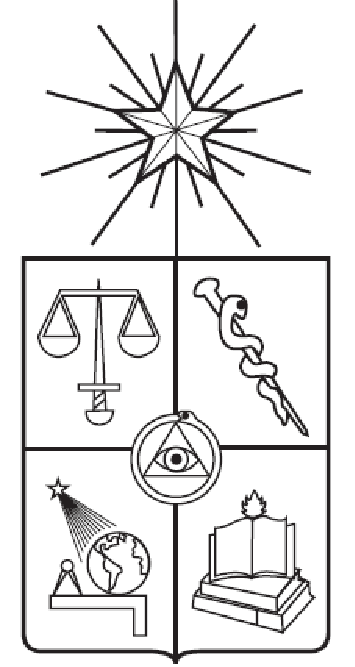
\includegraphics[width=1.5cm]{uchile3}
	\hspace{-0.2cm}
	\begin{tabular}{l}
		\COREwriteheaderitemsc[~\\]{\nombreuniversidad}
		\COREwriteheaderitemsc[~\\]{\nombrefacultad}
		\COREwriteheaderitemsc[~\\]{\departamentouniversidad}
		\vspace*{1cm}\mbox{}
	\end{tabular}
	\vfill
	\begin{center}
		\fontsize{8mm}{9mm}\selectfont
		\textcolor{\portraittitlecolor}{
			\noindent \titulodelinforme ~ \\
		}
		\vspace*{0.5cm}
		\Large{\noindent \textcolor{\portraittitlecolor}{\temaatratar}} ~ \\
		\vspace*{1cm}
		\footnotesize{\codigodelcurso\ - \nombredelcurso} ~ \\
		\vspace*{1.4cm}
	\end{center}
	\vfill
	\begin{center}
		\noindent \normalsize{\tablaintegrantes}
	\end{center}
}{
\ifthenelse{\equal{\portraitstyle}{style6}}{
	\setpagemargincm{\pagemarginleft}{\pagemargintop}{\pagemarginright}{\pagemarginbottom}
	\thispagestyle{empty}
	\begin{wrapfigure}{l}{0.3\textwidth}
		\vspace{-0.69cm}
		\noindent \hspace{-1.10cm} 
\includegraphics[scale=1.35]{fcfm2}
	\end{wrapfigure}
	\def\COREstylefirstmargin {-2.2cm}
	\ifthenelse{\equal{\departamentouniversidad}{\xspace}}{}{
		\hspace*{0.05cm}
		\noindent \textsc{\color{red} \hspace{\COREstylefirstmargin} \departamentouniversidad} ~ \\
		\def\COREstylefirstmargin {-1.6cm}
	}
	\ifthenelse{\equal{\nombrefacultad}{\xspace}}{}{
		\hspace*{0.05cm}
		\noindent \textsc{\color{dkgray} \hspace{\COREstylefirstmargin} \nombrefacultad} ~ \\
		\def\COREstylefirstmargin {-1.6cm}
	}
	\ifthenelse{\equal{\nombreuniversidad}{\xspace}}{}{
		\hspace*{0.05cm}
		\noindent \textsc{\color{dkgray} \hspace{\COREstylefirstmargin} \nombreuniversidad} ~ \\
		\def\COREstylefirstmargin {-1.6cm}
	}
	\ifthenelse{\equal{\nombredelcurso}{\xspace}}{}{
		\hspace*{0.05cm}
		\noindent \textsc{\color{dkgray} \hspace{\COREstylefirstmargin} \codigodelcurso \nombredelcurso} ~ \\
		\def\COREstylefirstmargin {-1.6cm}
	}
	\vfill
	\begin{center}
		\vspace*{0.5cm}
		{\color{dkgray} \Large \textbf{\MakeUppercase{\temaatratar}}} ~ \\
		\noindent \rule{\linewidth}{0.3mm} ~ \\
		\Huge \textup \bfseries \textsc{\textcolor{\portraittitlecolor}{\titulodelinforme}} ~ \\
		\noindent \rule{\linewidth}{0.3mm} ~ \\
	\end{center}
	\begin{minipage}{.5\textwidth}
		~
	\end{minipage}
	\vfill
	\begin{minipage}{1.0\textwidth}
		\begin{flushright}
			\noindent \tablaintegrantes
		\end{flushright}
	\end{minipage}
}{
\ifthenelse{\equal{\portraitstyle}{style7}}{
	\setpagemargincm{\pagemarginleft}{\pagemargintop}{\pagemarginright}{\pagemarginbottom}
	\thispagestyle{empty}
	\begin{center}
		\vspace*{-1.5cm}
		\includegraphics[scale=\imagendepartamentoescala]{\imagendepartamento}
		\hspace*{-0.15cm}
		\begin{tabular}{l}
			\vspace*{0.26cm}\mbox{} ~ \\
			\COREwriteheaderitemsc{\nombreuniversidad}
			\COREwriteheaderitemsc{\nombrefacultad}
			\COREwriteheaderitemsc{\departamentouniversidad}
			\vspace*{1.25cm}\mbox{}
		\end{tabular}
	\end{center}
	\vfill
	\begin{center}
		\noindent \rule{\textwidth}{0.4mm} \\ \vspace{0.3cm}
		{\huge \textcolor{\portraittitlecolor}{\titulodelinforme} \vspace{0.2cm} ~ \\}
		\noindent \rule{\textwidth}{0.4mm} ~ \\ \vspace{0.40cm}
		{\large \textcolor{\portraittitlecolor}{\temaatratar} ~ \\}
	\end{center}
	\vfill
	\noindent
	\begin{minipage}{1.0\textwidth}
		\begin{flushright}
			\scshape{\tablaintegrantes}
		\end{flushright}
	\end{minipage}
}{
\ifthenelse{\equal{\portraitstyle}{style8}}{
	\setpagemargincm{\pagemarginleft}{\pagemargintop}{\pagemarginright}{\pagemarginbottom}
	\thispagestyle{empty}
	\begin{center}
		\vspace*{-1.0cm}
		\begin{tabular}{c}
			\includegraphics[scale=\imagendepartamentoescala]{\imagendepartamento} \vspace{0.5cm} ~ \\
			\COREwriteheaderitemsc{\nombreuniversidad}
			\COREwriteheaderitemsc{\nombrefacultad}
			\COREwriteheaderitemsc{\departamentouniversidad}
		\end{tabular}
	\end{center}
	\vfill
	\begin{center}
		\noindent \rule{\textwidth}{0.4mm} \\ \vspace{0.3cm}
		{\huge \textcolor{\portraittitlecolor}{\titulodelinforme} \vspace{0.2cm} ~ \\}
		\noindent \rule{\textwidth}{0.4mm} ~ \\ \vspace{0.40cm}
		{\large \textcolor{\portraittitlecolor}{\temaatratar} ~ \\}
	\end{center}
	\vfill
	\noindent
	\begin{minipage}{1.0\textwidth}
		\begin{flushright}
			\scshape{\tablaintegrantes}
		\end{flushright}
	\end{minipage}
}{
\ifthenelse{\equal{\portraitstyle}{style9}}{
	\setpagemargincm{\pagemarginleft}{\pagemargintop}{\pagemarginright}{\pagemarginbottom}
	\thispagestyle{empty}
	\noindent \includegraphics[scale=\imagendepartamentoescala]{\imagendepartamento}
	\vfill
	\begin{center}
		\noindent \rule{\textwidth}{0.4mm} \\ \vspace{0.3cm}
		{\huge \textcolor{\portraittitlecolor}{\titulodelinforme} \vspace{0.2cm} \\}
		\noindent \rule{\textwidth}{0.4mm} \\ \vspace{0.35cm}
		{\large \textcolor{\portraittitlecolor}{\temaatratar} \\}
	\end{center}
	\vfill
	\begin{center}
		\begin{tabular}{c}
			\COREwriteheaderitemsc{\nombreuniversidad}
			\COREwriteheaderitemsc{\nombrefacultad}
			\COREwriteheaderitemsc{\departamentouniversidad}
		\end{tabular}
	\end{center}
	\vfill
	\begin{center}
		\indent \scshape{\tablaintegrantes}
	\end{center}
}{
\ifthenelse{\equal{\portraitstyle}{style10}}{
	\setpagemargincm{\pagemarginleft}{\pagemargintop}{\pagemarginright}{\pagemarginbottom}
	\thispagestyle{empty}
	~ \\
	\vfill
	\begin{center}
		\ifthenelse{\equal{\nombreuniversidad}{\xspace}}{
			\noindent {\large \textsc{\departamentouniversidad}}
		}{
			\noindent {\large \textsc{\nombreuniversidad, \departamentouniversidad}}
		}
		\vspace{1.0cm}
	\end{center}
	\vfill
	\begin{center}
		\ifthenelse{\equal{\nombredelcurso}{\xspace}}{}{
			\noindent {\large \scshape{\nombredelcurso}} \vspace{0.5cm} ~ \\
		}
		\ifthenelse{\equal{\codigodelcurso}{\xspace}}{}{
			\noindent {\large \scshape{\codigodelcurso}} \vspace{0.5cm} ~ \\
		}
		\noindent \rule{\textwidth}{0.4mm} \\ \vspace{0.3cm}
		{\huge \bfseries \textcolor{\portraittitlecolor}{\titulodelinforme} \vspace{0.2cm} \\}
		\noindent \rule{\textwidth}{0.4mm} \\ \vspace{2.5cm}
	\end{center}
	\vfill
	\begin{center}
		\indent \tablaintegrantes
	\end{center}
	\vfill
	~ \\
}{
\ifthenelse{\equal{\portraitstyle}{style11}}{
	\setpagemargincm{\pagemarginleft}{\pagemargintop}{\pagemarginright}{\pagemarginbottom}
	\thispagestyle{empty}
	\begin{center}
		\vspace*{-1.0cm}
		\ifthenelse{\equal{\nombreuniversidad}{\xspace}}{}{
			\scshape{\nombreuniversidad} ~ \\
		}
		\ifthenelse{\equal{\nombrefacultad}{\xspace}}{}{
			\scshape{\nombrefacultad} ~ \\
		}
		\ifthenelse{\equal{\departamentouniversidad}{\xspace}}{}{
			\scshape{\departamentouniversidad}
		}
	\end{center}
	\vfill
	\begin{center}
		{\setstretch{1.2} \fontsize{21pt}{22pt} \selectfont \textcolor{\portraittitlecolor}{\scshape{\titulodelinforme}} \vspace{0.5cm}} ~ \\
		{\fontsize{13pt}{10pt} \selectfont \textcolor{\portraittitlecolor}{\scshape{\temaatratar}}}
	\end{center}
	\vfill
	\begin{center}
		\indent \tablaintegrantes
	\end{center}
}{
\ifthenelse{\equal{\portraitstyle}{style12}}{
	\setpagemargincm{\pagemarginleft}{\pagemargintop}{\pagemarginright}{\pagemarginbottom}
	\thispagestyle{empty}
	\begin{center}
		\vspace*{-1.0cm}
		\includegraphics[scale=\imagendepartamentoescala]{\imagendepartamento}
	\end{center}
	\vfill
	\begin{center}
		{\bf \Huge \scshape{\textcolor{\portraittitlecolor}{\titulodelinforme}} \vspace{0.3cm}} \\
		{\bf \Large \textcolor{\portraittitlecolor}{\temaatratar}}
	\end{center}
	\vfill
	\begin{flushright}
		\noindent \tablaintegrantes
	\end{flushright}
	\vspace{0.5cm}
	\noindent \rule{\textwidth}{0.4mm}
	\begin{center}
		\ifthenelse{\equal{\nombreuniversidad}{\xspace}}{
			\scshape{\nombrefacultad} \\
		}{
			\scshape{\nombreuniversidad, \nombrefacultad} \\
		}
		\scshape{\departamentouniversidad}
	\end{center}
}{
\ifthenelse{\equal{\portraitstyle}{style13}}{
	\setpagemargincm{\pagemarginleft}{\pagemargintop}{\pagemarginright}{\pagemarginbottom}
	\thispagestyle{empty}
	\noindent
	\vspace*{-1.5cm}
	\begin{flushleft}
		\begin{minipage}{0.65\textwidth}
			\ifthenelse{\equal{\nombreuniversidad}{\xspace}}{
				{\fontsize{3.5mm}{0.5mm} \selectfont \noindent \textsf{\nombrefacultad}} ~ \\
			}{
				{\fontsize{3.5mm}{0.5mm} \selectfont \noindent \textsf{\nombreuniversidad, \nombrefacultad}} ~ \\
			}
			\noindent {\fontsize{3.0mm}{0.5mm} \selectfont \textsf{\departamentouniversidad} \vspace{-0.2cm}} ~ \\
			\noindent \textcolor{gray}{\rule{\textwidth}{0.3mm}}
		\end{minipage}
	\end{flushleft}
	\vspace*{-2.15cm}
	\begin{flushright}
		\begin{minipage}{0.3\textwidth}
			\noindent \includegraphics[width=1.0\textwidth]{\imagendepartamento}
		\end{minipage}
	\end{flushright}
	\vfill
	\begin{center}
		\begin{minipage}{0.9\textwidth}
			\begin{framed}
				\LARGE
				\vspace{1cm}
				\centering \textcolor{\portraittitlecolor}{\textbf{\titulodelinforme}}
				\vspace{1cm}
			\end{framed}
		\end{minipage}
	\end{center}
	\vfill
	\begin{flushright}
		\noindent \textsf{\tablaintegrantes}
	\end{flushright}
}{
\ifthenelse{\equal{\portraitstyle}{style14}}{
	\setpagemargincm{\pagemarginleft}{\pagemargintop}{\pagemarginright}{\pagemarginbottom}
	\thispagestyle{empty}
	\noindent
	\begin{flushleft}
		\vspace*{-1.0cm}
		\noindent \includegraphics[scale=\imagendepartamentoescala]{\imagendepartamento} \\
	\end{flushleft}
	\vfill
	{\bf \huge \noindent \textcolor{\portraittitlecolor}{\textsf{\MakeUppercase{\titulodelinforme}} \vspace*{0.05cm}}} \\
	{\bf \large \noindent \textcolor{\portraittitlecolor}{\textsf{\MakeUppercase{\temaatratar}}}} \\
	\vfill
	\begin{flushright}
		\noindent \textsf{\tablaintegrantes}
	\end{flushright}
}{
\ifthenelse{\equal{\portraitstyle}{style15}}{
	\setpagemargincm{\pagemarginleft}{\pagemargintop}{\pagemarginright}{\pagemarginbottom}
	\thispagestyle{empty}
	\checkextravarexist{\headerimageA}{Defina la imagen extra de la portada en el archivo lib/page/portrait-config.tex (VERSION NORMAL) o bien en el bloque PORTADA (VERSION COMPACTA)}
	\checkextravarexist{\headerimagescaleA}{Defina la escala de la imagen extra de la portada en el archivo lib/page/portrait-config.tex (VERSION NORMAL) o bien en el bloque PORTADA (VERSION COMPACTA)}
	\vspace*{-1.5cm}
	\noindent \begin{minipage}{0.8\textwidth}
		\noindent \begin{minipage}{0.22\textwidth}
			
\includegraphics[scale=1.0]{fcfm2} \\
		\end{minipage}
		\begin{minipage}{0.6\textwidth}
			\begin{flushleft}
				\textsc{
				\begin{tabular}{l}
					\ifthenelse{\equal{\nombreuniversidad}{\xspace}}{}{
						{\small \nombreuniversidad} ~ \\
					}
					\ifthenelse{\equal{\nombrefacultad}{\xspace}}{}{
						{\small \nombrefacultad} ~ \\
					}
					\ifthenelse{\equal{\departamentouniversidad}{\xspace}}{}{
						{\small \departamentouniversidad}
					}
				\end{tabular}
				}
			\end{flushleft}
		\end{minipage}
	\end{minipage}
	\noindent \begin{minipage}{0.2\textwidth}
		\begin{flushright}
			\ifthenelse{\isundefined{\headerimageA}}{}{
				\ifthenelse{\isundefined{\headerimagescaleA}}{}{
					\noindent \includegraphics[scale=\headerimagescaleA]{\headerimageA} \\
				}
			}
		\end{flushright}
	\end{minipage}
	\vfill
	\begin{center}
		{\fontsize{25pt}{15pt} \selectfont \textcolor{\portraittitlecolor}{\textbf{\titulodelinforme}} \vspace{0.7cm}} \\
		{\Large \textcolor{\portraittitlecolor}{\temaatratar}}
	\end{center}
	\vfill
	\begin{center}
		\noindent \tablaintegrantes
	\end{center}
}{
\ifthenelse{\equal{\portraitstyle}{style16}}{
	\setpagemargincm{\pagemarginleft}{\pagemargintop}{\pagemarginright}{\pagemarginbottom}
	\checkextravarexist{\portraitbackgroundimageB}{[portrait-style16] Defina el fondo de la portada en el archivo lib/page/portrait-config.tex (VERSION NORMAL) o bien en el bloque PORTADA (VERSION COMPACTA)}
	\checkextravarexist{\portraitbackgroundcolorB}{[portrait-style16] Defina el color del bloque del titulo de la portada en el archivo lib/page/portrait-config.tex (VERSION NORMAL) o bien en el bloque PORTADA (VERSION COMPACTA)}
	\begingroup
		\thispagestyle{empty}
		\begin{tikzpicture}[remember picture,overlay]
			\node[inner sep=0pt] (background) at (current page.center) {\includegraphics[width=\paperwidth]{\portraitbackgroundimageB}};
			\draw (current page.center) node [fill=\portraitbackgroundcolorB!30!white,fill opacity=0.6,text opacity=1,inner sep=1cm]{\Huge\centering\bfseries\sffamily\parbox[c][][t]{\paperwidth}{
					\centering \textcolor{\portraittitlecolor}{\titulodelinforme} \\ [10pt]
					{\Large \textcolor{\portraittitlecolor}{\temaatratar}} \\ [25pt]
					{\huge \autordeldocumento}}};
		\end{tikzpicture}
		\vfill
	\endgroup
}{
\ifthenelse{\equal{\portraitstyle}{style17}}{
	\setpagemargincm{\pagemarginleft}{\firstpagemargintop}{\pagemarginright}{\pagemarginbottom}
	\pagestyle{fancy}
	\checkextravarexist{\portraitimageC}{[portrait-style17] Defina la imagen de la portada en el archivo lib/page/portrait-config.tex (VERSION NORMAL) o bien en el bloque PORTADA (VERSION COMPACTA)}
	\checkextravarexist{\portraitimageboxedC}{[portrait-style17] Defina si la imagen de la portada se encierra en un recuadro en el archivo lib/page/portrait-config.tex (VERSION NORMAL) o bien en el bloque PORTADA (VERSION COMPACTA)}
	\checkextravarexist{\portraitimageboxedwidthC}{[portrait-style17] Defina el grosor del recuadro de la imagen de la portada en el archivo lib/page/portrait-config.tex (VERSION NORMAL) o bien en el bloque PORTADA (VERSION COMPACTA)}
	\checkextravarexist{\portraitimagewidthC}{[portrait-style17] Defina los parametros de la imagen de la portada en el archivo lib/page/portrait-config.tex (VERSION NORMAL) o bien en el bloque PORTADA (VERSION COMPACTA)}
	\fancyhf{}
	\fancyhead[L]{
		\COREwriteheaderitem{\nombreuniversidad}
		\COREwriteheaderitem{\nombrefacultad}
		\COREwriteheaderitem{\departamentouniversidad}
		\vspace{-\baselineskip}
	}
	\fancyhead[R]{
		\includegraphics[scale=\imagendepartamentoescala]{\imagendepartamento}
		\hspace{-0.255cm}
		\vspace{-0.20cm}
	}
	~ \\
	\vfill
	\begin{center}
		\textcolor{\portraittitlecolor}{
			{\noindent \Huge{\titulodelinforme} \vspace{0.5cm}} ~ \\
			{\noindent \large{\temaatratar}}
		}
	\end{center}
	~ \\
	\ifthenelse{\equal{\portraitimageboxedC}{true}}{
		\insertimageboxed{\portraitimageC}{width=\portraitimagewidthC}{\portraitimageboxedwidthC}{}
	}{
		\insertimage{\portraitimageC}{width=\portraitimagewidthC}{}
	}
	~ \\
	\vfill
	\noindent
	\begin{minipage}{1.0\textwidth}
		\begin{flushright}
			\tablaintegrantes
		\end{flushright}
	\end{minipage}
}{
\ifthenelse{\equal{\portraitstyle}{style18}}{
	\setpagemargincm{\pagemarginleft}{\firstpagemargintop}{\pagemarginright}{\pagemarginbottom}
	\pagestyle{fancy}
	\checkextravarexist{\portraitimageD}{[portrait-style18] Defina la imagen de la portada en el archivo lib/page/portrait-config.tex (VERSION NORMAL) o bien en el bloque PORTADA (VERSION COMPACTA)}
	\checkextravarexist{\portraitimageboxedD}{[portrait-style18] Defina si la imagen de la portada se encierra en un recuadro en el archivo lib/page/portrait-config.tex (VERSION NORMAL) o bien en el bloque PORTADA (VERSION COMPACTA)}
	\checkextravarexist{\portraitimageboxedwidthD}{[portrait-style18] Defina el grosor del recuadro de la imagen de la portada en el archivo lib/page/portrait-config.tex (VERSION NORMAL) o bien en el bloque PORTADA (VERSION COMPACTA)}
	\checkextravarexist{\portraitimagewidthD}{[portrait-style18] Defina los parametros de la imagen de la portada en el archivo lib/page/portrait-config.tex (VERSION NORMAL) o bien en el bloque PORTADA (VERSION COMPACTA)}
	\fancyhf{}
	\fancyhead[L]{
		\COREwriteheaderitem{\nombreuniversidad}
		\COREwriteheaderitem{\nombrefacultad}
		\COREwriteheaderitem{\departamentouniversidad}
		\vspace{-\baselineskip}
	}
	\fancyhead[R]{
		\includegraphics[scale=\imagendepartamentoescala]{\imagendepartamento}
		\hspace{-0.255cm}
		\vspace{-0.20cm}
	}
	~ \\
	\ifthenelse{\equal{\portraitimageboxedD}{true}}{
		\insertimageboxed{\portraitimageD}{width=\portraitimagewidthD}{\portraitimageboxedwidthD}{}
	}{
		\insertimage{\portraitimageD}{width=\portraitimagewidthD}{}
	}
	\vfill
	\begin{center}
		\textcolor{\portraittitlecolor}{
			{\noindent \Huge{\titulodelinforme} \vspace{0.5cm}} ~ \\
			{\noindent \large{\temaatratar}}
		}
	\end{center}
	\vfill
	\noindent
	\begin{minipage}{1.0\textwidth}
		\begin{flushright}
			\tablaintegrantes
		\end{flushright}
	\end{minipage}
}{
\ifthenelse{\equal{\portraitstyle}{style19}}{
	\setpagemargincm{\pagemarginleft}{\pagemargintop}{\pagemarginright}{\pagemarginbottom}
	\thispagestyle{empty}
	\vspace*{0cm}
	\begin{center}
		\noindent \rule{\textwidth}{0.4mm} \\ \vspace{0.3cm}
		{\huge \bfseries \textcolor{\portraittitlecolor}{\titulodelinforme} \vspace{0.2cm} \\}
		\noindent \rule{\textwidth}{0.4mm}
	\end{center}
	~ \\
	\begin{center}
		\noindent {\large \scshape{\codigodelcurso} \large \scshape{\nombredelcurso}} \vspace{0.5cm} ~ \\
		\ifthenelse{\equal{\nombreuniversidad}{\xspace}}{
			\noindent {\large \textsc{\departamentouniversidad}}
		}{
			\noindent {\large \textsc{\nombreuniversidad, \departamentouniversidad}}
		}
		\vspace{1.0cm}
	\end{center}
	\vfill
	\begin{center}
		\indent \tablaintegrantes
	\end{center}
	~ \\
}{
\ifthenelse{\equal{\portraitstyle}{style20}}{
	\setpagemargincm{\pagemarginleft}{\pagemargintop}{\pagemarginright}{\pagemarginbottom}
	\thispagestyle{empty}
	{\raggedleft	
	\rule{1pt}{\textheight}
	\hspace{0.05\textwidth}
	\parbox[b]{0.75\textwidth}{
		{\Huge\bfseries \textcolor{\portraittitlecolor}{\titulodelinforme}}\\[2\baselineskip]
		{\large\textit{\textcolor{\portraittitlecolor}{\temaatratar}}}\\[4\baselineskip]
		\vspace*{2cm}
		{\textsc{
		\begin{flushleft}
			\noindent\tablaintegrantes
		\end{flushleft}
		}}
		\vspace*{\portraitverticalspaceE}
		{\noindent \nombreuniversidad ~\\
		\nombrefacultad ~\\
		\departamentouniversidad}\\[\baselineskip]
	}}
}{
\ifthenelse{\equal{\portraitstyle}{\bgtemplatetestcode}}{
	\setpagemargincm{\pagemarginleft}{\pagemargintop}{\pagemarginright}{\pagemarginbottom}
	\pagestyle{empty}
	\pagecolor{lbrown}
	\begin{center}
		\vspace*{-1.0cm}
		\ifthenelse{\equal{\nombreuniversidad}{\xspace}}{}{
			\scshape{\nombreuniversidad} ~ \\
		}
		\ifthenelse{\equal{\nombrefacultad}{\xspace}}{}{
			\scshape{\nombrefacultad} ~ \\
		}
		\ifthenelse{\equal{\departamentouniversidad}{\xspace}}{}{
			\scshape{\departamentouniversidad}
		}
	\end{center}
	~ \\
	\begin{center}
		\bgtemplatetestimg
	\end{center}
	\begin{center}
		\vspace*{-6cm}
		{\setstretch{1.2} \fontsize{25pt}{22pt} \selectfont \textcolor{\portraittitlecolor}{\scshape{\titulodelinforme}} \vspace{0.5cm}} \\
		{\fontsize{15pt}{10pt} \selectfont \textcolor{\portraittitlecolor}{\scshape{\temaatratar}}}
	\end{center}
	\vfill
	\begin{flushright}
		\noindent \tablaintegrantes
	\end{flushright}
	\newpage
	\pagecolor{\colorpage}
}{
	\throwbadconfigondoc{Estilo de portada incorrecto}{\portraitstyle}{style1 .. style20}}}}}}}}}}}}}}}}}}}}}
}
\ifthenelse{\equal{\addemptypagetwosides}{true}}{
	\newpage
	\null
	\thispagestyle{empty}
	\renewcommand{\thepage}{}
	\newpage}{
}
 % Se puede borrar

% CONFIGURACIÓN DE PÁGINA Y ENCABEZADOS
% Template:     Informe/Reporte LaTeX
% Documento:    Configuración de página
% Versión:      6.8.2 (11/04/2020)
% Codificación: UTF-8
%
% Autor: Pablo Pizarro R.
%        Facultad de Ciencias Físicas y Matemáticas
%        Universidad de Chile
%        pablo@ppizarror.com
%
% Manual template: [https://latex.ppizarror.com/informe]
% Licencia MIT:    [https://opensource.org/licenses/MIT]

\newpage
\ifthenelse{\equal{\predocpageromannumber}{true}}{
	\ifthenelse{\equal{\predocpageromanupper}{true}}{
		\pagenumbering{Roman}
	}{
		\pagenumbering{roman}
	}}{
	\pagenumbering{arabic}
}
\setcounter{page}{1}
\setcounter{footnote}{0}
\setpagemargincm{\pagemarginleft}{\pagemargintop}{\pagemarginright}{\pagemarginbottom}
\def\arraystretch {\tablepaddingv}
\setlength{\tabcolsep}{\tablepaddingh em}
\ifthenelse{\equal{\pointdecimal}{true}}{
	\decimalpoint}{
}
\renewcommand{\appendixname}{\nomltappendixsection}
\renewcommand{\appendixpagename}{\nameappendixsection}
\renewcommand{\appendixtocname}{\nameappendixsection}
\renewcommand{\contentsname}{\nomltcont}
\renewcommand{\figurename}{\nomltwfigure}
\renewcommand{\listfigurename}{\nomltfigure}
\renewcommand{\listtablename}{\nomlttable}
\renewcommand{\lstlistingname}{\nomltwsrc}
\renewcommand{\lstlistlistingname}{\nomltsrc}
\renewcommand{\refname}{\namereferences}
\renewcommand{\bibname}{\namereferences}
\renewcommand{\tablename}{\nomltwtable}
\sectionfont{\color{\titlecolor} \fontsizetitle \styletitle \selectfont}
\subsectionfont{\color{\subtitlecolor} \fontsizesubtitle \stylesubtitle \selectfont}
\subsubsectionfont{\color{\subsubtitlecolor} \fontsizesubsubtitle \stylesubsubtitle \selectfont}
\titleformat{\subsubsubsection}{\color{\ssstitlecolor} \normalfont \fontsizessstitle \stylessstitle}{\thesubsubsubsection}{1em}{}
\titlespacing*{\subsubsubsection}{0pt}{3.25ex plus 1ex minus .2ex}{1.5ex plus .2ex}
\fancyheadoffset{0pt}
\def\hfheaderimagesizeA {1.2}
\ifthenelse{\equal{\hfstyle}{style1}}{
	\pagestyle{fancy}
	\newcommand{\COREstyledefinition}{
		\fancyhf{}
		\ifthenelse{\equal{\disablehfrightmark}{false}}{
			\fancyhead[L]{\nouppercase{\rightmark}}
		}{}
		\fancyhead[R]{\small \thepage}
		\ifthenelse{\equal{\hfwidthwrap}{true}}{
			\fancyfoot[L]{
				\begin{minipage}[t]{\hfwidthtitle\linewidth}
					\begin{flushleft}
						\small \textit{\titulodelinforme}
					\end{flushleft}
				\end{minipage}
			}
			\fancyfoot[R]{
				\begin{minipage}[t]{\hfwidthcourse\linewidth}
					\begin{flushright}
						\small \textit{\codigodelcurso \nombredelcurso}
					\end{flushright}
				\end{minipage}
			}
		}{
			\fancyfoot[L]{\small \textit{\titulodelinforme}}
			\fancyfoot[R]{\small \textit{\codigodelcurso \nombredelcurso}}
		}
		\renewcommand{\headrulewidth}{0.5pt}
		\renewcommand{\footrulewidth}{0.5pt}
	}
	\renewcommand{\sectionmark}[1]{\markboth{#1}{}}
	\COREstyledefinition
}{
\ifthenelse{\equal{\hfstyle}{style2}}{
	\pagestyle{fancy}
	\newcommand{\COREstyledefinition}{
		\fancyhf{}
		\ifthenelse{\equal{\disablehfrightmark}{false}}{
			\fancyhead[L]{\nouppercase{\rightmark}}
		}{}
		\fancyhead[R]{\small \thepage}
		\ifthenelse{\equal{\hfwidthwrap}{true}}{
			\fancyfoot[L]{
				\begin{minipage}[t]{\hfwidthtitle\linewidth}
					\begin{flushleft}
						\small \textit{\titulodelinforme}
					\end{flushleft}
				\end{minipage}
			}
			\fancyfoot[R]{
				\begin{minipage}[t]{\hfwidthcourse\linewidth}
					\begin{flushright}
						\small \textit{\codigodelcurso \nombredelcurso}
					\end{flushright}
				\end{minipage}
			}
		}{
			\fancyfoot[L]{\small \textit{\titulodelinforme}}
			\fancyfoot[R]{\small \textit{\codigodelcurso \nombredelcurso}}
		}
		\renewcommand{\headrulewidth}{0.5pt}
		\renewcommand{\footrulewidth}{0pt}
	}
	\renewcommand{\sectionmark}[1]{\markboth{#1}{}}
	\COREstyledefinition
}{
\ifthenelse{\equal{\hfstyle}{style3}}{
	\pagestyle{fancy}
	\newcommand{\COREstyledefinition}{
		\fancyhf{}
		\ifthenelse{\equal{\hfwidthwrap}{true}}{
			\fancyhead[L]{
				\begin{minipage}[t]{\hfwidthtitle\linewidth}
					\begin{flushleft}
						\small \textit{\codigodelcurso \nombredelcurso}
					\end{flushleft}
				\end{minipage}
			}
		}{
			\fancyhead[L]{\small \textit{\codigodelcurso \nombredelcurso}}
		}
		\fancyhead[R]{
			\includegraphics[width=\hfheaderimagesizeA cm]{\imagendepartamento}
			\vspace{-0.15cm}
		}
		\fancyfoot[C]{\thepage}
		\renewcommand{\headrulewidth}{0.5pt}
		\renewcommand{\footrulewidth}{0pt}
	}
	\COREstyledefinition
}{
\ifthenelse{\equal{\hfstyle}{style4}}{
	\pagestyle{fancy}
	\newcommand{\COREstyledefinition}{
		\fancyhf{}
		\ifthenelse{\equal{\disablehfrightmark}{false}}{
			\fancyhead[L]{\nouppercase{\rightmark}}
		}{}
		\fancyhead[R]{}
		\fancyfoot[C]{\small \thepage}
		\renewcommand{\headrulewidth}{0.5pt}
		\renewcommand{\footrulewidth}{0pt}
	}
	\renewcommand{\sectionmark}[1]{\markboth{#1}{}}
	\COREstyledefinition
}{
\ifthenelse{\equal{\hfstyle}{style5}}{
	\pagestyle{fancy}
	\newcommand{\COREstyledefinition}{
		\fancyhf{}
		\ifthenelse{\equal{\hfwidthwrap}{true}}{
			\fancyhead[L]{
				\begin{minipage}[t]{\hfwidthcourse\linewidth}
					\begin{flushleft}
						\codigodelcurso \nombredelcurso
					\end{flushleft}
				\end{minipage}
			}
			\ifthenelse{\equal{\disablehfrightmark}{false}}{
				\fancyhead[R]{
					\begin{minipage}[t]{\hfwidthtitle\linewidth}
						\begin{flushright}
							\nouppercase{\rightmark}
						\end{flushright}
					\end{minipage}
				}
			}{}
		}{
			\fancyhead[L]{\codigodelcurso \nombredelcurso}
			\ifthenelse{\equal{\disablehfrightmark}{false}}{
				\fancyhead[R]{\nouppercase{\rightmark}}
			}{}
		}
		\fancyfoot[L]{\departamentouniversidad, \nombreuniversidad}
		\fancyfoot[R]{\small \thepage}
		\renewcommand{\headrulewidth}{0pt}
		\renewcommand{\footrulewidth}{0pt}
	}
	\renewcommand{\sectionmark}[1]{\markboth{#1}{}}
	\COREstyledefinition
}{
\ifthenelse{\equal{\hfstyle}{style6}}{
	\pagestyle{fancy}
	\newcommand{\COREstyledefinition}{
		\fancyhf{}
		\fancyfoot[L]{\departamentouniversidad}
		\fancyfoot[C]{\thepage}
		\fancyfoot[R]{\nombreuniversidad}
		\renewcommand{\headrulewidth}{0pt}
		\renewcommand{\footrulewidth}{0pt}
	}
	\setlength{\headheight}{49pt}
	\COREstyledefinition
}{
\ifthenelse{\equal{\hfstyle}{style7}}{
	\pagestyle{fancy}
	\newcommand{\COREstyledefinition}{
		\fancyhf{}
		\fancyfoot[C]{\thepage}
		\renewcommand{\headrulewidth}{0pt}
		\renewcommand{\footrulewidth}{0pt}
	}
	\setlength{\headheight}{49pt}
	\COREstyledefinition
}{
\ifthenelse{\equal{\hfstyle}{style8}}{
	\pagestyle{fancy}
	\newcommand{\COREstyledefinition}{
		\fancyhf{}
		\fancyfoot[R]{\thepage}
		\renewcommand{\headrulewidth}{0pt}
		\renewcommand{\footrulewidth}{0pt}
	}
	\setlength{\headheight}{49pt}
	\COREstyledefinition
}{
\ifthenelse{\equal{\hfstyle}{style9}}{
	\pagestyle{fancy}
	\newcommand{\COREstyledefinition}{
		\fancyhf{}
		\ifthenelse{\equal{\disablehfrightmark}{false}}{
			\fancyhead[L]{\nouppercase{\rightmark}}
		}{}
		\fancyhead[R]{}
		\fancyfoot[L]{\small \textit{\titulodelinforme}}
		\fancyfoot[R]{\small \thepage}
		\renewcommand{\headrulewidth}{0.5pt}
		\renewcommand{\footrulewidth}{0.5pt}
	}
	\renewcommand{\sectionmark}[1]{\markboth{#1}{}}
	\COREstyledefinition
}{
\ifthenelse{\equal{\hfstyle}{style10}}{
	\pagestyle{fancy}
	\newcommand{\COREstyledefinition}{
		\fancyhf{}
		\ifthenelse{\equal{\hfwidthwrap}{true}}{
			\ifthenelse{\equal{\disablehfrightmark}{false}}{
				\fancyhead[L]{
					\begin{minipage}[t]{\hfwidthtitle\linewidth}
						\begin{flushleft}
							\nouppercase{\rightmark}
						\end{flushleft}
					\end{minipage}
				}
			}{}
			\fancyhead[R]{
				\begin{minipage}[t]{\hfwidthcourse\linewidth}
					\begin{flushright}
						\small \textit{\titulodelinforme}
					\end{flushright}
				\end{minipage}
			}
		}{
			\ifthenelse{\equal{\disablehfrightmark}{false}}{
				\fancyhead[L]{\nouppercase{\rightmark}}
			}{}
			\fancyhead[R]{\small \textit{\titulodelinforme}}
		}
		\fancyfoot[L]{}
		\fancyfoot[R]{\small \thepage}
		\renewcommand{\headrulewidth}{0.5pt}
		\renewcommand{\footrulewidth}{0.5pt}
	}
	\renewcommand{\sectionmark}[1]{\markboth{#1}{}}
	\COREstyledefinition
}{
\ifthenelse{\equal{\hfstyle}{style11}}{
	\pagestyle{fancy}
	\newcommand{\COREstyledefinition}{
		\fancyhf{}
		\ifthenelse{\equal{\disablehfrightmark}{false}}{
			\fancyhead[L]{\nouppercase{\rightmark}}
		}{}
		\fancyhead[R]{\small \thepage \nomnpageof \pageref{LastPage}}
		\ifthenelse{\equal{\hfwidthwrap}{true}}{
			\fancyfoot[L]{
				\begin{minipage}[t]{\hfwidthtitle\linewidth}
					\begin{flushleft}
						\small \textit{\titulodelinforme}
					\end{flushleft}
				\end{minipage}
			}
			\fancyfoot[R]{
				\begin{minipage}[t]{\hfwidthcourse\linewidth}
					\begin{flushright}
						\small \textit{\codigodelcurso \nombredelcurso}
					\end{flushright}
				\end{minipage}
			}
		}{
			\fancyfoot[L]{\small \textit{\titulodelinforme}}
			\fancyfoot[R]{\small \textit{\codigodelcurso \nombredelcurso}}
		}
		\renewcommand{\headrulewidth}{0.5pt}
		\renewcommand{\footrulewidth}{0.5pt}
	}
	\renewcommand{\sectionmark}[1]{\markboth{#1}{}}
	\COREstyledefinition
}{
\ifthenelse{\equal{\hfstyle}{style12}}{
	\pagestyle{fancy}
	\newcommand{\COREstyledefinition}{
		\fancyhf{}
		\fancyfoot[L]{\departamentouniversidad}
		\fancyfoot[C]{\thepage \nomnpageof \pageref{LastPage}}
		\fancyfoot[R]{\nombreuniversidad}
		\renewcommand{\headrulewidth}{0pt}
		\renewcommand{\footrulewidth}{0pt}
	}
	\setlength{\headheight}{49pt}
	\COREstyledefinition
}{
\ifthenelse{\equal{\hfstyle}{style13}}{
	\pagestyle{fancy}
	\newcommand{\COREstyledefinition}{
		\fancyhf{}
		\ifthenelse{\equal{\hfwidthwrap}{true}}{
			\fancyhead[L]{
				\begin{minipage}[t]{\hfwidthtitle\linewidth}
					\begin{flushleft}
						\small \textit{\codigodelcurso \nombredelcurso}
					\end{flushleft}
				\end{minipage}
			}
		}{
			\fancyhead[L]{\small \textit{\codigodelcurso \nombredelcurso}}
		}
		\fancyhead[R]{
			\includegraphics[width=\hfheaderimagesizeA cm]{\imagendepartamento}
			\vspace{-0.15cm}
		}
		\fancyfoot[C]{\thepage \nomnpageof \pageref{LastPage}}
		\renewcommand{\headrulewidth}{0.5pt}
		\renewcommand{\footrulewidth}{0pt}
	}
	\COREstyledefinition
}{
\ifthenelse{\equal{\hfstyle}{style14}}{
	\pagestyle{fancy}
	\newcommand{\COREstyledefinition}{
		\fancyhf{}
		\ifthenelse{\equal{\disablehfrightmark}{false}}{
			\fancyhead[L]{\nouppercase{\rightmark}}
		}{}
		\fancyhead[R]{}
		\fancyfoot[C]{\small \thepage \nomnpageof \pageref{LastPage}}
		\renewcommand{\headrulewidth}{0.5pt}
		\renewcommand{\footrulewidth}{0pt}
	}
	\renewcommand{\sectionmark}[1]{\markboth{#1}{}}
	\COREstyledefinition
}{
\ifthenelse{\equal{\hfstyle}{style15}}{
	\pagestyle{fancy}
	\newcommand{\COREstyledefinition}{
		\fancyhf{}
		\ifthenelse{\equal{\disablehfrightmark}{false}}{
			\fancyhead[L]{\nouppercase{\rightmark}}
		}{}
		\fancyhead[R]{}
		\fancyfoot[L]{
			\small \codigodelcurso \nombredelcurso
		}
		\fancyfoot[R]{
			\small \thepage
		}
		\renewcommand{\headrulewidth}{0.5pt}
		\renewcommand{\footrulewidth}{0.5pt}
	}
	\renewcommand{\sectionmark}[1]{\markboth{#1}{}}
	\COREstyledefinition
}{
\ifthenelse{\equal{\hfstyle}{style16}}{
	\pagestyle{fancy}
	\newcommand{\COREstyledefinition}{
		\fancyhf{}
		\renewcommand{\headrulewidth}{0pt}
		\renewcommand{\footrulewidth}{0pt}
	}
	\renewcommand{\sectionmark}[1]{\markboth{#1}{}}
	\COREstyledefinition
}{
	\throwbadconfigondoc{Estilo de header-footer incorrecto}{\hfstyle}{style1 .. style16}}}}}}}}}}}}}}}}
}
\fancypagestyle{plain}{
	\fancyheadoffset{0pt}
	\COREstyledefinition
}
\ifthenelse{\equal{\showlinenumbers}{true}}{
	\linenumbers}{
}


% RESUMEN O ABSTRACT
\begin{resumen}
Un circuito eléctrico sencillo se compone de una fuente de poder que es la que entrega la energía a este circuito y la resistencia que es la oposición al movimiento de esta energía. El objetivo es familiarizarse con los conceptos básicos de circuitos eléctricos, esto incluye además, conocer los instrumentos con los que se realizan mediciones en los circuitos eléctricos: amperímetro y voltímetro, cuya finalidad es medir el voltaje y la intensidad de corriente respectivamente. 

Como primera experiencia se busca verificar la ley de Ohm, esta ley consiste en el comportamiento lineal del voltaje en función de la intensidad de corriente, esto se hace a través de la medición del voltaje e intensidad de corriente de un circuito eléctrico usando un amperímetro y voltímetro, no obstante, también se hace prescindiendo de estos instrumentos, esto debido a que el software que se usa para simular el circuito (LTspice) cuenta con sus propias herramientas de medición.

La segunda experiencia es verificar la ley de Kirchhoff las cuales consisten en dos leyes. En primer lugar está la ley de corrientes, que dice que las sumas de intensidades de corriente que entran y salen de un nodo del circuito es 0, la cual se verifica a través de la medición del voltaje y la intensidad de corriente de dos circuitos, uno en serie y otro en paralelo. Y por otro lado, la ley de  voltajes que afirma que la suma de las fuerzas electromotrices es igual a las caídas de voltajes (debido a las resistencias).

Durante la realización de ambas experiencias se pudieron comprobar tanto la ley de Ohm como las leyes de Kirchhoff. Además se instruyó sobre la aplicación de instrumentos de medición como el amperímetro y el voltímetro y también se logró familiarizar con conceptos introductorios de circuitos eléctricos.

%Ohmetro culiao quien te conoce

% ley de OHm
\end{resumen}

% TABLA DE CONTENIDOS - ÍNDICE
% Template:     Informe/Reporte LaTeX
% Documento:    Índice
% Versión:      6.8.2 (11/04/2020)
% Codificación: UTF-8
%
% Autor: Pablo Pizarro R.
%        Facultad de Ciencias Físicas y Matemáticas
%        Universidad de Chile
%        pablo@ppizarror.com
%
% Manual template: [https://latex.ppizarror.com/informe]
% Licencia MIT:    [https://opensource.org/licenses/MIT]

\ifthenelse{\equal{\showindex}{true}}{
	\newpage
	\begingroup
	\sectionfont{\color{\indextitlecolor} \fontsizetitlei \styletitlei \selectfont}
	\ifthenelse{\equal{\addemptypagetwosides}{true}}{
		\checkoddpage
		\ifoddpage
		\else
			\newpage
			\null
			\thispagestyle{empty}
			\newpage
			\addtocounter{page}{-1}
		\fi}{
	}
	\ifthenelse{\equal{\addindextobookmarks}{true}}{
		\belowpdfbookmark{\nomltcont}{contents}}{
	}
	\tocloftpagestyle{fancy}
	\ifthenelse{\equal{\showdotaftersnum}{true}}{
		\def\cftchapaftersnum {.}
		\def\cftsecaftersnum {.}
		\def\cftsubsecaftersnum {.}
		\def\cftsubsubsecaftersnum {.}
		\def\cftsubsubsubsecaftersnum {.}
		\def\cftsecnumwidth {1.9em}
\def\cftsubsecnumwidth {2.57em}
\renewcommand\cftsubsubsecnumwidth{3.35em}
		\setlength{\cftsubsecindent}{1.91em}
\setlength{\cftsubsubsecindent}{4.48em}
		}{
	}
	\renewcommand{\cftdot}{\charnumpageindex}
\def\cftfigaftersnum {\charafterobjectindex\enspace}
\def\cftsubfigaftersnum {\charafterobjectindex\enspace}
\def\cfttabaftersnum {\charafterobjectindex\enspace}
\def\cftlstlistingaftersnum {\charafterobjectindex\enspace}
\def\cftmyindexequationsaftersnum {\charafterobjectindex\enspace}
	\ifthenelse{\equal{\showlinenumbers}{true}}{
		\nolinenumbers}{
	}
	\ifthenelse{\equal{\objectindexindent}{true}}{
\setlength{\cfttabindent}{1.9em}
\setlength{\cftfigindent}{1.9em}
\setlength{\cftsubfigindent}{1.9em}
\setlength{\cftmyindexequationsindent}{1.9em}
\def\cftlstlistingindent {1.9em}
	}{
\setlength{\cfttabindent}{0em}
\setlength{\cftfigindent}{0em}
\setlength{\cftsubfigindent}{0em}
\setlength{\cftmyindexequationsindent}{0em}
\def\cftlstlistingindent {0em}
	}
	\ifthenelse{\equal{\showsectioncaptioncode}{none}}{
\def\cftdefautnumwidthcode {3.0em}
\def\cftdefaultnumwidthromancode {5.25em}
	}{
	\ifthenelse{\equal{\showsectioncaptioncode}{sec}}{
		\def\cftdefautnumwidthcode {3.7em}
		\def\cftdefaultnumwidthromancode {5.75em}
	}{
	\ifthenelse{\equal{\showsectioncaptioncode}{ssec}}{
		\def\cftdefautnumwidthcode {4.4em}
		\def\cftdefaultnumwidthromancode {6.25em}
	}{
	\ifthenelse{\equal{\showsectioncaptioncode}{sssec}}{
		\def\cftdefautnumwidthcode {5.1em}
		\def\cftdefaultnumwidthromancode {6.75em}
	}{
	\ifthenelse{\equal{\showsectioncaptioncode}{ssssec}}{
		\def\cftdefautnumwidthcode {5.8em}
		\def\cftdefaultnumwidthromancode {7.25em}
	}{
	\ifthenelse{\equal{\showsectioncaptioncode}{chap}}{
		\def\cftdefautnumwidthcode {3.0em}
		\def\cftdefaultnumwidthromancode {5.25em}
	}{
		\throwbadconfig{Valor configuracion incorrecto}{\showsectioncaptioncode}{none,chap,sec,ssec,sssec,ssssec}}}}}}
	}
	\ifthenelse{\equal{\showsectioncaptioneqn}{none}}{
\def\cftdefautnumwidtheqn {3.0em}
\def\cftdefaultnumwidthromaneqn {5.25em}
	}{
	\ifthenelse{\equal{\showsectioncaptioneqn}{sec}}{
		\def\cftdefautnumwidtheqn {3.7em}
		\def\cftdefaultnumwidthromaneqn {5.75em}
	}{
	\ifthenelse{\equal{\showsectioncaptioneqn}{ssec}}{
		\def\cftdefautnumwidtheqn {4.4em}
		\def\cftdefaultnumwidthromaneqn {6.25em}
	}{
	\ifthenelse{\equal{\showsectioncaptioneqn}{sssec}}{
		\def\cftdefautnumwidtheqn {5.1em}
		\def\cftdefaultnumwidthromaneqn {6.75em}
	}{
	\ifthenelse{\equal{\showsectioncaptioneqn}{ssssec}}{
		\def\cftdefautnumwidtheqn {5.8em}
		\def\cftdefaultnumwidthromaneqn {7.25em}
	}{
	\ifthenelse{\equal{\showsectioncaptioneqn}{chap}}{
		\def\cftdefautnumwidtheqn {3.0em}
		\def\cftdefaultnumwidthromaneqn {5.25em}
	}{
		\throwbadconfig{Valor configuracion incorrecto}{\showsectioncaptioneqn}{none,chap,sec,ssec,sssec,ssssec}}}}}}
	}
	\ifthenelse{\equal{\showsectioncaptionfig}{none}}{
\def\cftdefautnumwidthfig {3.0em}
\def\cftdefaultnumwidthromanfig {5.25em}
	}{
	\ifthenelse{\equal{\showsectioncaptionfig}{sec}}{
		\def\cftdefautnumwidthfig {3.7em}
		\def\cftdefaultnumwidthromanfig {5.75em}
	}{
	\ifthenelse{\equal{\showsectioncaptionfig}{ssec}}{
		\def\cftdefautnumwidthfig {4.4em}
		\def\cftdefaultnumwidthromanfig {6.25em}
	}{
	\ifthenelse{\equal{\showsectioncaptionfig}{sssec}}{
		\def\cftdefautnumwidthfig {5.1em}
		\def\cftdefaultnumwidthromanfig {6.75em}
	}{
	\ifthenelse{\equal{\showsectioncaptionfig}{ssssec}}{
		\def\cftdefautnumwidthfig {5.8em}
		\def\cftdefaultnumwidthromanfig {7.25em}
	}{
	\ifthenelse{\equal{\showsectioncaptionfig}{chap}}{
		\def\cftdefautnumwidthfig {3.0em}
		\def\cftdefaultnumwidthromanfig {5.25em}
	}{
		\throwbadconfig{Valor configuracion incorrecto}{\showsectioncaptionfig}{none,chap,sec,ssec,sssec,ssssec}}}}}}
	}
	\ifthenelse{\equal{\showsectioncaptiontab}{none}}{
\def\cftdefautnumwidthtab {3.0em}
\def\cftdefaultnumwidthromantab {5.25em}
	}{
	\ifthenelse{\equal{\showsectioncaptiontab}{sec}}{
		\def\cftdefautnumwidthtab {3.7em}
		\def\cftdefaultnumwidthromantab {5.75em}
	}{
	\ifthenelse{\equal{\showsectioncaptiontab}{ssec}}{
		\def\cftdefautnumwidthtab {4.4em}
		\def\cftdefaultnumwidthromantab {6.25em}
	}{
	\ifthenelse{\equal{\showsectioncaptiontab}{sssec}}{
		\def\cftdefautnumwidthtab {5.1em}
		\def\cftdefaultnumwidthromantab {6.75em}
	}{
	\ifthenelse{\equal{\showsectioncaptiontab}{ssssec}}{
		\def\cftdefautnumwidthtab {5.8em}
		\def\cftdefaultnumwidthromantab {7.25em}
	}{
	\ifthenelse{\equal{\showsectioncaptiontab}{chap}}{
		\def\cftdefautnumwidthtab {3.0em}
		\def\cftdefaultnumwidthromantab {5.25em}
	}{
		\throwbadconfig{Valor configuracion incorrecto}{\showsectioncaptiontab}{none,chap,sec,ssec,sssec,ssssec}}}}}}
	}
	\def\cftfignumwidth {\cftdefautnumwidth}
	\def\cfttabnumwidth {\cftdefautnumwidth}
	\def\cftlstlistingnumwidth {\cftdefautnumwidth}
\ifthenelse{\equal{\captionnumcode}{arabic}}{
		\def\cftlstlistingnumwidth {\cftdefautnumwidthcode}
	}{
		\ifthenelse{\equal{\captionnumcode}{roman}}{
			\def\cftlstlistingnumwidth {\cftdefaultnumwidthromancode}
		}{
		\ifthenelse{\equal{\captionnumcode}{Roman}}{
			\def\cftlstlistingnumwidth {\cftdefaultnumwidthromancode}
		}{
			\def\cftlstlistingnumwidth {\cftdefautnumwidthcode}
		}}
	}
\ifthenelse{\equal{\captionnumequation}{arabic}}{
		\def\cftmyindexequationsnumwidth {\cftdefautnumwidtheqn}
	}{
		\ifthenelse{\equal{\captionnumequation}{roman}}{
			\def\cftmyindexequationsnumwidth {\cftdefaultnumwidthromaneqn}
		}{
		\ifthenelse{\equal{\captionnumequation}{Roman}}{
			\def\cftmyindexequationsnumwidth {\cftdefaultnumwidthromaneqn}
		}{
			\def\cftmyindexequationsnumwidth {\cftdefautnumwidtheqn}
		}}
	}
\ifthenelse{\equal{\captionnumfigure}{arabic}}{
		\def\cftfignumwidth {\cftdefautnumwidthfig}
	}{
		\ifthenelse{\equal{\captionnumfigure}{roman}}{
			\def\cftfignumwidth {\cftdefaultnumwidthromanfig}
		}{
			\ifthenelse{\equal{\captionnumfigure}{Roman}}{
				\def\cftfignumwidth {\cftdefaultnumwidthromanfig}
			}{
				\def\cftfignumwidth {\cftdefautnumwidthfig}
			}}
	}
\ifthenelse{\equal{\captionnumtable}{arabic}}{
		\def\cfttabnumwidth {\cftdefautnumwidthtab}
	}{
		\ifthenelse{\equal{\captionnumtable}{roman}}{
			\def\cfttabnumwidth {\cftdefaultnumwidthromantab}
		}{
			\ifthenelse{\equal{\captionnumtable}{Roman}}{
				\def\cfttabnumwidth {\cftdefaultnumwidthromantab}
			}{
				\def\cfttabnumwidth {\cftdefautnumwidthtab}
			}}
	}
\newcommand{\LoIf}{
		\iftotalfigures
			\ifthenelse{\equal{\indexnewpagef}{true}}{\newpage}{}
			\listoffigures
		\fi
	}
\newcommand{\LoIt}{
		\iftotaltables
			\ifthenelse{\equal{\indexnewpaget}{true}}{\newpage}{}
			\listoftables
		\fi
	}
\newcommand{\LoIc}{
		\iftotallstlistings
			\ifthenelse{\equal{\indexnewpagec}{true}}{\newpage}{}
			\lstlistoflistings
		\fi
	}
\newcommand{\LoIe}{
		\iftotaltemplateIndexEquationss
			\ifthenelse{\equal{\indexnewpagee}{true}}{\newpage}{}
			\listofmyindexequations
		\fi
	}
	\ifthenelse{\equal{\showindexofcontents}{true}}{
		\tableofcontents
	}{}
	\ifthenelse{\equal{\indexstyle}{tfce}}{\LoIt\LoIf\LoIc\LoIe}{\ifthenelse{\equal{\indexstyle}{}}{}{\ifthenelse{\equal{\indexstyle}{e}}{\LoIe}{\ifthenelse{\equal{\indexstyle}{c}}{\LoIc}{\ifthenelse{\equal{\indexstyle}{f}}{\LoIf}{\ifthenelse{\equal{\indexstyle}{t}}{\LoIt}{\ifthenelse{\equal{\indexstyle}{ec}}{\LoIe\LoIc}{\ifthenelse{\equal{\indexstyle}{ce}}{\LoIc\LoIe}{\ifthenelse{\equal{\indexstyle}{ef}}{\LoIe\LoIf}{\ifthenelse{\equal{\indexstyle}{fe}}{\LoIf\LoIe}{\ifthenelse{\equal{\indexstyle}{et}}{\LoIe\LoIt}{\ifthenelse{\equal{\indexstyle}{te}}{\LoIt\LoIe}{\ifthenelse{\equal{\indexstyle}{cf}}{\LoIc\LoIf}{\ifthenelse{\equal{\indexstyle}{fc}}{\LoIf\LoIc}{\ifthenelse{\equal{\indexstyle}{ct}}{\LoIc\LoIt}{\ifthenelse{\equal{\indexstyle}{tc}}{\LoIt\LoIc}{\ifthenelse{\equal{\indexstyle}{ft}}{\LoIf\LoIt}{\ifthenelse{\equal{\indexstyle}{tf}}{\LoIt\LoIf}{\ifthenelse{\equal{\indexstyle}{ecf}}{\LoIe\LoIc\LoIf}{\ifthenelse{\equal{\indexstyle}{efc}}{\LoIe\LoIf\LoIc}{\ifthenelse{\equal{\indexstyle}{cef}}{\LoIc\LoIe\LoIf}{\ifthenelse{\equal{\indexstyle}{cfe}}{\LoIc\LoIf\LoIe}{\ifthenelse{\equal{\indexstyle}{fec}}{\LoIf\LoIe\LoIc}{\ifthenelse{\equal{\indexstyle}{fce}}{\LoIf\LoIc\LoIe}{\ifthenelse{\equal{\indexstyle}{ect}}{\LoIe\LoIc\LoIt}{\ifthenelse{\equal{\indexstyle}{etc}}{\LoIe\LoIt\LoIc}{\ifthenelse{\equal{\indexstyle}{cet}}{\LoIc\LoIe\LoIt}{\ifthenelse{\equal{\indexstyle}{cte}}{\LoIc\LoIt\LoIe}{\ifthenelse{\equal{\indexstyle}{tec}}{\LoIt\LoIe\LoIc}{\ifthenelse{\equal{\indexstyle}{tce}}{\LoIt\LoIc\LoIe}{\ifthenelse{\equal{\indexstyle}{eft}}{\LoIe\LoIf\LoIt}{\ifthenelse{\equal{\indexstyle}{etf}}{\LoIe\LoIt\LoIf}{\ifthenelse{\equal{\indexstyle}{fet}}{\LoIf\LoIe\LoIt}{\ifthenelse{\equal{\indexstyle}{fte}}{\LoIf\LoIt\LoIe}{\ifthenelse{\equal{\indexstyle}{tef}}{\LoIt\LoIe\LoIf}{\ifthenelse{\equal{\indexstyle}{tfe}}{\LoIt\LoIf\LoIe}{\ifthenelse{\equal{\indexstyle}{cft}}{\LoIc\LoIf\LoIt}{\ifthenelse{\equal{\indexstyle}{ctf}}{\LoIc\LoIt\LoIf}{\ifthenelse{\equal{\indexstyle}{fct}}{\LoIf\LoIc\LoIt}{\ifthenelse{\equal{\indexstyle}{ftc}}{\LoIf\LoIt\LoIc}{\ifthenelse{\equal{\indexstyle}{tcf}}{\LoIt\LoIc\LoIf}{\ifthenelse{\equal{\indexstyle}{tfc}}{\LoIt\LoIf\LoIc}{\ifthenelse{\equal{\indexstyle}{ecft}}{\LoIe\LoIc\LoIf\LoIt}{\ifthenelse{\equal{\indexstyle}{ectf}}{\LoIe\LoIc\LoIt\LoIf}{\ifthenelse{\equal{\indexstyle}{efct}}{\LoIe\LoIf\LoIc\LoIt}{\ifthenelse{\equal{\indexstyle}{eftc}}{\LoIe\LoIf\LoIt\LoIc}{\ifthenelse{\equal{\indexstyle}{etcf}}{\LoIe\LoIt\LoIc\LoIf}{\ifthenelse{\equal{\indexstyle}{etfc}}{\LoIe\LoIt\LoIf\LoIc}{\ifthenelse{\equal{\indexstyle}{ceft}}{\LoIc\LoIe\LoIf\LoIt}{\ifthenelse{\equal{\indexstyle}{cetf}}{\LoIc\LoIe\LoIt\LoIf}{\ifthenelse{\equal{\indexstyle}{cfet}}{\LoIc\LoIf\LoIe\LoIt}{\ifthenelse{\equal{\indexstyle}{cfte}}{\LoIc\LoIf\LoIt\LoIe}{\ifthenelse{\equal{\indexstyle}{ctef}}{\LoIc\LoIt\LoIe\LoIf}{\ifthenelse{\equal{\indexstyle}{ctfe}}{\LoIc\LoIt\LoIf\LoIe}{\ifthenelse{\equal{\indexstyle}{fect}}{\LoIf\LoIe\LoIc\LoIt}{\ifthenelse{\equal{\indexstyle}{fetc}}{\LoIf\LoIe\LoIt\LoIc}{\ifthenelse{\equal{\indexstyle}{fcet}}{\LoIf\LoIc\LoIe\LoIt}{\ifthenelse{\equal{\indexstyle}{fcte}}{\LoIf\LoIc\LoIt\LoIe}{\ifthenelse{\equal{\indexstyle}{ftec}}{\LoIf\LoIt\LoIe\LoIc}{\ifthenelse{\equal{\indexstyle}{ftce}}{\LoIf\LoIt\LoIc\LoIe}{\ifthenelse{\equal{\indexstyle}{tecf}}{\LoIt\LoIe\LoIc\LoIf}{\ifthenelse{\equal{\indexstyle}{tefc}}{\LoIt\LoIe\LoIf\LoIc}{\ifthenelse{\equal{\indexstyle}{tcef}}{\LoIt\LoIc\LoIe\LoIf}{\ifthenelse{\equal{\indexstyle}{tcfe}}{\LoIt\LoIc\LoIf\LoIe}{\ifthenelse{\equal{\indexstyle}{tfec}}{\LoIt\LoIf\LoIe\LoIc}{\throwbadconfig{Estilo desconocido del indice}{\indexstyle}{tfce,,e,c,f,t,ec,ce,ef,fe,et,te,cf,fc,ct,tc,ft,tf,ecf,efc,cef,cfe,fec,fce,ect,etc,cet,cte,tec,tce,eft,etf,fet,fte,tef,tfe,cft,ctf,fct,ftc,tcf,tfc,ecft,ectf,efct,eftc,etcf,etfc,ceft,cetf,cfet,cfte,ctef,ctfe,fect,fetc,fcet,fcte,ftec,ftce,tecf,tefc,tcef,tcfe,tfec}}}}}}}}}}}}}}}}}}}}}}}}}}}}}}}}}}}}}}}}}}}}}}}}}}}}}}}}}}}}}}}}}}
	\endgroup
	\newpage
	\ifthenelse{\equal{\addemptypagetwosides}{true}}{
		\vfill
		\checkoddpage
		\ifoddpage
			\newpage
			\null
			\thispagestyle{empty}
			\newpage
			\addtocounter{page}{-1}
		\else
		\fi}{
	}
}{}
 % Se puede borrar

% CONFIGURACIONES FINALES
% Template:     Informe/Reporte LaTeX
% Documento:    Configuraciones finales
% Versión:      6.8.2 (11/04/2020)
% Codificación: UTF-8
%
% Autor: Pablo Pizarro R.
%        Facultad de Ciencias Físicas y Matemáticas
%        Universidad de Chile
%        pablo@ppizarror.com
%
% Manual template: [https://latex.ppizarror.com/informe]
% Licencia MIT:    [https://opensource.org/licenses/MIT]

\markboth{}{}
\newpage
\ifthenelse{\equal{\disablehfrightmark}{false}}{
	\ifthenelse{\equal{\hfstyle}{style1}}{
		\fancypagestyle{plain}{\fancyhead[L]{\nouppercase{\leftmark}}}
		\fancyhead[L]{\nouppercase{\leftmark}}}{
	}
	\ifthenelse{\equal{\hfstyle}{style2}}{
		\fancypagestyle{plain}{\fancyhead[L]{\nouppercase{\leftmark}}}
		\fancyhead[L]{\nouppercase{\leftmark}}}{
	}
	\ifthenelse{\equal{\hfstyle}{style4}}{
		\fancypagestyle{plain}{\fancyhead[L]{\nouppercase{\leftmark}}}
		\fancyhead[L]{\nouppercase{\leftmark}}}{
	}
	\ifthenelse{\equal{\hfstyle}{style5}}{
		\fancypagestyle{plain}{
			\ifthenelse{\equal{\hfwidthwrap}{true}}{
				\fancyhead[R]{
					\begin{minipage}[t]{\hfwidthtitle\linewidth}
						\begin{flushright}
							\nouppercase{\leftmark}
						\end{flushright}
					\end{minipage}
				}
			}{
				\fancyhead[R]{\nouppercase{\leftmark}}
			}
		}
		\ifthenelse{\equal{\hfwidthwrap}{true}}{
			\fancyhead[R]{
				\begin{minipage}[t]{\hfwidthtitle\linewidth}
					\begin{flushright}
						\nouppercase{\leftmark}
					\end{flushright}
				\end{minipage}
			}
		}{
			\fancyhead[R]{\nouppercase{\leftmark}}
		}}{
	}
	\ifthenelse{\equal{\hfstyle}{style9}}{
		\fancypagestyle{plain}{\fancyhead[L]{\nouppercase{\leftmark}}}
		\fancyhead[L]{\nouppercase{\leftmark}}}{
	}
	\ifthenelse{\equal{\hfstyle}{style10}}{
		\fancypagestyle{plain}{
			\ifthenelse{\equal{\hfwidthwrap}{true}}{
				\fancyhead[L]{
					\begin{minipage}[t]{\hfwidthtitle\linewidth}
						\begin{flushleft}
							\nouppercase{\leftmark}
						\end{flushleft}
					\end{minipage}
				}
			}{
				\fancyhead[L]{\nouppercase{\leftmark}}
			}
		}
		\ifthenelse{\equal{\hfwidthwrap}{true}}{
			\fancyhead[L]{
				\begin{minipage}[t]{\hfwidthtitle\linewidth}
					\begin{flushleft}
						\nouppercase{\leftmark}
					\end{flushleft}
				\end{minipage}
			}
		}{
			\fancyhead[L]{\nouppercase{\leftmark}}
		}}{
	}
\ifthenelse{\equal{\hfstyle}{style11}}{
		\fancypagestyle{plain}{\fancyhead[L]{\nouppercase{\leftmark}}}
		\fancyhead[L]{\nouppercase{\leftmark}}}{
	}
\ifthenelse{\equal{\hfstyle}{style14}}{
		\fancypagestyle{plain}{\fancyhead[L]{\nouppercase{\leftmark}}}
		\fancyhead[L]{\nouppercase{\leftmark}}}{
	}
\ifthenelse{\equal{\hfstyle}{style15}}{
		\fancypagestyle{plain}{\fancyhead[L]{\nouppercase{\leftmark}}}
		\fancyhead[L]{\nouppercase{\leftmark}}}{
	}
	}{
}
\sectionfont{\color{\titlecolor} \fontsizetitle \styletitle \selectfont}
\subsectionfont{\color{\subtitlecolor} \fontsizesubtitle \stylesubtitle \selectfont}
\subsubsectionfont{\color{\subsubtitlecolor} \fontsizesubsubtitle \stylesubsubtitle \selectfont}
\titleformat{\subsubsubsection}{\color{\ssstitlecolor} \normalfont \fontsizessstitle \stylessstitle}{\thesubsubsubsection}{1em}{}
\titlespacing*{\subsubsubsection}{0pt}{3.25ex plus 1ex minus .2ex}{1.5ex plus .2ex}
\ifthenelse{\equal{\showsectioncaptioncode}{none}}{
	\def\sectionobjectnumcode {}
}{
\ifthenelse{\equal{\showsectioncaptioncode}{sec}}{
	\def\sectionobjectnumcode {\thesection\sectioncaptiondelimiter}
}{
\ifthenelse{\equal{\showsectioncaptioncode}{ssec}}{
	\def\sectionobjectnumcode {\thesubsection\sectioncaptiondelimiter}
}{
\ifthenelse{\equal{\showsectioncaptioncode}{sssec}}{
	\def\sectionobjectnumcode {\thesubsubsection\sectioncaptiondelimiter}
}{
\ifthenelse{\equal{\showsectioncaptioncode}{ssssec}}{
	\ifthenelse{\equal{\showdotaftersnum}{true}}{
		\def\sectionobjectnumcode {\thesubsubsubsection}
	}{
		\def\sectionobjectnumcode {\thesubsubsubsection\sectioncaptiondelimiter}
	}
}{
\ifthenelse{\equal{\showsectioncaptioncode}{chap}}{
	\def\sectionobjectnumcode {\thechapter\sectioncaptiondelimiter}
}{
	\throwbadconfig{Valor configuracion incorrecto}{\showsectioncaptioncode}{none,chap,sec,ssec,sssec,ssssec}}}}}}
}
\ifthenelse{\equal{\showsectioncaptioneqn}{none}}{
	\def\sectionobjectnumeqn {}
}{
\ifthenelse{\equal{\showsectioncaptioneqn}{sec}}{
	\def\sectionobjectnumeqn {\thesection\sectioncaptiondelimiter}
}{
\ifthenelse{\equal{\showsectioncaptioneqn}{ssec}}{
	\def\sectionobjectnumeqn {\thesubsection\sectioncaptiondelimiter}
}{
\ifthenelse{\equal{\showsectioncaptioneqn}{sssec}}{
	\def\sectionobjectnumeqn {\thesubsubsection\sectioncaptiondelimiter}
}{
\ifthenelse{\equal{\showsectioncaptioneqn}{ssssec}}{
	\ifthenelse{\equal{\showdotaftersnum}{true}}{
		\def\sectionobjectnumeqn {\thesubsubsubsection}
	}{
		\def\sectionobjectnumeqn {\thesubsubsubsection\sectioncaptiondelimiter}
	}
}{
\ifthenelse{\equal{\showsectioncaptioneqn}{chap}}{
	\def\sectionobjectnumeqn {\thechapter\sectioncaptiondelimiter}
}{
	\throwbadconfig{Valor configuracion incorrecto}{\showsectioncaptioneqn}{none,chap,sec,ssec,sssec,ssssec}}}}}}
}
\ifthenelse{\equal{\showsectioncaptionfig}{none}}{
	\def\sectionobjectnumfig {}
}{
\ifthenelse{\equal{\showsectioncaptionfig}{sec}}{
	\def\sectionobjectnumfig {\thesection\sectioncaptiondelimiter}
}{
\ifthenelse{\equal{\showsectioncaptionfig}{ssec}}{
	\def\sectionobjectnumfig {\thesubsection\sectioncaptiondelimiter}
}{
\ifthenelse{\equal{\showsectioncaptionfig}{sssec}}{
	\def\sectionobjectnumfig {\thesubsubsection\sectioncaptiondelimiter}
}{
\ifthenelse{\equal{\showsectioncaptionfig}{ssssec}}{
	\ifthenelse{\equal{\showdotaftersnum}{true}}{
		\def\sectionobjectnumfig {\thesubsubsubsection}
	}{
		\def\sectionobjectnumfig {\thesubsubsubsection\sectioncaptiondelimiter}
	}
}{
\ifthenelse{\equal{\showsectioncaptionfig}{chap}}{
	\def\sectionobjectnumfig {\thechapter\sectioncaptiondelimiter}
}{
	\throwbadconfig{Valor configuracion incorrecto}{\showsectioncaptionfig}{none,chap,sec,ssec,sssec,ssssec}}}}}}
}
\ifthenelse{\equal{\showsectioncaptiontab}{none}}{
	\def\sectionobjectnumtab {}
}{
\ifthenelse{\equal{\showsectioncaptiontab}{sec}}{
	\def\sectionobjectnumtab {\thesection\sectioncaptiondelimiter}
}{
\ifthenelse{\equal{\showsectioncaptiontab}{ssec}}{
	\def\sectionobjectnumtab {\thesubsection\sectioncaptiondelimiter}
}{
\ifthenelse{\equal{\showsectioncaptiontab}{sssec}}{
	\def\sectionobjectnumtab {\thesubsubsection\sectioncaptiondelimiter}
}{
\ifthenelse{\equal{\showsectioncaptiontab}{ssssec}}{
	\ifthenelse{\equal{\showdotaftersnum}{true}}{
		\def\sectionobjectnumtab {\thesubsubsubsection}
	}{
		\def\sectionobjectnumtab {\thesubsubsubsection\sectioncaptiondelimiter}
	}
}{
\ifthenelse{\equal{\showsectioncaptiontab}{chap}}{
	\def\sectionobjectnumtab {\thechapter\sectioncaptiondelimiter}
}{
	\throwbadconfig{Valor configuracion incorrecto}{\showsectioncaptiontab}{none,chap,sec,ssec,sssec,ssssec}}}}}}
}
\ifthenelse{\equal{\captionnumcode}{arabic}}{
	\renewcommand{\thelstlisting}{\sectionobjectnumcode\arabic{lstlisting}}
}{
\ifthenelse{\equal{\captionnumcode}{alph}}{
	\renewcommand{\thelstlisting}{\sectionobjectnumcode\alph{lstlisting}}
}{
\ifthenelse{\equal{\captionnumcode}{Alph}}{
	\renewcommand{\thelstlisting}{\sectionobjectnumcode\Alph{lstlisting}}
}{
\ifthenelse{\equal{\captionnumcode}{roman}}{
	\renewcommand{\thelstlisting}{\sectionobjectnumcode\roman{lstlisting}}
}{
\ifthenelse{\equal{\captionnumcode}{Roman}}{
	\renewcommand{\thelstlisting}{\sectionobjectnumcode\Roman{lstlisting}}
}{
	\throwbadconfig{Tipo numero codigo fuente desconocido}{\captionnumcode}{arabic,alph,Alph,roman,Roman}}}}}
}
\ifthenelse{\equal{\captionnumequation}{arabic}}{
	\renewcommand{\theequation}{\sectionobjectnumeqn\arabic{equation}}
}{
\ifthenelse{\equal{\captionnumequation}{alph}}{
	\renewcommand{\theequation}{\sectionobjectnumeqn\alph{equation}}
}{
\ifthenelse{\equal{\captionnumequation}{Alph}}{
	\renewcommand{\theequation}{\sectionobjectnumeqn\Alph{equation}}
}{
\ifthenelse{\equal{\captionnumequation}{roman}}{
	\renewcommand{\theequation}{\sectionobjectnumeqn\roman{equation}}
}{
\ifthenelse{\equal{\captionnumequation}{Roman}}{
	\renewcommand{\theequation}{\sectionobjectnumeqn\Roman{equation}}
}{
	\throwbadconfig{Tipo numero ecuacion desconocido}{\captionnumequation}{arabic,alph,Alph,roman,Roman}}}}}
}
\ifthenelse{\equal{\captionnumfigure}{arabic}}{
	\renewcommand{\thefigure}{\sectionobjectnumfig\arabic{figure}}
}{
\ifthenelse{\equal{\captionnumfigure}{alph}}{
	\renewcommand{\thefigure}{\sectionobjectnumfig\alph{figure}}
}{
\ifthenelse{\equal{\captionnumfigure}{Alph}}{
	\renewcommand{\thefigure}{\sectionobjectnumfig\Alph{figure}}
}{
\ifthenelse{\equal{\captionnumfigure}{roman}}{
	\renewcommand{\thefigure}{\sectionobjectnumfig\roman{figure}}
}{
\ifthenelse{\equal{\captionnumfigure}{Roman}}{
	\renewcommand{\thefigure}{\sectionobjectnumfig\Roman{figure}}
}{
	\throwbadconfig{Tipo numero figura desconocido}{\captionnumfigure}{arabic,alph,Alph,roman,Roman}}}}}
}
\ifthenelse{\equal{\captionnumsubfigure}{arabic}}{
	\renewcommand{\thesubfigure}{\arabic{subfigure}}
}{
\ifthenelse{\equal{\captionnumsubfigure}{alph}}{
	\renewcommand{\thesubfigure}{\alph{subfigure}}
}{
\ifthenelse{\equal{\captionnumsubfigure}{Alph}}{
	\renewcommand{\thesubfigure}{\Alph{subfigure}}
}{
\ifthenelse{\equal{\captionnumsubfigure}{roman}}{
	\renewcommand{\thesubfigure}{\roman{subfigure}}
}{
\ifthenelse{\equal{\captionnumsubfigure}{Roman}}{
	\renewcommand{\thesubfigure}{\Roman{subfigure}}
}{
	\throwbadconfig{Tipo numero subfigura desconocido}{\captionnumsubfigure}{arabic,alph,Alph,roman,Roman}}}}}
}
\ifthenelse{\equal{\captionnumtable}{arabic}}{
	\renewcommand{\thetable}{\sectionobjectnumtab\arabic{table}}
}{
\ifthenelse{\equal{\captionnumtable}{alph}}{
	\renewcommand{\thetable}{\sectionobjectnumtab\alph{table}}
}{
\ifthenelse{\equal{\captionnumtable}{Alph}}{
	\renewcommand{\thetable}{\sectionobjectnumtab\Alph{table}}
}{
\ifthenelse{\equal{\captionnumtable}{roman}}{
	\renewcommand{\thetable}{\sectionobjectnumtab\roman{table}}
}{
\ifthenelse{\equal{\captionnumtable}{Roman}}{
	\renewcommand{\thetable}{\sectionobjectnumtab\Roman{table}}
}{
	\throwbadconfig{Tipo numero tabla desconocido}{\captionnumtable}{arabic,alph,Alph,roman,Roman}}}}}
}
\ifthenelse{\equal{\captionnumsubtable}{arabic}}{
	\renewcommand{\thesubtable}{\arabic{subtable}}
}{
\ifthenelse{\equal{\captionnumsubtable}{alph}}{
	\renewcommand{\thesubtable}{\alph{subtable}}
}{
\ifthenelse{\equal{\captionnumsubtable}{Alph}}{
	\renewcommand{\thesubtable}{\Alph{subtable}}
}{
\ifthenelse{\equal{\captionnumsubtable}{roman}}{
	\renewcommand{\thesubtable}{\roman{subtable}}
}{
\ifthenelse{\equal{\captionnumsubtable}{Roman}}{
	\renewcommand{\thesubtable}{\Roman{subtable}}
}{
	\throwbadconfig{Tipo numero subtabla desconocido}{\captionnumsubtable}{arabic,alph,Alph,roman,Roman}}}}}
}
\ifthenelse{\equal{\predocpageromannumber}{true}}{
	\renewcommand{\thepage}{\arabic{page}}}{
}
\ifthenelse{\equal{\predocresetpagenumber}{true}}{
	\setcounter{page}{1}}{
}
\setcounter{section}{0}
\setcounter{footnote}{0}
\ifthenelse{\equal{\showlinenumbers}{true}}{
	\linenumbers}{
}
\titleclass{\subsubsubsection}{straight}[\subsection]


% ======================= INICIO DEL DOCUMENTO =======================
\section{Metodología}
\subsection{Primera experiencia: Ley de Ohm}
La primera experiencia parte con la comprobación de la resistencia medida en un circuito eléctrico como el de la figura 1, de un valor $R_{nominal}=10k\Omega$. Para esto, sobre el circuito se reciben las siguientes medidas de corriente y voltaje:
$$V_0=10,32 \pm 0,005~V$$ $$I_0=1,01\pm0,005~mA$$
{\textit{El error experimental asignado en cada una se debe a que corresponden a una medición de la cantidad experimental en cuestión, por lo tanto su valor es la mitad de la resolución o sensibilidad del instrumento que se utiliza para medir}}. \\
La resistencia medida se calcula a través de la ley de Ohm: $$ R_{medido}=\frac{V_0}{I_0}$$
Para el cálculo de la propagación de errores en el valor medido, se utiliza la siguiente expresión:
$$R_{medida}\pm \Delta R_{medida}=\frac{V_0}{I_0}\pm \frac{V_0}{I_0}
\sqrt{\left (\frac{\Delta V_0}{V_0}  \right )^2+\left (\frac{\Delta I_0}{I_0}  \right )^2} $$
\\
En la segunda actividad de la experiencia se instala el circuito eléctrico descrito en la figura 1 sin contar los medidores (indicados por A y V) y para medir las magnitudes de intensidad de corriente solo se utilizan las herramientas que proporciona el programa. El circuito al armarse debe estar conformado por una fuente de poder y una resistencia de $10k[\Omega]$ como se observa en la figura 2.

%% FIGURA item a) [circuito de la guía]
\begin{figure}[H]
\caption{Diagrama del circuito, $I_0$ representa la corriente medida con el amperímetro $A$ y $V_0$ representa
el voltaje medido con el voltímetro V , $R_1$ representa la resistencia.}
\centering
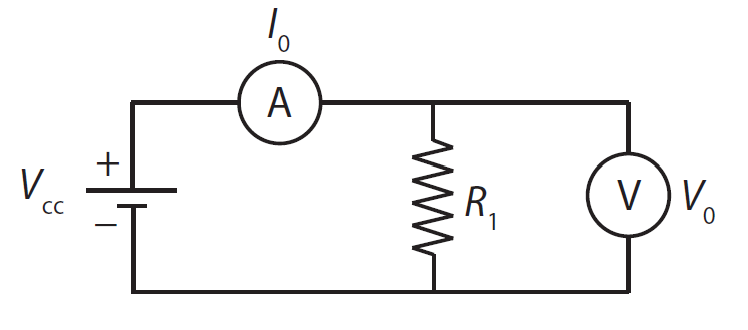
\includegraphics[width=0.5\textwidth]{img/parte (a).png}
\end{figure}

%% FIGURA item b) [simplificado y sin medidores]
\begin{figure}[H]
\caption{Circuito eléctrico equivalente al de la primera actividad con los medidores removidos formado en LTspice}
\centering
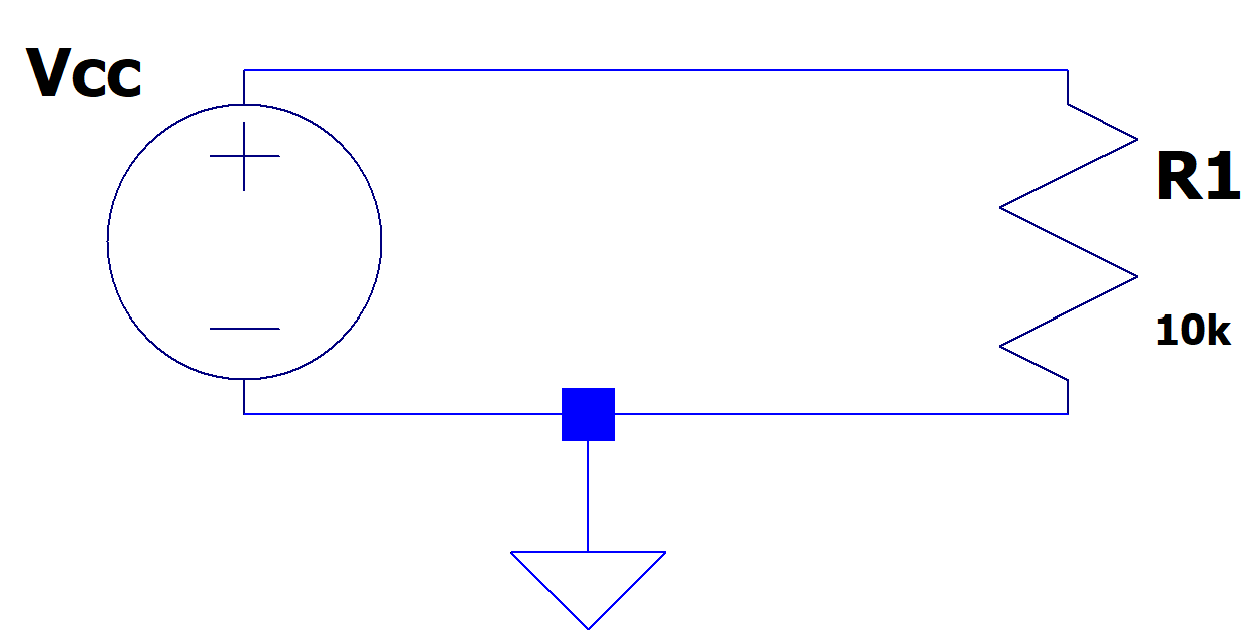
\includegraphics[width=0.4\textwidth]{img/parte c y d/circuito_1.png}
\end{figure}
\\ \\
%%%%% ITEM b)
Luego se procede a medir la corriente y voltaje en el circuito, con cinco valores distintos para la fuente de poder. Estos valores son 4, 6, 8, 10 y 12V. Todo esto se registra en una tabla (tabla 2) que incluye el cociente del voltaje con la corriente, correspondiente a la resistencia medida.
\\  \\


%%%%%% ITEM c) 
Como tercera parte se repite lo anterior, se arma el circuito de la figura 1 en LTspice, pero esta vez incluyendo los medidores como se indica en la figura 3. Para el amperímetro se escoge como resistencia interna el valor de 1$[\Omega]$ en el programa, este debe ser de un valor pequeño para no disminuir la corriente ni interferir en el circuito cuando se mida. Por otro lado para implementar el voltímetro, se le asigna un valor de $1Mega [\Omega]$ como resistencia interna, el valor debe ser alto para que no interfiera con la corriente que pasa por la resistencia medida. Nuevamente los valores obtenidos se registran en una tabla. (Tabla 3)

\\ \\

\begin{figure}[h]
\caption{Circuito equivalente al de la primera actividad, incluidos los medidores, formado en LTspice.}
\centering
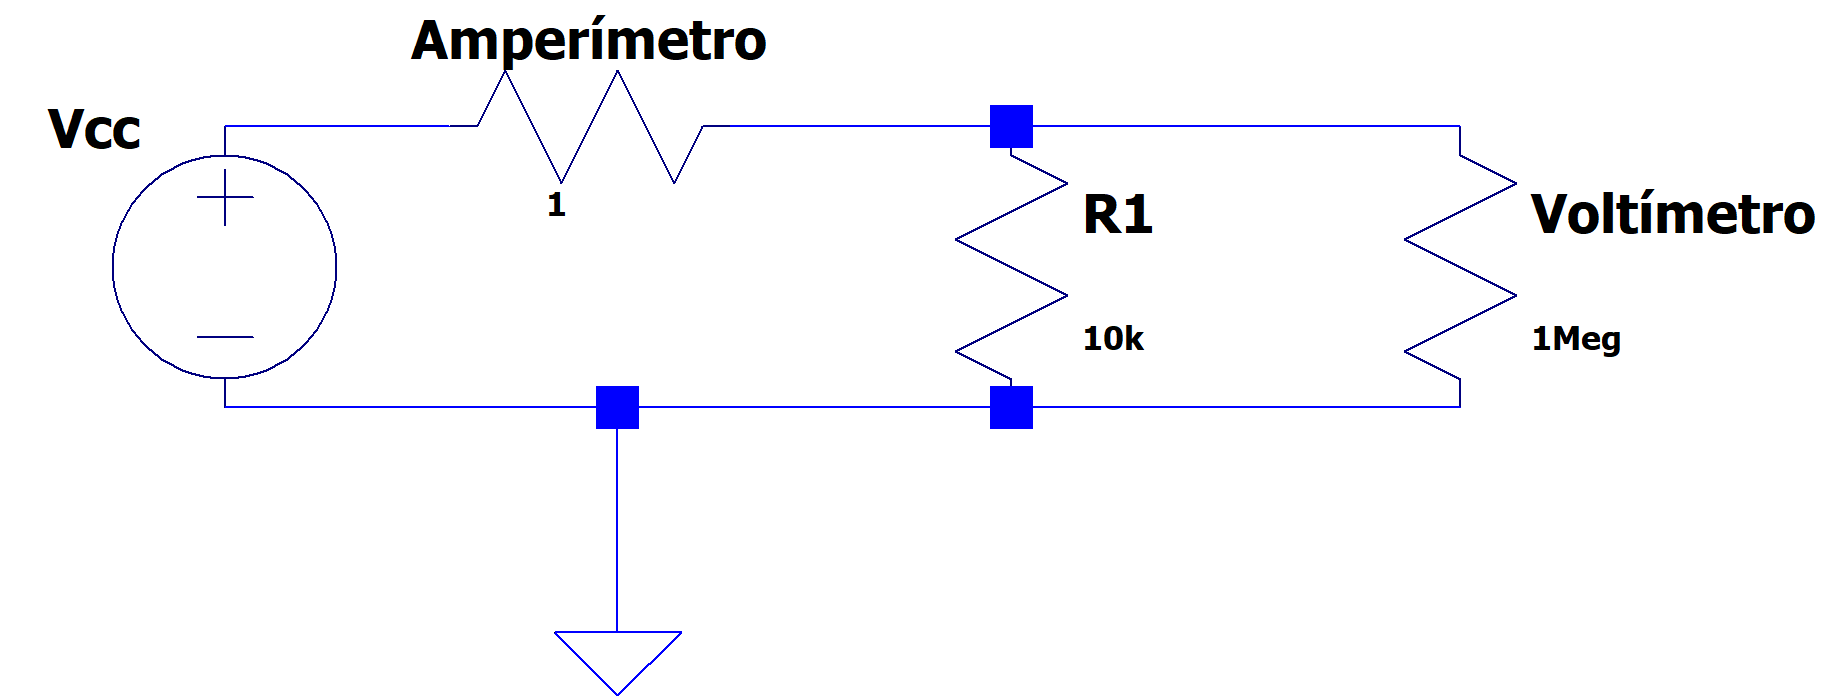
\includegraphics[width=0.6\textwidth]{img/parte c y d/circuito_2.png}
\end{figure}
%%%%%%%%%%%
%Parte e (y d implícitamente)
%%%%%%%%%%%%%%%%%
Con los datos recolectados en la tercera parte de la experiencia (correspondientes a la tabla 2) se calcula el promedio y desviación estándar del cociente entre voltaje $V_0$ y corriente $I_0$ medidos sobre la resistencia y se presentan en su respectiva tabla. (Tabla 4) 
%%%%%%%%%%%%%%%%%%%%%
%Parte f
Así se procede a realizar dos gráficos de $V_0$
en función de la corriente $I_0$, usando los datos de la segunda y tercera parte. Se realiza un ajuste lineal en cada gráfico para verificar que ambos casos cumplan con la ley de Ohm. Se recomienda usar la función polyfit en caso de usar Matlab, Octave o la librería $matplotlib$ de Python en los gráficos.
%%%%%%%%%%%%%%%%%%%%%%p
%parte g a la basura xdxd
%%%%%%%%%%%%%%%%%%%%%%%%55
\\ \\
Finalmente, se vuelve al circuito eléctrico con medidores de la figura 2. Se conserva la resistencia interna del amperímetro en 1$[\Omega]$, y se cambian los valores de la resistencia interna del voltímetro con el fin de encontrar cuando pierde valor su medición.

Los valores otorgados a la resistencia interna del voltímetro son: 1000K, 800k,700k, 200k, 100k , 90k y 80k $[\Omega]$.

La pérdida de validez del voltímetro se ve a partir del valor de la resistencia equivalente. Al considerar el voltímetro como una resistencia más se tiene que en el circuito de la figura 3, se comporta como un circuito paralelo, sin considerar el amperímetro:
$$
 \frac{1}{R_{eq}}=\frac{1}{R_{nominal}}+\frac{1}{R_v}=\frac{1}{10k}+\frac{1}{R_{v}} & \Rightarrow R_{eq}=10k\left (\frac{R_v}{R_v+10k}  \right )
$$
Donde $R_v $ es la resistencia interna del voltímetro y $R_{eq}$ es la resistencia equivalente. 

El voltímetro deja tener validez cuando la resistencia equivalente difiere de la resistencia nominal en más de un 10\%, equivalentemente, $\left (\frac{R_v}{R_v+10k}  \right )<0.9$, equivalente a $\Delta\% R= \left (1-\left (\frac{R_v}{R_v+10k}  \right )\right )*100\%<10\% $.




\subsection{Segunda experiencia: Leyes de Kirchhoff}
La segunda experiencia parte con escoger tres resistencias de medidas 1k, 5k y 10k $[\Omega]$, respectivamente. Se calcula la resistencia equivalente en serie y en paralelo. Para luego conectar las resistencias en serie y en paralelo en un circuito de LTspice, con una fuente de poder de 12 V, como se observan en las figuras 4 y 5, respectivamente.

Luego se procede a medir la corriente y el voltaje 
en cada circuito con las herramientas de LTspice,
para calcular la resistencia medida utilizando la ley
Ohm. Las resistencias medidas y calculadas se registran
en una tabla.

Se utilizan en este caso las herramientas de medir de LTspice
y no un amperímetro y voltímetro, para medir directamente
la corriente y voltaje, con el fin de que sean lo más precisos posibles.
\begin{figure}[H]
\caption{Circuito eléctrico en serie formado en LTspice, $V_1$ representa el voltaje, y $R_1,R_2$ y $R_3$ corresponden a las resistencias.}
\centering
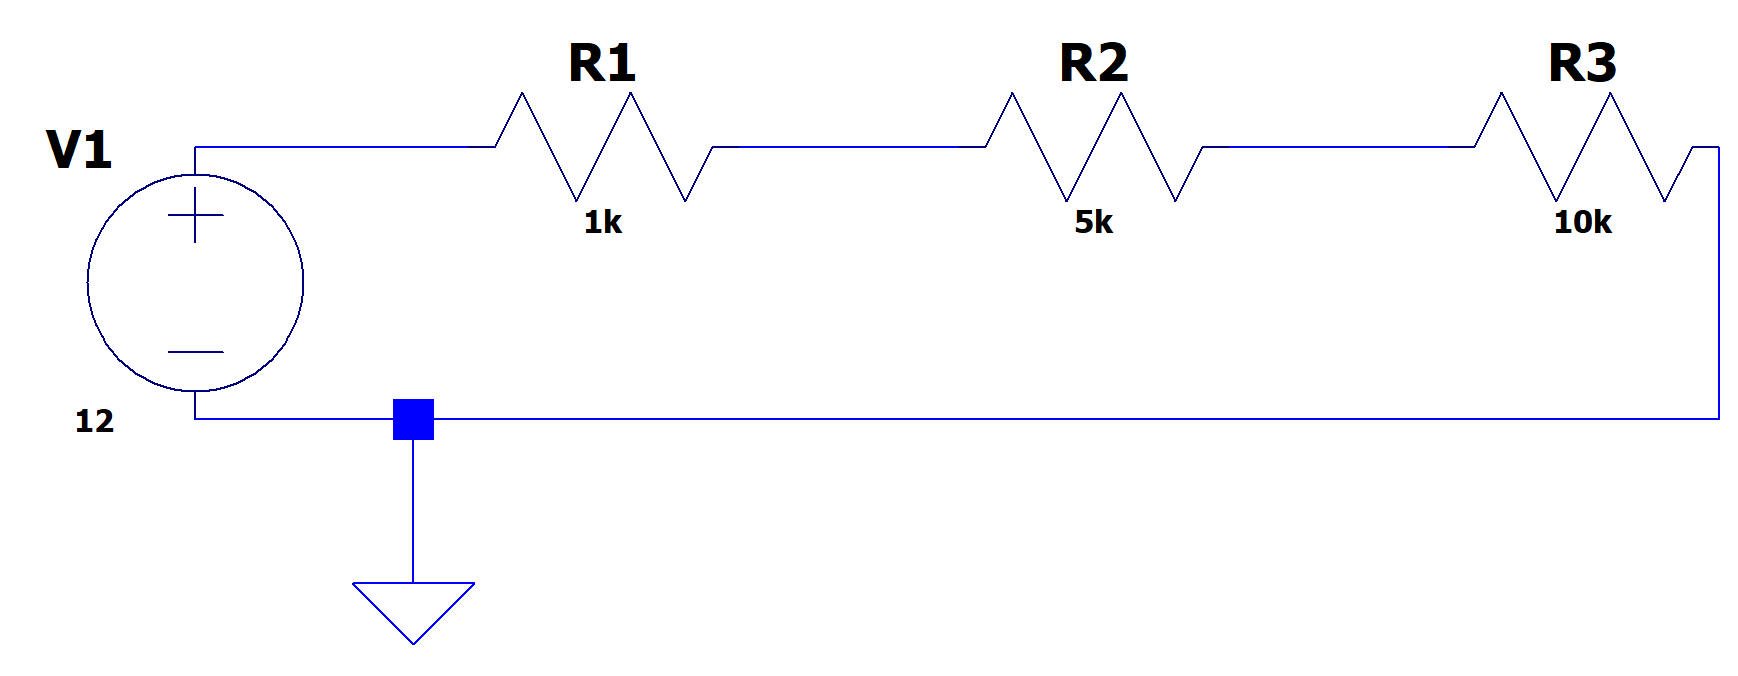
\includegraphics[width=0.5\textwidth]{img/parte i y j/circuto en serie.png}
\end{figure}
%%%%%%%%%%%%%%%%%%%%
%Parte j
%% FIGURA item b) [simplificado y sin medidores]
\begin{figure}[H]
\caption{Circuito eléctrico en paralelo formado en LTspice, $V_1$ representa el voltaje, y $R_1,R_2$ y $R_3$ corresponden a las resistencias.}
\centering
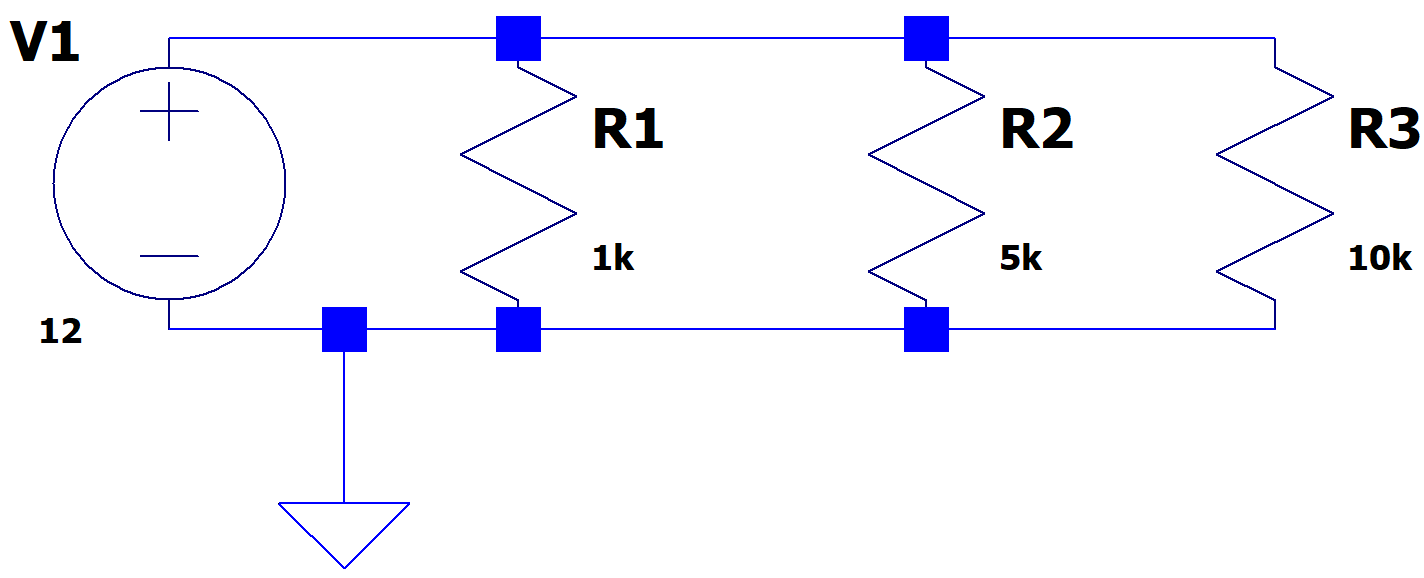
\includegraphics[width=0.45\textwidth]{img/parte i y j/circuito en paralelo.png}
\end{figure}
En la segunda parte se vuelve al circuito de resistencias en serie, como se muestra en la figura 4, y se procede a medir la corriente $I_0$ en el circuito, y el voltaje $V_{R1},V_{R2} $ y $V_{R3}$ sobre las resistencias $R_1, R_2$ y $R_3$ respectivamente. Para medir la corriente se usa un amperímetro con una resistencia interna de 1$[\Omega]$, que se conecta en serie como se indica en la primera imagen de la figura 6. Y para cada resistencia se coloca un voltímetro, de resistencia interna $1 Mega [\Omega]$, que se conecta en paralelo para medir el voltaje como se indican en el segundo, tercer y cuarto paso de la figura 6. La fuente de poder es de 12 V.


\begin{figure}[H]
\caption{Circuito eléctrico de resistencias en serie formado en LTspice, con sus medidores amperímetro y voltímetro.}
\centering
\includegraphics[width=0.45\textwidth]{img/parte k/4.png}
\includegraphics[width=0.45\textwidth]{img/parte k/1.png}
\includegraphics[width=0.45\textwidth]{img/parte k/2.png}
\includegraphics[width=0.45\textwidth]{img/parte k/3.png}
\end{figure}
En la tercera parte se vuelve al circuito de resistencias en paralelo como se muestra en la figura 5, y se procede a medir el voltaje $V_0$ sobre el circuito, y las corrientes $I_{R1},I_{R2}$ e $I_{R3}$ sobre las resistencias $R_1, R_2$ y $R_3$ respectivamente.
Para medir el voltaje su usa un voltímetro, de resistencia interna de $1 Mega [\Omega]$, que se conecta en paralelo como aparece en la primera imagen de la figura 7. Para medir la corriente en cada resistencia se usa un amperímetro, de resistencia $1[\Omega]$, que se conecta en serie  como aparecen en la segunda, tercera y cuarta imagen de la figura 7. La fuente de poder es de $12 V$. 

\begin{figure}[H]
\caption{Circuito eléctrico de resistencias en serie formado en LTspice, con sus medidores  amperímetro y voltímetro.}
\centering
\includegraphics[width=0.25\textwidth]{img/parte final/voltímetro.png}
\includegraphics[width=0.20\textwidth]{img/parte final/ampI1.png}
\includegraphics[width=0.20\textwidth]{img/parte final/ampI2.png}
\includegraphics[width=0.20\textwidth]{img/parte final/ampI3.png}
\end{figure}
\newpage 
\section{Resultados}
\subsection{Primera experiencia: Ley de Ohm}
A continuación, se presenta el calculo para la resistencia medida en la primera parte,
$$ R_{medida}=\frac{V}{I}=\frac{10,32 \pm 0,005}{1,01\pm0,005}\left [ 
\frac{V}{mA}\right ]=10.217,51\pm 50,88 [\Omega] \approx 10.218\pm51[\Omega] $$
La tabla 1 muestra el valor de la resistencia nominal junto a la resistencia medida y su error de medición.
\begin{center}
\begin{tabular}{|c|c|c|}
\hline
$R_{nominal} [$\Omega$]$ & $R_{medida}[$\Omega$]$    & $\Delta R_{medida}[$\Omega$]$ \\ \hline
10k     & 10.218  & 51          \\ \hline
\end{tabular}
\end{center}{}
La tabla 2 muestra los resultados de medir el circuito que no posee instrumentos de medición. (Figura 2)
\begin{center}

 \vspace*{1mm} \\
\begin{tabular}{|c|c|c|}
\hline
$V_0[V]$ & $I_0[mA]$ & $\frac{V_0}{I_0}[k\Omega]$ \\ \hline
4     & 0,4 & 10             \\ \hline
6     & 0,6 & 10            \\ \hline
8     & 0,8 & 10            \\ \hline
10    & 1   & 10             \\ \hline
12    & 1,2  & 10            \\ \hline
\end{tabular}
\end{center}
La tabla 3 muestra los resultados de medir el circuito que incluye los instrumentos de medición. (Figura 3)
\begin{center}
 \vspace*{1mm} \\
\begin{tabular}{|c|c|c|}
\hline
$V_0[V]$ & $I_0[mA]$ & $\frac{V_0}{I_0}[k\Omega]$ \\ \hline
4.000   & 0.404  &       9,900             \\ \hline
5.999   & 0.606   &      9,899             \\ \hline
7.999   & 0.808   &      9,900             \\ \hline
9.999   & 1.01    &      9,900             \\ \hline
11.999  & 1.212  &       9,900                  \\ \hline
\end{tabular}
\end{center}
La tabla 4 muestra el promedio y la desviación estándar del cociente entre voltaje $V_0$ y corriente $I_0$ sobre la resistencia usada en la tabla 2. (Figura 2)
\begin{center}
\vspace*{1mm} \\
\begin{tabular}{|c|c|}
\hline
$\langle \frac{V_0}{I_0}\rangle$ & $\sigma$ \\ \hline
10                               & 0        \\ \hline
\end{tabular}
\end{center}
%%%%%%%%%%%%%%%%%%%%%%%%%%%
%GRAFICOS%%%%%%%%%%%%%%%%%%%%

% parte (f)
La figura 8 presenta la proporcionalidad entre voltaje e intensidad de corriente que se observan en el circuito sin medidores
\begin{figure}
    \centering
    \includegraphics[width=0.75\textwidth]{img/graficos f/act_f figura sin medidores.png}
    
    \caption{Intensidad en función del Voltaje para el circuito sin medidores.}
    \label{fig:my_label}
\end{figure}

A continuación, la figura 9 presenta la proporcionalidad para el mismo circuito pero incluyendo los instrumentos medidores:
\begin{figure}
    \centering
    \includegraphics[width=0.75\textwidth]{img/graficos f/act_f figura con medidores.png}
    
    \caption{Intensidad en función del Voltaje para el circuito con medidores.}
    \label{fig:my_label}
\end{figure}


%%%%%%%%%%%%%%%%%%%%%%%%%
%%%%%%%%%%%%%%%%%%%%%%%%%
La tabla 7 muestra los valores que toma la resistencia interna del voltímetro y el error porcentual entre la resistencia equivalente y la nominal que conlleva.
\begin{center}
\begin{tabular}{|c|c|}
\hline
$R_v [\Omega]$ & $\Delta \% R$ \\ \hline
1000k          & 0.99\%       \\ \hline
800k           & 1.23\%       \\ \hline
200k           & 4.74\%       \\ \hline
100k           & 9.09\%       \\ \hline
90k            & 10\%         \\ \hline
80k            & 11.11\%      \\ \hline
\end{tabular}
\end{center}{}

\subsection{Segunda experiencia: Leyes de Kirchhoff}
A continuación se presentan el desarrollo para las resistencias para los circuitos en serie y en paralelo, de la figura 4 y 5 respectivamente.

Sean $R_1=1k[\Omega]$,$R_2=5k[\Omega]$ y $R_3=10k[\Omega]$.
\begin{enumerate}
    \item Resistencias en serie:
    $$ R_{calculada}=R_1+R_2+R_3=1k+5k+10k [\Omega]=16k [\Omega]$$
    \item Resistencias en paralelo:
    $$\frac{1}{R_{calculada}}=\frac{1}{R_1}+\frac{1}{R_2}+\frac{1}{R_3}=\frac{1}{1k}+\frac{1}{5k}+\frac{1}{10k} ~~\left [ \frac{1}{\Omega}   \right ]$$
    $$ \frac{1}{R_{calculada}}=\frac{13}{10k}\left [ \frac{1}{\Omega}   \right ]\implies R_{calculada}=\frac{10}{13}k [\Omega]$$
La tabla 8 muestra la comparación entre las resistencias calculadas y medidas de los circuitos de las figuras 4 y 5.
\end{enumerate}{}
\begin{center} \vspace*{1mm} \\
\begin{tabular}{|c|c|c|}
\hline
            & $R_{paralelo} [\Omega]$ & $R_{serie} [\Omega]$ \\ \hline
Calculada   &     $\frac{10}{13} k$     &   $16K$            \\ \hline
Medida      &     $\frac{10}{13} k$     &   $16K$            \\ \hline
\end{tabular}\\
\end{center}
En la tabla 9 se muestran los resultados de las mediciones de voltaje en cada una de las resistencias y corriente del circuito en serie. (Figura 6) 
% parte k)
\begin{center}
    Comparación para valores medidos con Voltaje $V_{cc}$ de Resistencias en serie
    \begin{tabular}{|c|c|c|c|c|}
    \hline
         $V_{cc} [V]$ & $V_{R1} [V]$ & $V_{R2} [V]$ & $V_{R3} [V]$ & $I_{0} [mA]$  \\ \hline
            $12$  & $0.7493$ & $3.7371$ &  $7.4720$ & $0.749$ \\ \hline 
    \end{tabular}
\end{center}
Por la ley de voltajes, se tiene que
$$V_{cc}=V_{R1}+V_{R2}+V_{R3}=0.7493+3.7371+7.4720 [V]= 11.958 [V]$$
En la tabla 10 se muestran los resultados de las mediciones de corriente en cada una de las resistencias y voltaje del circuito en serie. (Figura 7) 
% parte m)
\begin{center}
    Comparación para valores medidos con Voltaje $V_{cc}$ de Resistencias en paralelo
    \begin{tabular}{|c|c|c|c|c|}
    \hline
        $V_{cc} [V]$ & $I_{R1} [A]$ & $I_{R2} [A]$ & $I_{R3} [A]$ & $V_{0} [V]$ \\ \hline
        $12$ & $0.012$ & $0.002$ & $0.001$ & $$12$$ \\ \hline
        
    \end{tabular}
\end{center}
De la primera parte, la resistencia equivalente del circuito en paralelo es, $R_{eq}=\frac{10}{13}k[\Omega]$.

Usando este valor para la resistencia equivalente y la ley de Ohm, se puede determinar que la intensidad de corriente del circuito equivale a:
$$I_0=\frac{V_0}{I_0}=\frac{12 [V]}{\frac{10}{13}k[\Omega]}=0.0156 [A] $$
Y para verificar la ley de corrientes basta con ver que la suma de las intensidades de corriente medidas experimentalmente en los nodos de las resistencias es idéntico al valor teórico: 
$$I_0^{*}=I_{R1}+I_{R2}+I_{R3}=0.012+0.002+0.001~~ [A]= 0.0155[A]$$
En consecuencia, si se suman las medidas de corrientes que entran al sistema y se restan las que salen por los nodos se tiene que:
$$\sum_{sistema}{I}:=I_0 - I_1 - I_2 - I_3 = (0.0156 - 0.012 - 0.002 - 0.001) [A] = (0.0156 - 0.0155) [A] = 0.0001 [A]$$
Verificando efectivamente que se cumple la ley de corrientes de Kirchhoff.




\newpage
\section{Análisis}
%
\subsection{Primera experiencia: Ley de Ohm}
Los resultados obtenidos de la medición realizada en el circuito construido en la actividad b) de la primera experiencia muestran un claro comportamiento lineal, donde el crecimiento de la intensidad de corriente es directamente proporcional al voltaje utilizado en la fuente de poder. \\

Así mismo los resultados obtenidos de la medición realizada del circuito montado como sugiere la actividad d), esta vez con la inclusión de medidores, muestra una clara tendencia lineal a pesar de las interferencias incidentes en el circuito debido a los instrumentos de medición. Se sigue conservando la constante de proporcionalidad con diferencias de orden mínimo por la interferencia de los instrumentos especificada anteriormente. \\

En la actividad siguiente se calcula el promedio y desviación estándar del cociente entre el voltaje ($V_0$) y la intensidad de corriente ($I_0$), se obtiene $10 [k\Omega]$ como promedio y una desviación nula, lo cual es razonable y esperable ya que el cociente se mantiene constante en las mediciones debido a la proporcionalidad directa y el cociente es, de hecho, la constante de proporcionalidad. \\

Posteriormente, en el primer gráfico elaborado para la actividad f) se puede apreciar el gráfico que ilustra el comportamiento del circuito ensamblado en la actividad b) correspondiente al primer circuito, pero simplificado removiendo sus medidores. Es directo notar que la tendencia de los valores sigue la tendencia lineal que se mencionó anteriormente.\\

Continuando con la actividad f), también se confeccionó un gráfico que representa visualmente el comportamiento del circuito armado en la actividad d) que corresponde al primer circuito con los medidores incluidos, el gráfico es idéntico al anterior puesto que los valores obtenidos en esta actividad diferían de los primeros en valores del orden de $10^{-3}$ por lo que la estructura del comportamiento lineal se sigue manteniendo. \\

Al final de la primera experiencia se adjunta una tabla en los resultados que contiene información sobre distintas mediciones hechas para valores diferentes en la resistencia interna de un voltímetro y sus respectivos errores con el fin de afirmar cuando un voltímetro se podría considerar válido, de esta manera se puede ver que el error de medición disminuye a medida que aumenta el valor de la resistencia de manera no lineal. 

\subsection{Segunda experiencia: Leyes de Kirchhoff}
El primer resultado adjunto en la segunda experiencia corresponde al desarrollo para el cálculo del valor de la resistencia teórica de un circuito conformado por tres resistencias conectadas en paralelo y en serie. \\ A continuación del primer resultado se presenta una tabla donde se comparan los valores teóricos obtenidos a través de la Ley de Ohm con los valores medidos experimentalmente recreando los circuitos LTspice. Los resultados son exactamente equivalentes. \\

En el siguiente resultado se tiene una tabla donde se presentan los resultados obtenidos al medir los voltajes de cada una de las resistencias dado un voltaje $V_{cc}$ fijo para el circuito con las resistencias conectadas en serie. Se puede apreciar en el cálculo que se muestra a continuación que el valor dado por la suma es muy cercano al valor del voltaje del circuito verificando efectivamente la ley de voltajes de Kirchhoff. % En discusión se debe comentar sobre esto, por qué ocurre? Se debe a que las resistencias interfieren? Errores sistemáticos? etc

Finalmente, el último resultado de la segunda experiencia presenta una tabla donde se exponen los resultados obtenidos al medir las intensidades que entran a cada una de las resistencias dado también un voltaje $V_{cc}$ fijo para el circuito con las resistencias dispuestas en paralelo. Se muestra en el cálculo adjunto posteriormente que la suma de la intensidad de corriente que entra al sistema y la resta de las que salen por los nodos es un valor idéntico a $0$. % Por qué no es exactamente 0? (ver en DISCUSIÓN)



\newpage
\section{Discusión}
\subsection{Primera experiencia: Ley de Ohm}
En la primera parte de la experiencia se comprueba que el valor de la resistencia del circuito de la figura 1 sea de $R_{nominal}=10k [\Omega]$. Esto se hace a partir de las medidas tomadas de la corriente y voltaje que se entregan, esto junto a la ley de Ohm y utilizando propagación de errores, entrega que $R=10.218\pm 51[\Omega]$. El resultado difiere en aproximadamente un 2\% del valor esperado, así se considera que el valor obtenido es plausiblemente aceptable.\\

Luego en la segunda parte se trabajó con el mismo circuito en el programa en LTspice. Variando el voltaje de la fuente de poder, se mide la corriente. Para así calcular el cociente del voltaje con la corriente medidos con el programa, lo cual según la ley de Ohm es el valor de la resistencia del circuito, o sea, $10k[\Omega]$. Lo cual lo hace con una gran exactitud, ya que entrega en cada caso el valor esperado.\\

En la tercera parte, se repite el proceso anterior solo que ahora se le agrega un amperímetro y voltímetro al circuito en LTspice. Como resultado entrega valores un poco más diferidos, respecto la resistencia medida, $\frac{I_0}{V_0}$, la diferencia es solo del orden de las milésimas. Lo cual termina siendo en una diferencia porcentual respecto a la resistencia nominal de aproximadamente un 1\%.\\

Volviendo a la primera parte se calcula el promedio del cociente entre el voltaje y corriente medidos, es decir, resistencia medida según ley de Ohm. El valor de este promedio es exactamente 10k$[\Omega]$, y la desviación estándar es nula. Así se tiene que la ley de Ohm se cumple en este circuito a los distintos tipos de voltaje aplicados.\\

Con los datos medidos del circuito con y sin medidores en la parte anterior, se realiza un gráfico, para cada uno, de $V_0$ en función de la corriente $I_0$. En ambos casos se realiza un ajuste lineal que corresponde a la tendencia que debería seguir si es que cumple con la ley de Ohm. De esto cabe notar que todos los puntos están por sobre la línea tal como se muestra en ambos gráficos. Por lo que en ambos se puede decir que cumplen con la ley.\\

Si es que en las actividades anteriores se reemplazara la resistencia por una ampolleta, la ley de Ohm no se cumpliría ya que una ampolleta necesita más voltaje para pasar corriente entre sus extremos debido a que esta disipa energía. Así, esta no cumple con el comportamiento lineal que se espera de la Ley de Ohm como se puede notar en los gráficos anteriores. Por su composición se dice que tienen un comportamiento cuadrático.\\

Finalmente usando el circuito con los medidores se procede a variar los valores de la resistencia interna del voltímetro con el fin de encontrar una configuración donde el instrumento pierda validez para medir, el amperímetro mantiene su valor respecto a la resistencia interna. En la tabla 7 se observan los diferentes valores que toma la resistencia del voltímetro y el error porcentual que esta conlleva en la resistencia equivalente del sistema respecto a la resistencia nominal. Explicando esto un poco más, al disminuir el valor de la resistencia del voltímetro este colabora en que la resistencia equivalente del circuito aumente con respecto de lo que era al principio (sin medidor), es decir, $10k[\Omega]$. Así, cuando la resistencia es de $90k[\Omega]$ o menos, el error es de mas de un 10\% por lo que se puede decir el instrumento dejaría de ser válido para medir. \\

La importancia de que la resistencia interna sea alta es que el voltímetro no interfiera con la corriente con los valores que registre el amperímetro. Así los valores de corriente que pasen por él deben ser idealmente menores que los valores que pueda registrar el amperímetro.




\subsection{Segunda experiencia: Leyes de Kirchhoff}

Al comienzo de la segunda experiencia se tiene que la resistencia medida es exactamente igual que la resistencia calculada por lo que se vuelve importante notar que debido a que el contexto de estas mediciones se hace en un entorno simulado por software, la probabilidad de que se presenten errores aleatorios en la medición es nula o prácticamente cero. \\ 

Posterior a la primera actividad de la segunda experiencia para verificar la Ley de Voltajes de Kirchhoff se verifica si la suma de los voltajes de cada una de las componentes del circuito es igual al voltaje completo del circuito y se obtienen valores idénticos, sin embargo, no son exactamente iguales. Además para la última actividad de la segunda experiencia se hace un razonamiento análogo para verificar la Ley de Corrientes de Kirchhoff donde se verifica si la intensidad de corriente que ingresa al circuito es igual a la que sale por los nodos donde se obtiene que de la resta para comparar estos valores se consigue un valor muy cercano a $0$ pero que sin embargo es distinto. La razón de este fenómeno se debe a la interferencia que causan los valores de las resistencias internas de los instrumentos de medición en el funcionamiento del circuito, alterando levemente los valores de la medición experimental. Es importante tener esto en cuenta ya que fuera de un entorno simulado estas diferencias en las medidas se pueden presentar en conjunto con otros posibles errores aleatorios, sin embargo, considerando que las Leyes consideran instrumentos de medición ideales es razonable la diferencia que se tiene entre los valores obtenidos pues son de orden muy pequeño y por lo tanto fáciles de detectar y controlar.

\newpage
\section{Conclusiones}

A través de las actividades realizadas en ambas experiencias se introdujeron conceptos básicos e intuición en relación al funcionamiento de circuitos eléctricos sencillos, también se pudo comprobar experimentalmente tanto la ley de Ohm como las leyes de Kirchhoff y por otro lado, la realización de las experiencias permitió ilustrar acerca del procedimiento para la utilización de instrumentos de medición como el Voltímetro y Amperímetro.

Es de alta importancia notar que algunos de los resultados obtenidos durante las experiencias son poco realistas y muy optimistas (por ejemplo, en la actividad d) $\sigma = 0$) ya que al encontrarse en un ambiente simulado se descartan los posibles errores aleatorios de factores no controlables del entorno del experimento y por lo tanto no aparece dispersión en los datos de las muestras.

Acerca de la herramienta utilizada para la experiencia (LTspice), si bien en su funcionamiento no deja de ser práctico y cumplir con su objetivo, su interfaz es un poco anticuada en estándares actuales del diseño de software por lo que al comienzo puede resultar poco intuitivo y algo abrumador para el usuario.


% Y vivieron felices para siempre
%             FIN 
% XD
% ayuda esto no es un meme :c 
\end{document}